\documentclass[12pt, a4paper]{report}

\usepackage[utf8]{inputenc}
\usepackage{geometry}
 \geometry{
 a4paper,
 total={170mm,257mm},
 left=20mm,
 top=20mm,
}

\usepackage{titlesec}
\titleformat
{\chapter}
[display]{\bfseries\Large\itshape}
{Capitolo Nr.\thechapter}
{0.5ex}
{
    \rule{\textwidth}{1pt}
    \vspace{1ex}
	\centering
}
[\vspace{-0.5ex}\rule{\textwidth}{0.3pt}]

\renewcommand{\contentsname}{Indice}

\usepackage{amsthm}
\usepackage{amsmath}
\usepackage{amsfonts}
\usepackage{amssymb}
\usepackage{enumitem}
\usepackage{latexsym}
\usepackage{systeme}
\usepackage{mathtools}
\usepackage{wasysym}
\usepackage{eurosym}
\usepackage{dsfont}
\usepackage{csquotes}
\usepackage{pgfplots}
\pgfplotsset{compat=1.15}

\theoremstyle{definition}
\newtheorem{definition}{Definizione}[section]
\newtheorem{theorem}{Teorema}[section]
\newtheorem{corollary}{Corollario}[theorem]
\newtheorem{lemma}[theorem]{Lemma}
\newtheorem*{demonstration}{Dim}
\newtheorem*{proposition}{Prop}
\newtheorem*{observation}{Oss}
\newtheorem*{property}{Proprietà}
\newtheorem*{note}{NB}

% Crea un nuovo comando
\DeclareRobustCommand{\F}{\mathcal{F}}%Fa il simbolo di tribù
\DeclareRobustCommand{\R}{\mathbb{R}}% simbolo dell'insieme dei numeri reali
\DeclareRobustCommand{\N}{\mathbb{N}}%simbolo dei naturali
\DeclareRobustCommand{\B}{\mathcal{B}}% simbolo dei Boreliani
\DeclareRobustCommand{\supp}{\mathcal{R}}%simbolo del supporto
\DeclareRobustCommand{\powerset}{\mathcal{P}(\Omega)}
\DeclareRobustCommand{\tribedef}{\F\subseteq \powerset}
\DeclareRobustCommand{\tribe}{\F=\powerset}
\DeclareRobustCommand{\probspace}{(\Omega,\F,P)}
\DeclareRobustCommand{\probzspace}{(\Omega,\F)}
\DeclareRobustCommand{\partitionInI}{\{E_i\}_{i\in I}}
\DeclareRobustCommand{\one}{\mathds{1}}
\DeclareRobustCommand{\norm}{\mathcal{N}}
\newcommand\underrel[2]{\mathrel{\mathop{#2}\limits_{#1}}}% Scritte sotto un simbolo
\newcommand\conv[2]{\xrightarrow[#2\to +\infty]{#1}}

\title{Dispense di Probabilità e Statistica}
\author{Leonardo De Faveri}
\date{}

\usepackage{xcolor}
\usepackage{hyperref}
\hypersetup{
  colorlinks,
  linkcolor={red!90!black},
  citecolor={blue!50!black},
  urlcolor={blue!80!black}
  pdftitle={Dispense di algoritmi e strutture dati},
  pdfpagemode=FullScreen,
}

\begin{document}
\maketitle
\tableofcontents

\chapter{Introduzione}

\section{Definizione di Probabilità}
La Probabilità permette di misurare l'incertezza; l'incertezza può essere dovuta
del tempo, da una misurazione, dallo spazio e dai casi e/o soggetti.

\section{Statistica descrittiva e inferenziale}
La \emph{Statistica descrittiva} studia tutta la popolazione, mentre la 
\emph{Statistica inferenziale} ne studia solo un campione e successivamente usa 
quel risultato per stimare la quantità interessata nell'intera popolazione.

\section{Cenni di teoria degli insiemi}
Un insieme è definito come una collezione di oggetti detti elementi.\newline
La nozione di appartenenza può essere messa a fondamento di tutta la teoria
degli insiemi:
\begin{definition}
	Scriveremo \(x\in A\) intendendo che $x$ è un elemento dell'insieme $A$,
	mentre diremo che \(y\notin A\) intendendo che $y$ non è un elemento di $A$.
\end{definition}
\begin{property}
	Dato un insieme $A$, $\forall x$ si deve essere in grado di stabilire
	se $x$ appartiene o meno all'insieme $A$.
\end{property}

\noindent
Valgono i seguenti assiomi:
\begin{enumerate}[label=(\roman*)]
	\item \emph{Estensionalità}: Dati 2 insiemi $A, B$, vale \(A=B
	\Leftrightarrow \forall x: x \in A \Leftrightarrow x \in B\)
	\item \emph{Insieme vuoto}: Il simbolo $\emptyset$ identifica un insieme
	privo di elementi
	\item \emph{Separazione}: Sia $X$ un insieme. Supponiamo che a ogni elemento 
	$x\in X$ sia associata un'affermazione $P(x)$ dipendente da $x$. Allora:
	\[ \{x | x\in X,\ P(x)\ \text{è vera} \} = \{x\in X | P(x)\} \]
	è un insieme.
\end{enumerate}

\begin{definition}
	Siano $X$ e $Y$ due insiemi. Scriveremo $X\subset Y$ se è vero che 
	$\forall x\in X \Rightarrow x\in Y$, ma non il contrario. E diremo che $X$
	è un \emph{sottoinsieme proprio} di $Y$.
\end{definition}
\begin{definition}
	Siano $X$ e $Y$ due insiemi. Se $X\subset Y$ e $X=Y$ allora $X$ viene detto
	\emph{sottoinsieme} di $Y$ e in simboli si scrive $x\subseteq Y$.
\end{definition}

\subsection{Operazioni sugli insiemi}
Siano $X$ e $Y$ due insiemi, definiamo:
\begin{itemize}
	\item \emph{Unione}: \(X\cup Y = \{x | x\in X\ \text{o}\ x\in Y\}\)
	\item \emph{Intersezione}: \(X\cap Y = \{x | x\in X,\ x\in Y\}\)
	\item \emph{Differenza}: \(X \symbol{92} Y = \{x | x\in X, x\notin Y\}\)
	\item \emph{Differenza simmetrica}: \(X\bigtriangleup Y = (X \symbol{92} Y) \cup (Y \symbol{92} X) \)
	\item \emph{Prodotto cartesiano}: \(X\times Y = \{(x, y) | x\in X,\ y\in Y\}\)
\end{itemize}

\noindent
Se \(Y\subset X\) definiamo l'insieme complementare come segue:
\[C_X(Y) = Y^c = \{x | x\in X,\ x\notin Y\} = X \symbol{92} Y\]
\begin{note}
	La notazione $Y^c$ non specifica rispetto a quale insieme si sta calcolando 
	il complementare.
\end{note}

\noindent
Sia $I$ un insieme non vuoto. \(\forall i\in I \) sia $A_i$ un insieme.
Indichiamo il dato $I$ ($A_i$ con $i\in I$) scrivendo \(\{A_i\}_{i\in I} \).
Su questa famiglia d'insiemi definiamo:
\begin{itemize}
	\item \emph{Unione arbitraria}: \(\bigcup_{i\in I}A_i=\{x|\exists i\in I,\ x\in A_i\}\)
	\item \emph{Intersezione arbitraria}: \(\bigcap_{i\in I}A_i=\{x|\forall i\in I,\ x\in A_i\}\)
\end{itemize}

\noindent
\begin{definition}
	Dato un insieme $A$ e sua una famiglia di sottoinsiemi $S$.
	$S$ è detto \emph{partizione} se \(\forall x\in A\ \exists!B\in S | x\in B\).
\end{definition}
\begin{property}
	Dato un insieme $A$ e una sua partizione $S$ valgono le seguenti:
	\begin{enumerate}[label=(\roman*)]
		\item \(A = \bigcup_{B\in S}B\)
		\item \(\forall B, C\in S\text{ con }B\neq C\text{ vale }B\cap C=
		\emptyset\)
	\end{enumerate}
\end{property}

\subsection{Cardinalità di un insieme}
\begin{definition}
	Dato un insieme $A$ se ne definisce cardinalità il numero di elementi
	in esso contenuti e scriveremo in simboli $\#A$.
\end{definition}
\begin{property}
	Valgono le seguenti:
	\begin{enumerate}
		\item Siano $A$ un insieme e \(S=\{E_i\}_{i=1}^n\) una sua partizione.
		Allora \(\#A = \sum_{i=1}^{n}\#E_i\)
		\item Siano $A$ e $B$ due insiemi. \(\#(A\times B) = \#A \cdot  \#B\)
		\begin{note}
			\((A\times B)\neq (B\times A)\), ma \(\#(A\times B) = \#(B\times A)\)
		\end{note}
		\begin{observation}
			\(\# \otimes_{i=1}^n A_i=\prod_{i=1}^n A_i\)
		\end{observation}
		\item \(\#(A_1\cup A_2) = \#A_1 + \#A_2 - \#(A_1\cap A_2)\)
		\begin{observation}
			\(\#(A_1\cup A_2\cup A_3) = \#A_1 + \#A_2 + \#A_3 - \#(A_1\cap A_2)
			- \#(A_1\cap A_3) - \#(A_2\cap A_3) + \#(A_1\cap A_2\cap A_3)\)
			\\Vale un ragionamento analogo per famiglie più numerose di insiemi.
		\end{observation}
	\end{enumerate}
\end{property}

\chapter{Principi di calcolo combinatorio}

Nella probabilità classica la probabilità di evento è calcolata come il rapporto
tra il numero di casi favorevoli e il numero di casi totali:
\[ P(E) = \frac{\#F}{\#T} \]
Ma come si contano i casi favorevoli e totali? Usando il calcolo combinatorio.

\section{Permutazioni}
Le permutazioni permettono di rispondere alla domanda: \textit{In quanti modi
posso mettere in fila $n$ elementi di un insieme $A$?}
\\\textit{Risposta: $n!$}

\paragraph*{Esempio}
Quanti sono gli anagrammi della parola "Prendiamo"? 

Provo a procedere una lettera alla volta. La prima volta posso scegliere una tra
9 lettere, la seconda 8, le terza 7 e cosi via. Alla fine arrivo ad avere:
\(9\cdot 8\cdot 7\cdot 6\cdot 5\cdot 4\cdot 3\cdot 2\cdot 1 = 9!\)

\subsection{Permutazioni con ripetizioni}
\textit{Cosa succede se un elemento si ripete $m$ volte?}
\\\textit{Risposta: $\frac{n!}{m!}$}

\paragraph*{Esempio}
Quanti sono gli anagrammi della parola "Anagramma"?

Noto che le lettere \emph{a} ed \emph{m} si ripetono rispettivamente 4 e 2 volte.
Gli anagrammi possibili sono quindi:
\[\frac{n!}{a!\cdot  m!} = \frac{9!}{4!\cdot 2!} = \frac{9\cdot 8\cdot 7\cdot 6\cdot 5\cdot 4\cdot 3\cdot 2\cdot 1}{4\cdot 3\cdot 2\cdot 1\cdot 2\cdot 1}
= \frac{9\cdot 8\cdot 7\cdot 6\cdot 5}{2\cdot 1} = 9\cdot 8\cdot 7\cdot 5\cdot 3\]

\section{Disposizioni}
Le disposizioni rispondono alla domanda: \textit{In quanti modi posso mettere in
fila $m$ elementi tra gli $n$ di un insieme $A$}?
\\\textit{Risposta: \(\frac{n!}{(n-m)!}\)}

\paragraph*{Esempio}
Quante sono le parole di 4 lettere, tutte diverse, se l'alfabeto utilizzato
ha 26 lettere?

Provo a scegliere una lettera alla volta.
La Prima volta ho 26 possibilità, la seconda 25, le terza 24 e la quarta 23.
Posso quindi ottenere il risultato facendo: $26\cdot 25\cdot 24\cdot 23$.

\textit{E usando la formula?}
\\Devo innanzitutto scegliere i valori di $m$ e $n$. Siccome l'alfabeto ha 26
lettere pongo $n=26$ e, di conseguenza, $m=4$. Ora applico la formula:
\[\frac{n!}{(n-m)!} = \frac{26!}{(26 - 4)!} = \frac{26!}{22!} = 
\frac{26\cdot 25\cdot 24\cdot 23\cdot 22!}{22!} = 26\cdot 25\cdot 24\cdot 23\]

\subsection{Disposizioni con ripetizioni}
\textit{Cosa succede se alcuni elementi si ripetono?}
\\\textit{Risposta: $n^k$}

\paragraph*{Esempio}
Utilizzando le cifre $1,2,3$ quanti numeri di 4 cifre si possono formare?

Essendo le cifre tra cui scegliere meno rispetto a quelle da dover utilizzare ci
saranno sicuramente delle ripetizioni. In particolare, ogni cifra può ripetersi
fino a 4 volte. Se ora provo a immaginare di avere tanti cassetti quante sono le
cifre del numero da creare, quindi 4, e provo a creare il numero prendendo una
cifra alla volta, la prima volta potrò scegliere una cifra su 3. Siccome le cifre
si possono ripetere la seconda sarà ancora tra 3 cifre e così anche le altre.
Quindi avrò $3\cdot 3\cdot 3\cdot 3$ modi di formare un numero di 4 cifre.

\textit{E usando la formula?}
\\È sufficiente prendere $k=4$ e $n=3$ e applicare la formula:
\[n^k = 3^4\]
In particolare ho posto $k$ pari al numero di cassetti e $n$ pari al numero di
scelte che ho per ogni cassetto.

\section{Combinazioni}
Le combinazioni rispondono alla domanda: \textit{In quanti modi posso scegliere
$m$ elementi (in qualsiasi ordine) tra gli $n$ di un insieme $A$?}
\\\textit{Risposta: $\frac{n!}{(n-m)!\cdot m!} = \binom{n}{m} $}

\paragraph*{Esempio}
Quante sono le sestine formate da 6 numeri scelti tra 90?

Posso procedere in due passi
\begin{enumerate}
	\item Conto in quanti modi possono essere ordinati 6 numeri scelti tra 90
	\item Conto in quanti modi posso ordinare 6 numeri
\end{enumerate}
\noindent
Procedo:
\begin{enumerate}
	\item Il problema di contare i possibili ordinamenti di 6 numeri scelti tra
	90 è un tipico problema di \emph{disposizioni semplici}, quindi:
	\(n="\#sestine\ ordinate"=\frac{90!}{(90-6)!}\)
	\item I possibili ordinamenti di 6 numeri sono invece calcolabili sfruttando
	le \emph{permutazioni semplici}, quindi: \(m="\#numero\ ordinamenti"=6!\)
\end{enumerate}
\noindent
A questo punto mettendo insieme i risultati si ottiene:
\[\frac{n}{m} = \frac{90!}{(90-6)!}\cdot \frac{1}{6!} = \frac{90!}{(90-6)!\cdot 6!}
= \binom{90}{6}\]

\subsection{Combinazioni con ripetizioni}
\textit{Cosa succede se alcuni elementi si ripetono?}
\\\textit{Risposta: $\frac{(n+m-1)!}{m!(n-1)!}$}

\paragraph*{Esempio}
Sono assegnati due contagocce: il primo contenente 5 gocce di colore bianco e il
secondo 5 gocce di colore nero. Mischiando 5 gocce scelte tra i due colori,
quanti colori diversi si possono formare?

In questo esempio è evidente che l'ordine non ha importanza, inoltre per formare
il colore servono 5 gocce, ed essendoci soltanto 2 colori, ci saranno sicuramente
delle ripetizioni. Riprendendo l'esempio dei cassetti di prima, possiamo
immaginare di avere 5 cassetti da riempire con una goccia di colore scelta tra i
due possibili. Pongo poi $m=5$ e $n=2$ e vado ad applicare la formula:
\[\frac{(n+m-1)!}{m!\cdot (n-1)!} = \frac{(2+5-1)!}{5!\cdot (2-1)!} = \frac{6!}{5!\cdot 1!} = 6\]

\section{Coefficiente binomiale}
Durante la discussione sulle combinazioni è stato definito il coefficiente
binomiale come segue:
\[\binom{n}{m} = \frac{n!}{(n-m)!\cdot m!}\ \text{con}\ 0\leq m\leq n\]

\begin{property}
	Valgono le seguenti proprietà:
	\begin{enumerate}
		\item \(\binom{n}{m} = \binom{n}{n-m}\)
		\item \(\binom{n}{n} = \binom{n}{0}\)
		\item \(\binom{n}{m} + \binom{n}{m+1} = \binom{n+1}{m+1}\)
		\item \(\sum_{m = 0}^{n}\binom{n}{m} = 2^n\)
	\end{enumerate}	
\end{property}

\chapter{Eventi aleatori}

\section{Insieme degli esiti}
\begin{definition}
	Un esperimento si dice aleatorio o casuale se con i dati a disposizione il
	risultato è incerto.
\end{definition}
\begin{definition}
	I risultati a 2 a 2 incompatibili di un esperimento aleatorio si chiamano
	esiti. Li vediamo come elementi di un insieme dello spazio degli esiti,
	detto anche spazio campionario, popolazione o universo, indicato con $\Omega$
	o $\mho$.
\end{definition}

\paragraph*{Esempio}
Un'urna contiene biglie bianche, nere e rosse.
Se estraggo una biglia qual è lo spazio degli esiti?
\[\Omega=\{B, N, R\}\]
\noindent
E se estraggo due biglie, reinserendo la prima biglia?
\[\Omega=\{B, N, R\}\times \{B, N, R\}\]
\noindent
E se non reinserisco la prima biglia?
\\\textit{Non ho abbastanza informazioni per rispondere}

\begin{definition}
	Due insiemi $A$ e $B$ sono equipotenti, cioè hanno la stessa cardinalità, se
	e solo se esiste una biezione \(f:A\rightarrow B\)
\end{definition}
\begin{definition}
	Dato un insieme $A$	si definisce l'insieme $\mathcal{P}(A)$, detto
	\emph{insieme potenza} o \emph{insieme delle parti}, come l'insieme dei
	sottoinsiemi di $A$.
\end{definition}
\begin{property}
	Dati un insieme $A$ e il suo insieme potenza $\mathcal{P}(A)$, vale
	\(\#\mathcal{P}(A)=2^{\#A}\).
\end{property}
\begin{theorem}[Teorema di Cantor]
	Non esiste alcuna funzione suriettiva tra un insieme $A$ e \(\mathcal{P}(A)\).
	In particolare $\#A<\#\mathcal{P}(A)$.
\end{theorem}
\begin{proposition}
	Valgono le seguenti:
	\begin{itemize}
		\item \(\#\mathcal{P}(\N) = \#\R\)
		\item \(\#\mathcal{P}(\R) = 2^{\#\R} =
		2^{\mathcal{P}(\N)}\)
	\end{itemize}
\end{proposition}

\section{Algebra e $\sigma$-algebra}
Noi vorremmo definire la probabilità sugli eventi, ma se \(\Omega=\R\) e
gli eventi fossero tutti i sottoinsiemi di $\Omega$ dovremmo definirla su troppi
punti e sarebbe difficile.
\\\textit{Idea}: invece di avere come eventi tutti i sottoinsiemi di $\Omega$,
se ne può considerare solo una parte.
Una famiglia $\tribedef$ e ipotizziamo che $\F$ sia stabile rispetto a
unione, intersezione e complementare e che contenga $\Omega$.

\begin{definition}
	$\tribedef$ è un algebra se:
	\begin{enumerate}[label=(\roman*)]
		\item \(\Omega\in \F\)
		\item Se \(A\in\F \Rightarrow A^C\in\F\)
		\item \(\forall A, B\in\F \Rightarrow A\cup B\in\F\)
		\begin{observation}
			Potremmo anche scrivere \(\{A_i\}_{i=1}^n\subseteq \F
			\Rightarrow \bigcup_{i=1}^n A_i\in\F\)
		\end{observation}
	\end{enumerate}
\end{definition}

\begin{proposition}
	Se $\F$ è un algebra ($\tribedef$) allora valgono le seguenti:
	\begin{enumerate}[label=(\roman*)]
		\item \(\emptyset\in\F\)
		\item Se \(A,B\in\F\Rightarrow A\cap B\in\F\)
		($\F$ è chiuso rispetto all'intersezione)
		\item Se \(\{A_i\}_{i=1}^n\subseteq\F\ \Rightarrow
		\bigcap_{i=1}^n A_i\in\F\)
		\item Se \(A,B\in\F\Rightarrow A\symbol{92}B\in\F\wedge
		B\symbol{92}A\in\F\)
		\item Se \(A,B\in\F\Rightarrow A\bigtriangleup B\in\F\)
	\end{enumerate}
\end{proposition}

\paragraph*{Esempio}
Sia $\Omega=\{0,1,2\}$. L'insieme \(\F=\{\emptyset, \{0\}, \{1,2\}, \Omega\}\) è
un'algebra?

Provo a vedere se rispetta le 3 condizioni necessarie:
\begin{enumerate}[label=(\roman*)]
	\item \(\Omega\in\F\) \checkmark
	\item \(\forall A\in\F \Rightarrow A^c\in\F\) \checkmark
	\item \(\forall A,B\in\F \Rightarrow A\cup B\in\F\) \checkmark
\end{enumerate}
\noindent
Segue che $\F$ è un'algebra.
\begin{observation}
	Gli insiemi \(\F=\{\emptyset, \Omega\}\) e \(\F=\powerset\) sono sempre
	valide algebre.
\end{observation}

\paragraph*{Esempio}
Sia $\Omega=\{0,1,2\}$. L'insieme \(\F=\{\emptyset, \{0\}, \{1\}, \{1,2\},
\Omega\}\) è un'algebra?

$\F$ non è un'algebra in quanto \(\{0\}\cup\{1\}\notin\F\)

\begin{definition}
	$\tribedef$ è una \emph{tribù} o \emph{$\sigma$-algebra} (sigma-algebra) se
	sono verificate le seguenti condizioni:
	\begin{enumerate}[label=(\roman*)]
		\item \(\Omega\in\F\)
		\item \(\forall A\in\F \Rightarrow A^c\in\F\)
		\item \(\forall\ \text{famiglia numerabile}\ \{A_i\}_{i=1}^{+\infty}
		\subseteq\powerset \Rightarrow \bigcup_{i=1}^{+\infty}A_i\in\F\)
	\end{enumerate}
\end{definition}
\begin{observation}
	La differenza tra \emph{algebra} e \emph{$\sigma$-algebra} sta nel fatto che,
	nel caso di	un'\emph{algebra}, la terza proprietà è vera solo per unioni
	finite di insiemi, mentre è vera per un'infinità numerabile di insiemi nel
	caso di una \emph{$\sigma$-algebra}.
\end{observation}
\begin{observation}
	Se un insieme è una \emph{tribù} allora è anche un'\emph{algebra}.
\end{observation}

\section{Definizione di probabilità sugli eventi}
\begin{definition}
	Sia $\F$ una tribù su $\Omega$. Ogni \(E\in\F\) (cioè ogni \(E\subseteq\Omega\))
	si dice evento. I singoletti si chiamano \emph{eventi elementari}. Un evento
	$E$ si verifica se il risultato osservato dell'esperimento aleatorio
	appartiene ad $E$.
\end{definition}

\begin{definition}
	Dato $\Omega$ e una sua tribù $\F$, si definisce \emph{spazio probabilizzante}
	la coppia $(\Omega, \F)$.
\end{definition}

\noindent
Vogliamo definire una funzione di probabilità su $\F$. Gli \emph{assiomi di
Kolmogorov}
ci dicono quali proprietà una funzione deve soddisfare per poter essere definita
\emph{funzione di probabilità}.
\begin{definition}
	Sia $(\Omega, \F)$ uno spazio probabilizzante. Una funzione \(P:\F
	\rightarrow\R\) si dice \emph{funzione} o \emph{misura di probabilità}
	se soddisfa i seguenti assiomi:
	\begin{enumerate}[label=(\roman*)]
		\item \emph{Non negatività}: \(\forall E\in\F\ P(E)\geq0\)
		\item \emph{Normalizzazione}: \(P(\Omega)=1\)
		\item \emph{$\sigma$-additività}: Data una famiglia numerabile 
		\(\{E_i\}_{i=1}^{+\infty}\) di eventi a 2 a 2 disgiunti vale \(P( 
		\bigcup_{i=1}^{+\infty}E_i) = \sum_{i=1}^{+\infty}P(E_i)\)
		\begin{observation}
			Se vale \emph{(iii)} vale anche l'\emph{additività finita}.
		\end{observation}
	\end{enumerate}
\end{definition}
\begin{note}
	$P(E)$ di dice \emph{probabilità dell'evento E}.
\end{note}

\paragraph*{Esempio}
Siano $\Omega=\{0, 1\}$ e \(\F=\powerset=\{\emptyset, \{0\}, \{1\}, \{0, 1\}\}\).
Sia definita una funzione\\ \(P:\F\rightarrow\R\) tale che:
\[P:\begin{cases}
	P(\emptyset) & = 0 \\
	P(\{0\}) = P(\{1\}) & = \frac{1}{2} \\
	P(\Omega) & = 1
\end{cases}\]

\noindent
$P$ così definita una valida funzione di probabilità su \((\Omega, \F)\)?

Bisogna vedere se rispetta gli \emph{Assiomi di Kolmogorov}:
\begin{enumerate}[label=(\roman*)]
	\item \(P(E)\geq 0\ \forall E\in\F\) \checkmark
	\item \(P(\Omega)=1\) \checkmark
	\item \(P(\{0, 1\}) = P(\{0\}) + P(\{1\})\) \checkmark
\end{enumerate}

\paragraph*{Esempio}
Siano \(\Omega=\{C, Q, F, P\}\ \tribedef\). Di $P$ si sa che:
\[P(\emptyset)=0,\ P(F) = P(Q)=\frac{1}{3},\ P(\{F, Q, P\})=\frac{7}{9},\
P(\{P\})=q,\ P(\{C\})=p\]

\noindent
Per quali valori di $p, q$ $P$ è una valida funzione di probabilità?
\[P(\{F,Q,P\}) = P(\{F\}) + P(\{Q\}) + P(\{P\}) = \frac{1}{3} + \frac{1}{3} + q=
\frac{2}{3} + q = \frac{7}{9}\]
\[\Rightarrow q = \frac{7}{9}-\frac{2}{3} \Rightarrow q = P(\{P\}) = \frac{1}{9}\]
\[p = P(\{C\}) = 1 - P(\{F,Q,P\}) = 1 - \frac{7}{9} = \frac{2}{9}\]

\subsection{Proprietà della probabilità}
\begin{enumerate}
	\item \(P(\emptyset) = 0\)
	\item Se \(E\in\F\) allora \(P(E^c) = 1 - P(E)\)
	\item Siano \(E,F\in\F\). \(P(E\cup F) = P(E) + P(F) - P(E\cap F)\)
	\item[3.1.] \(P(E\cup F)\leq P(E) + P(F)\)
	\item[3.2.] Sia \(\{E_i\}_{i=1}^n\subset\F\).
	\\\(P(\bigcup_{i=1}^n E_i)=\sum_{i=1}^n P(E_i)-\sum_{i<j}P(E_i\cap E_j)+
	\sum_{i<j<k}P(E_i\cap E_j\cap E_k)...=
	\\\sum_{k\in\mathcal{P}(\{1,..,n\})}(-1)^{\#k}P(\bigcap_{i\in k+1} E_i)\)
	\item[3.3.] Sia \(\{E_i\}_{i=1}^{+\infty}\subset\F\).
	\(P(\bigcup_{i=1}^{+\infty}E_i)\leq\sum_{i=1}^{+\infty}P(E_i)\)
	\item \emph{Disuguaglianza di Bo}: \(\sum_{i=1}^{+\infty}P(E_i)-\sum_{i<j}
	P(E_i\cap E_j)\leq P(\bigcup_{i=1}^{+\infty}E_i)\leq\sum_{i=1}^{+\infty}P(E_i)\)
\end{enumerate}
\begin{demonstration}
	Dimostriamo ora alcune delle proprietà:
	\begin{enumerate}
		\item Valgano le seguenti uguaglianze: \(\Omega\cap\emptyset = \emptyset\)
		e \(\Omega\cup\emptyset = \Omega\) $\Rightarrow$ $\Omega$ e $\emptyset$
		formano una partizione.\\
		\(P(\Omega)=P(\Omega\cup\emptyset)=P(\Omega)+P(\emptyset)\Leftrightarrow
		P(\emptyset)=0\)
		\item Valgano le seguenti uguaglianze: \(E\cap E^c=\emptyset\) e \(E\cup
		E^c=\Omega\).\\
		\(P(\Omega)=P(E\cup E^c)=P(E)+P(E^c)=1 \Leftrightarrow P(E)=1-P(E^c)\)
		\item Valgano le seguenti uguaglianze: \(E\cup F=(E\symbol{92}F)\cup F\),
		\((E\symbol{92}F)\cap F=\emptyset\), \(E=(E\symbol{92}F)\cup
		(E\symbol{92}F)\) e \(E\symbol{92}F\cap (E\cap F)=\emptyset\).\\
		Allora \(P(E\cup F)=P(E\symbol{92}F)+P(F)\) e \(P(E)=P(E\symbol{92}F)+P(F)
		\Rightarrow P(E\symbol{92}F)=P(E)-P(E\cap F)\Rightarrow P(E\cup F)=P(E)
		-P(E\cap F)+P(F)\)
	\end{enumerate}
\end{demonstration}

\section{Probabilità condizionata}
\emph{Idea}: dato che la probabilità è una misura dell'informazione/incertezza,
se avessimo nuove informazioni, queste potrebbero influire sulla probabilità.

\begin{definition}
	Sia $\probspace$ uno spazio di probabilità. Siano \(E,F\in\F\) con $P(F)=0$.
	Allora, la probabilità di $E$ \emph{condizionata} $F$ è:
	\[P(E|F)\coloneqq\frac{P(E\cap F)}{P(F)}\]
\end{definition}
\begin{observation}
	Se \(F\in\F\ \text{e}\ P(F)\neq0\) allora \(P(\bullet | F)\) è una probabilità.
	Infatti \(\forall E\in\F\) valgono le seguenti:
	\begin{enumerate}[label=(\roman*)]
		\item \(P(E|F)=\frac{P(E\cap F)}{P(F)}\geq0\)
		\item \(P(\Omega|F)=\frac{P(\Omega\cap F)}{P(F)}=\frac{P(F)}{P(F)}=1\)
		\item Data una famiglia \(\{E_i\}_{i=1}^{+\infty}\) di eventi a 2 a 2
		disgiunti vale \(P(\bigcup_{i=1}^{+\infty}E_i|F)=\frac{P(\bigcup_{i=1}^
		{+\infty}(E\cap F))}{P(F)}=\frac{\sum_{i=1}^{+\infty}P(E\cap F)}{P(F)}\)
	\end{enumerate}
\end{observation}
\newpage
\begin{theorem}[Teorema di fattorizzazione o delle probabilità totali]
	Dati, uno spazio di probabilità $\probspace$, una famiglia di insiemi
	$\partitionInI$ con \(E_i\in\F, E_i\cap E_j=\emptyset\ \text{se}\ i\neq j\).
	Se valgono le seguenti:
	\begin{enumerate}[label=(\roman*)]
		\item \(\bigcup_{i\in I}E_i=\Omega\)
		\item \(\forall i\in I\ P(E_i)\neq 0\)
	\end{enumerate}
	Preso un \(E\in\F\) allora \(P(E)=\sum_{i\in I}P(E\cap E_i)=\sum_{i\in I}
	P(E|E_i)\cdot P(E_i)\)
\end{theorem}
\begin{demonstration}
	Se vale:
	\[E=E\cap\Omega =E\cap\left(\bigcup_{i\in I}E_i\right)=\bigcup_{i\in I}
	(E\cap E_i)\]
	allora vale anche:
	\[P(E)=P\left(E\cap\Omega\right)=P\left(E\cap \left(\bigcup_{i\in I}E_i\right)
	\right)=P\left(\bigcup_{i\in I}\left(E\cap E_i\right)\right)\]
	\[=\sum_{i\in I}P(E\cap E_i)=\sum_{i\in I}P(E|E_I)\cdot P(E_i)\]
\end{demonstration}
\begin{theorem}(Teorema di Bayes)
	\begin{enumerate}[label=(\roman*)]
		\item Se \(P(E)\neq 0 \neq P(F)\) allora \(P(E|F)=
		\frac{P(F|E)\cdot P(E)}{P(F)}\)
		\item Se ho \(\partitionInI\ t.c.\ E_i\in\F, E_i\cap E_j=\emptyset\ 
		\text{con}\ i\neq j, \bigcup_{i\in I}E_i=\Omega, P(E_i)\neq 0\) allora
		\\\(P(E_j|F)=\frac{P(F|E_j)\cdot P(E_j)}{\sum_{i\in I}(P(F|E_i)\cdot P(E_i))}\)
	\end{enumerate}
\end{theorem}

\paragraph*{Esempio}
Studenti del primo anno del corso di informatica:
\begin{center}
	\renewcommand{\arraystretch}{1.5}
	\begin{tabular}{ |c|c|c| } 
		\hline
	 	Scuola di provenienza & \% sul corso & \ Rapporto $\frac{\female}{totale}$\\
	 	\hline
	 	Liceo Scientifico & 13\% & $\frac{3}{8}$ \\
	 	Liceo Scienze applicate & 18\% & $\frac{2}{11}$ \\ 
	 	Liceo Classico & 3\% & $\frac{1}{2}$ \\
		ITT & 57\% & $\frac{1}{34}$ \\
		Altro & 9\% & $\frac{4}{5}$ \\
	 	\hline
	\end{tabular}
\end{center}
Prendendo uno studente a caso, qual è la probabilità che sia femmina?

Sia \(E=\female ="\acute{E}\ una\ femmina"\) l'evento di cui studiare la
probabilità.
Dalla tabella posso ricavare direttamente la probabilità che, preso uno studente,
questo venga da una certa scuola:
\begin{itemize}
	\item \(P("Viene\ dallo\ scientifico") = P(E_1) = \frac{13}{100}\)
	\item \(P("Viene\ dalle\ scienze\ applicata") = P(E_2) = \frac{18}{100}\)
	\item \(P("Viene\ dal\ classico") = P(E_3) = \frac{3}{100}\)
	\item \(P("Viene\ dall'ITT") = P(E_4) = \frac{57}{100}\)
	\item \(P("Viene\ da\ altre\ scuole") = P(E_5) = \frac{9}{100}\)
\end{itemize}
\newpage
Posso ricavare anche la probabilità che preso uno studente proveniente da una 
certa scuola, questo sia una femmina:
\begin{itemize}
	\item \(P(\female|E_1)=\frac{3}{8}\)
	\item \(P(\female|E_2)=\frac{2}{11}\)
	\item \(P(\female|E_3)=\frac{1}{2}\)
	\item \(P(\female|E_4)=\frac{1}{34}\)
	\item \(P(\female|E_5)=\frac{4}{5}\)
\end{itemize}

Noto che gli eventi $E_i$ con $i\in\{1,2,3,4,5\}$ formano una partizione.
Infatti, sia \(\{E_i\}_{i=1}^5\) una famiglia di insiemi. Valgono le seguenti:
\begin{enumerate}[label=(\roman*)]
	\item \(\bigcup_{i=1}^5 E_i=\Omega\)
	\item \(\forall i,j\in\{1,..,5\}\ \text{con}\ i\neq j\ E_i\cap E_j=\emptyset\)
\end{enumerate}

A questo punto, noto che sono verificate tutte le ipotesi del
\emph{Teorema di fattorizzazione}, posso quindi applicarlo per calcolare $P(E)$.
\[P(E)=\sum_{i=1}^5 P(E\cap E_i)=\sum_{i=1}^5P(E|E_i)\cdot P(E_i)=\]
\[=P(\female|E_1)\cdot P(E_1)+P(\female|E_2)\cdot P(E_2)+P(\female|E_3)\cdot P(E_3)+
P(\female|E_4)\cdot P(E_4)+P(\female|E_5)\cdot P(E_5)=\]
\[=\frac{3}{8}\cdot \frac{13}{100}+\frac{2}{11}\cdot \frac{18}{100}+\frac{1}{2}\cdot \frac{3}{100}
+\frac{1}{34}\cdot \frac{57}{100}+\frac{4}{5}\cdot \frac{9}{100}=\frac{18.5}{100}=18.5\%\]

\noindent
\\Qual è la probabilità che presa una studentessa questa venga dal classico?

Mi si chiede di calcolare \(P(E_3|\female)\), ma siccome conosco già 
\(P(\female|E_3)\) e \(P(\female)\) dal quesito precedente, posso applicare il
\emph{Teorema di Bayes}:
\[P(E_3|\female)=\frac{P(\female|E_3)\cdot P(E_3)}{P(\female)}=\frac{\frac{1}{2}\cdot 
\frac{3}{100}}{\frac{18.5}{100}}=\frac{3}{200}\cdot \frac{100}{18.5}=\frac{3}{37}=
0.0811=8.11\%\]

\section{Indipendenza degli eventi}
\begin{definition}
	Sia $\probspace$ uno spazio di probabilità. Dati due eventi \(E,F\in\F\),
	questi sono \emph{indipendenti} o \emph{stocasticamente indipendenti} se e
	solo se:
	\[P(E\cap F)=P(E)\cdot P(F)\]
\end{definition}
\begin{observation}
	Se \(E,F\in\F\) sono eventi indipendenti, valgono le seguenti uguaglianze:
	\begin{itemize}
		\item \(P(E|F)\cdot P(F)=P(E\cap F)=P(E)\cdot P(F)\Rightarrow P(E|F)=P(E)\)
		\item \(P(F|E)\cdot P(E)=P(F\cap E)=P(F)\cdot P(E)\Rightarrow P(F|E)=P(F)\)
	\end{itemize}
\end{observation}
\begin{observation}
	Se due eventi sono indipendenti, la probabilità di uno di questi eventi non
	influisce sulla probabilità dell'altro e viceversa.
\end{observation}

\begin{note}
	L'indipendenza è una proprietà dello \emph{spazio di probabilità} e non
	degli \emph{eventi}.
\end{note}

\newpage
\begin{definition}
	Sia $\probspace$ uno spazio di probabilità. Dati $n$ eventi \(E_1,..,E_n\)
	essi sono \emph{indipendenti tra loro} se per ogni sottoinsieme finito
	\(I=\{1,..,m\}\) con \(m\leq n\) vale:
	\[P\left(\bigcup_{i=1}^m E_i\right)=\prod_{i=1}^m P(E_i)\]
\end{definition}

\begin{definition}
	Dati uno spazio di probabilità $\probspace$ e due sottoinsiemi \(\F_1,\F_2
	\in\F\) (cioè due tribù contenute in $\F$), allora $\F_1$ e $\F_2$ sono
	\emph{indipendenti tra loro} se ogni elemento di $\F_1$ è indipendente a
	ogni elementi di $\F_2$.
\end{definition}

\begin{observation}
	Siano $\probspace$ uno spazio di probabilità e \(F\in\F\) un evento con
	\(P(F)\neq0\). \(P(\bullet|F)\) è una \emph{funzione di probabilità}, per cui
	ha senso parlare di indipendenza condizionata a $F$.
\end{observation}
\begin{definition}
	Dati due eventi \(E_1,E_2\in\F\) in uno spazio di probabilità $\probspace$ e
	fissato un terzo evento \(F\in\F\), $E_1$ ed $E_2$ sono indipendenti
	condizionatamente a $F$ se:
	\[P(E_1\cap E_2|F)=P(E_1|F)\cdot P(E_2|F)\]
\end{definition}

\chapter{Funzioni di probabilità}

Dato uno spazio di probabilità $\probspace$, come di definisce in esso una
funzione di probabilità?

\section{$\Omega$ è finito o numerabile}
In questo caso, $\Omega$ è dato e come tribù prendiamo $\powerset$, che è un
insieme grande, ma ancora "maneggiabile". Per quanto riguarda la 
\emph{funzione di probabilità} assegniamo a ogni singoletto \(\{\omega\}\in\F\)
con \(\omega\in\Omega\), una probabilità $P$ tale che:
\begin{enumerate}[label=(\roman*)]
	\item \(P(\{\omega\})\geq0\)
	\item \(\sum_{\omega\in E}P(\{\omega\})=1\)
\end{enumerate}
A questo punto \(\forall E\in\F\ P(E)\coloneqq\sum_{\omega\in\Omega}P(\{\omega\})\)

\begin{observation}
	Questo può funzionare perché le somme sono al più numerabili.
\end{observation}
\section{Spazi prodotto}
Cosa succede se consideriamo più ripetizioni di un esperimento o se mettiamo
assieme più esperimenti distinti?

\paragraph*{Esempio}
Lancio di una moneta infinite volte.\\
\(\Omega=\{0,1\}^\N=\{\{\omega\}_{i=1}^{+\infty}|\omega_i\in\{0,1\}\ 
\forall i\in\N\}\) quindi \(\#\Omega=\#\R\)

L'insieme così definito sarebbe più che numerabile, ma voglio sfruttare il
fatto che sia una partizione dell'esperimento \((\Omega_E, \F_E,P_E)\)
(singolo lancio di moneta).

Per scegliere $\F$ comincio considerando solo il lancio di due monete. In
particolare voglio che $\F$ sia una tribù e che contenga tutti gli eventi
\(E_1\times E_2\) con \(E_1,E_2\in\F_E\).
\begin{note}
	Siccome voglio che $\F$ sia una tribù non basta prendere tutti e
	soli i prodotti \(E_1\times E_2\).
\end{note}

\begin{definition}
	Data una famiglia di sottoinsiemi di $\Omega$ detta $\mathcal{A}$, si
	definisce la tribù $\F_\mathcal{A}$ come la più piccola tribù contenente
	$\mathcal{A}$:
	\[\F_\mathcal{A}=\sigma(\mathcal{A})=\cap\{\mathcal{G}:\mathcal{G}\ 
	\text{è tribù di $\Omega$ e \(\mathcal{A}\subseteq\mathcal{G}\)}\}\]
\end{definition}

Tornando ora, allo spazio prodotto \((\Omega_E\times\Omega_E)\), la tribù
sarà quella generata dalle coppie \(E_1\times E_2\):
\[\F=\F_E\otimes\F_E=\sigma(\{E_1\times E_2: E_1,E_2\in\F_E\})\]

\begin{observation}
	Non cambia molto se invece di ripetere lo stesso esperimento ne 2 diversi.
\end{observation}
\begin{observation}
	Il procedimento è facilmente applicabile a un numero finito di
	esperimenti, ma per un numero infinito?
	\emph{Idea}: fissiamo \(\forall n\in\N\) le prime $n$ componenti:
	\[E_1\times E_2\times ..\times E_n\times\Omega_E\times\Omega_E\times ..\]
	e poi, genero la tribù a partire da queste sequenze finite, dette \emph{cilindri}.
\end{observation}

Riassumendo, se abbiamo una famiglia finita o numerabile di esperimenti \(\{
\probspace\}_{i\in I}\) (ad esempio \(I\subset\N, I=\N\)), lo
spazio prodotto prende la seguente forma:
\begin{itemize}
	\item \(\Omega=\bigotimes_{i\in I}\Omega_i\)
	\item \(\F=\bigotimes_{i\in I}\F_i=\sigma(\prod_{i\in I}E_i:E_i\in\F_i\ 
	\text{e}\ \exists n|\forall j\geq n\ E_j=\Omega_i)\)
	\item \(P=\bigotimes_{i\in I}P_i\), cioè \(P(\prod_{i\in I}E_i)=
	\prod_{i\in I}P(E_i)\)
\end{itemize}
\section{$\Omega$ è più che numerabile}
Come si definisce uno spazio di probabilità $\probspace$ quando \(\#\Omega=
2^{\aleph_0}\) (ad esempio quando \(\Omega=[0,1]\) o \(\Omega=\R\)).

\begin{observation}
	Se prendessimo $\F=\powerset$, $\#\F=2^{2^{\aleph_0}}$ che è troppo grande.
\end{observation}

Se, ad esempio, fissiamo \(\Omega=[0,1]\), quali sono i sottoinsiemi che ci interessano?
\begin{itemize}
	\item Sicuramente ci saranno \(\emptyset, [0,1]\)
	\item \(\{0\}, \{1\}\) e in generale tutti i singoletti per \(x\in [0,1]\)
	\item \([0, \frac{1}{2}]\) e in generale tutti gli intervalli (di qualsiasi tipo)
	\item Combinazioni ragionevoli (unione, intersezione, complementare, \dots) dei
	precedenti
\end{itemize}
\begin{note}
	Se fossimo su $\R$ ci interesserebbero anche le semirette.
\end{note}

\emph{Idea}: prendiamo le semirette generate da questi sottoinsiemi.
Iniziamo prendendo la tribù generata dagli intervalli chiusi $[a,b]$ con
\(0\leq a\leq b\leq 1\). Che cosa c'è dentro? Quali sottoinsiemi di $[0,1]$ si
possono scrivere come unione, intersezione, (complementare, differenza, \dots) di
intervalli chiusi?
\begin{itemize}
	\item I singoletti ci sono? Si, perché \([c,a]\cap [a,b]=[a,a]=\{a\}\)
	\item Gli intervalli aperti? Si, perché \(([0,a]\cup[b,1])^c=(a,b)\)
	\item Gli intervalli semiaperti e della forma $[a,a)$ o $(b,b]$?\dots
\end{itemize}
Quindi in \(\F=\sigma([a,b]\ \text{con}\ 0\leq a\leq b\leq 1)\) troviamo tutti i
sottoinsiemi che ci interessano.

\begin{definition}
	La tribù generata dagli intervalli chiusi in $[0,1]$ si chiama \emph{tribù
	dei Boreliani su $[0,1]$} e si indica con \(\B([0,1])\).
\end{definition}
\begin{observation}
	Possiamo ottenere \(\B([0,1])\) come tribù generata da $(a,b)$,
	$(a,b]$ e $[a,b)$, inoltre \(\#\B([0,1])=\#[0,1]=2^{\aleph_0}\).
\end{observation}

\newpage
Passiamo ora a definire una funzione di probabilità. Una possibilità è prendere
$P$ che misuri la lunghezza dei segmenti (interpretando gli intervalli come
segmenti):
\[P([0,1])=P(\Omega)=length([0,1])=1\]
Possiamo quindi prendere \(P([a,b])=b-a\). In questo modo abbiamo definito $P$
sui generatori della tribù dei \emph{Boreliani} \(\B([0,1])\) e possiamo
estenderla in modo unico a tutto \(\B([0,1])\).
\begin{itemize}
	\item \(P(\{\frac{1}{3}\})=P([\frac{1}{3}, \frac{1}{3}])=\frac{1}{3}-\frac{1}{3}=0\)
	\item \(P([a,b))=P([a,b])-P([b,b])=P([a,b])-P(\{b\})=b-a-0=b-a\)
\end{itemize}
\begin{note}
	Questa funzione di probabilità, detta \emph{uniforme}, non è la sola possibile!
	Ad esempio, possiamo generalizzare e chiedere che \(P((a,b])=F(b)-F(a)\) per
	quale opportuna funzione $F$.
\end{note}

\paragraph*{Esempio}
Sia \(F:[0,1]\rightarrow\R\) così definita:
\[F:\begin{cases}
	{x} & \text{se}\ {0\leq x<\frac{1}{2}}\\
	{\frac{1}{2}\cdot (x+1)} & \text{se}\ {\frac{1}{2}\leq x\leq 1}
\end{cases}\]
Quanto vale \(P((\frac{3}{4},\frac{7}{8}))\)?

Innanzitutto, noto che la funzione non può analizzare direttamente quell'intervallo
in quanto è definita soltanto su intervalli semiaperti a sinistra ($(a,b]$).
\[P\left(\left(\frac{3}{4},\frac{7}{8}\right)\right)=
P\left(\bigcup_{n\geq n_0}\left(\frac{3}{4},\frac{7}{8}-\frac{1}{n}\right]\right)=
\lim_{n\rightarrow +\infty}P\left(\frac{3}{4}, \frac{7}{8}-\frac{1}{n}\right]=\]
\[\lim_{n\rightarrow +\infty}F\left(\frac{7}{8}-\frac{1}{n}\right)-F\left(\frac{3}{4}\right)=
F\left(\frac{7}{8}\right)-F\left(\frac{3}{4}\right)=\]
\[\frac{1}{2}\cdot \left(\frac{7}{8} + 1\right)-\frac{1}{2}\cdot \left(\frac{3}{4}+1\right)=
\frac{1}{2}\cdot \left(\frac{7}{8}-\frac{6}{8}\right)=\frac{1}{16}\]

\noindent
Quanto vale \(P([\frac{1}{8},\frac{1}{4}])\)?

Posso seguire lo stesso ragionamento di prima:
\[P\left(\left[\frac{1}{8},\frac{1}{4}\right]\right)=P\left(\left\{\frac{1}{8}\right\}\right)
+P\left(\left(\frac{1}{8},\frac{1}{4}\right]\right)=P\left(\left\{\frac{1}{8}\right\}\right)+
F\left(\frac{1}{4}\right)+F\left(\frac{1}{8}\right)=\]
\[0+F\left(\frac{1}{4}\right)+F\left(\frac{1}{8}\right)=F\left(\frac{1}{4}\right)
+F\left(\frac{1}{8}\right)=\frac{1}{4}+\frac{1}{8}=\frac{3}{8}\]

\noindent
Quanto vale \(P((\frac{1}{8},\frac{1}{2}))\)?

\[P\left(\left(\frac{1}{8},\frac{1}{2}\right)\right)=
P\left(\bigcup_{n\geq n_0}\left(\frac{1}{8},\frac{1}{2}-\frac{1}{n}\right]\right)
=\lim_{x\rightarrow\frac{1}{2}^-}\left(F(x)-F\left(\frac{1}{8}\right)\right)=
\lim_{x\rightarrow\frac{1}{2}^-}x-\frac{1}{8}=\frac{3}{8}\]

Quanto vale \(P((\frac{1}{8},\frac{1}{2}])\)?
\[P\left(\frac{1}{8},\frac{1}{2}\right)=F\left(\frac{1}{2}\right)-
F\left(\frac{1}{8}\right)=\frac{1}{2}\cdot \left(\frac{1}{2}+1\right)-F\left(\frac{1}{8}\right)
=\frac{1}{2}\cdot \frac{3}{2}-\frac{1}{8}=\frac{3}{4}-\frac{1}{8}=\frac{5}{8}\]

\newpage
\begin{observation}
	Possiamo osservare che \(P((\frac{1}{8},\frac{1}{2}])\neq P((\frac{1}{8},
	\frac{1}{2}))\), infatti se ne calcolo la differenza ottengo \(P((\frac{1}{8},
	\frac{1}{2}])-P((\frac{1}{8},\frac{1}{2}))=\frac{5}{8}-\frac{3}{8}=\frac{2}{8}\).
	Questo è il valore di probabilità del singoletto $\{\frac{1}{2}\}$, infatti
	\((\frac{1}{8},\frac{1}{2}]\symbol{92}(\frac{1}{8},\frac{1}{2})=[\frac{1}{2}]=
	\{\frac{1}{2}\}\). Se ne deduce che i singoletti possono avere probabilità
	diversa da 0.
\end{observation}
\begin{observation}
	Sappiamo che \(F(1)=1\) e \(F(0)=0\). Inoltre $F$ è monotona crescente, ma
	non è necessariamente continua.
\end{observation}
\begin{observation}
	\(P(\{b\})=P((A,b])-P((a,b))=F(b)-F(a)-(\lim_{x\rightarrow 0^-}F(x)-F(a))=
	F(b)-\lim_{x\rightarrow 0^-}F(x)\). Da questa catena di uguaglianze segue
	che se $F$ è continua a sinistra in $b$ (cioè se \(\lim_{x\rightarrow 0^-}
	F(x)=F(x)\)) allora \(P(\{b\})=0\).
\end{observation}

\paragraph{Cosa succede se \(\Omega=\R\)?}\mbox{}\\
\emph{Idea}: possiamo usare l'idea vista per \(\Omega=[0,1]\) e definire
\(\B(\R)\) come la tribù generata dagli intervalli chiusi, ma
anche dalle semirette \((-\infty,b]\). A questo punto però non possiamo più
usare la lunghezza dei segmenti come misura di probabilità, ma possiamo comunque
riciclare l'idea che \(P((a,b])=F(b)-F(a)\) che ora decliniamo come:
\[F(b)=P((-\infty,b])\]

\begin{observation}
	Definire $P$ su \((-\infty,b]\) è equivalente a definire $P$ su \((a,b]\).
\end{observation}

Ma quali sono le funzioni \(F:\R\rightarrow\R\) che vanno bene?
\begin{enumerate}[label=(\roman*)]
	\item $F$ monotona non decrescente
	\item \(\lim_{x\rightarrow -\infty}F(x)=0\)
	\item \(\lim_{x\rightarrow +\infty}F(x)=1\) poiché \(P(\R)=1=
	P((-\infty,+\infty))\)
	\item \(\forall x\in\R\ F\) è continua a destra, cioè \(\exists\lim_
	{x\rightarrow x_0^+}F(x)=F(x_0)\) e limitata a sinistra, cioè \(\exists\lim_
	{x\rightarrow x_0^-}F(x)\leq F(x_0)\)
\end{enumerate}

\begin{observation}
	Valgono le seguenti:
	\begin{itemize}
		\item Se $F$ è continua in $\R$ allora \(P(\{x\})=0\ \forall x\in\R\) e più in
		generale se $F$ è continua in $x_0$ \(P(\{x_0\})=0\)
		\item Se $F$ è discontinua in $x_0$ \(P(\{x_0\})=P((-\infty,x_0])-P(
		\bigcup_{n\geq n_0}(-\infty,x_0-\frac{1}{n}])=F(x_0)-\lim_{x\rightarrow
		x_0^-}F(x)>0\)
		\item $P$ è definita su tutta $\B(\R)$ e si calcola facilmente per eventi
		che sono intervalli, semirette o punti, ma non necessariamente
	\end{itemize}
\end{observation}

\paragraph*{Esempio}
Un'azienda produttrice di calcolatori, spende 1000\euro\ per produrre ogni calcolare
e lì vende poi a 2000\euro\ l'uno. Durante la produzione un calcolatore si guasta
con probabilità $P=10\%$.\\
Con che probabilità l'azienda guadagna dalla vendita di un calcolatore?

L'azienda continua a produrre calcolatori finché non ne ha uno funzionante:
\begin{itemize}
	\item Al $1^o$ tentativo con \(1-P=90\%\)
	\item Al $2^o$ tentativo con \(P\cdot (1-P)=9\%\)
	\item Al $3^o$ tentativo con \(P^2\cdot (1-P)\)
	\item Al $n-esimo$ tentativo con \(P^{n-1}\cdot (1-P)\)
\end{itemize}
\newpage
Per guadagnare l'azienda deve produrre al più $n$ calcolatori con $n$ tale che
\(2000-1000\cdot n>0\), quindi se $n=1$ guadagna, se $n=2$ pareggia, altrimenti va in
perdita. Ne deriva che la probabilità di guadagnare è $90\%$, la probabilità di
guadagnare o pareggiare è $90\% + 9\%=99\%$, mentre la probabilità di perdere è
$100\%-99\%=1\%$.

Non abbiamo ancora definito $\Omega$, ma prendendo come esiti il numero di
calcolatori prodotti fino al primo funzionante, possiamo definite \(\Omega=\N
\symbol{92}\{0\}\).

\mbox{}\newline\noindent
Con che probabilità l'azienda guadagna con un ordine di 3 calcolatori?

In questo caso \(\Omega=\N\symbol{92}\{0,1,2\}\) perché deve produrre almeno 3
calcolatori:
\begin{itemize}
	\item Ordine evaso con 3 calcolatori prodotti con probabilità \((1-P)^3=0.729
	\approx 73\%\)
	\item Ordine evaso con 4 calcolatori prodotti con probabilità \(\binom{3}{1}
	\cdot P\cdot (1-P)^3=0.2187\approx 22\%\)
	\item Ordine evaso con 4 calcolatori prodotti con probabilità \(\binom{4}{2}
	\cdot P^2\cdot (1-P)^3=0.04374\approx 4\%\)
	\item Ordine evaso con $n$ calcolatori prodotti con probabilità \(\binom{n-1}
	{n-3}\cdot P^{n-3}\cdot (1-P)^3\)
\end{itemize}
\begin{note}
	È stato usato il \emph{coefficiente binomiale} perché non ha importanza
	l'ordine in cui vengono prodotti i calcolatori funzionanti e difettosi.
\end{note}

Quindi la probabilità che ci guadagni è: \(P_3+P_4+P_5=99\%\)
\begin{observation}
	In questo esempio, tuttavia, abbiamo usato poco la forma $\probspace$.
\end{observation}

\chapter{Variabili aleatorie}

\section{Definizione di una variabile aleatoria}
Nell'ultimo esempio del precedente capitolo non è stata sfruttata la forma $\probspace$,
ma vorremmo sfruttare le probabilità già definite prima, usando il fatto che ci
interessa una funzione dell'esperimento aleatorio.
\begin{definition}
	Dato uno spazio probabilizzante $\probzspace$, si dice \emph{variabile
	aleatoria (casuale)} (v.a.) ogni funzione \(X:\Omega\rightarrow\R\) tale che
	\(\forall x\in\R\) l'insieme \(\{\omega\in\Omega :X(\omega)\leq x\}\in\F\)
\end{definition}

\begin{observation}
	$X$ si dice \emph{variabile aleatoria} di $A$ perché il valore della
	funzione dipende dall'esito di un \emph{esperimento aleatorio}
	\(X(\omega)\in\R\).
\end{observation}

Partiamo da uno spazio probabilizzante $\probzspace$. Chiediamo che \(\{\omega\in
\Omega :X(\omega)\leq x\}\in\F\) così da potergli assegnare una probabilità. Ma 
perché abbiamo scelto insiemi del tipo: \(X(\omega)\leq x \Rightarrow X(\omega)\in
(-\infty,x]\)? L'abbiamo fatto perché su $\R$ conosciamo l'insieme $\B$ dei
Boreliani generato da semirette di quel tipo.

\begin{theorem}
	Sia \((\tilde{\Omega}, \tilde{\F})\) uno spazio probabilizzante. Siano inoltre
	$\Omega$ un insieme e \(X:\Omega\rightarrow\tilde{\Omega}\) una funzione.
	Allora \(\F=\{X^{-1}(E):E\in\tilde{\F}\}\).
\end{theorem}
\begin{demonstration}
	\mbox{}
	\begin{enumerate}
		\item \(\Omega=X^{-1}(\tilde{\Omega})\Rightarrow\Omega\in\F\)
		\item \(X^{-1}(\tilde{E^c})=X^{-1}(\tilde{\Omega}\symbol{92}\tilde{E})=
		\Omega\symbol{92}X^{-1}(\tilde{E})=(X^{-1}(\tilde{E}))^c\Rightarrow\F\)
		è chiuso rispetto al complementare
		\item \(X^{-1}(\bigcup_{i=1}^{+\infty}\tilde{E_i})=\bigcup_{i=1}^{+\infty}
		X^{-1}(\tilde{E_i})\)
	\end{enumerate}
\end{demonstration}

\begin{theorem}
	Sia $\probzspace$ uno spazio probabilizzante. Siano $\tilde{\Omega}$ un
	insieme e \(X:\Omega\rightarrow\tilde{\Omega}\) una funzione. Allora \(\tilde{\F}
	=\{\tilde{E}\subseteq\tilde{\Omega}:X^{-1}(\tilde{E})\in\F\}\) è una tribù.
\end{theorem}
\begin{demonstration}
	\mbox{}
	\begin{enumerate}
		\item \(\Omega=X^{-1}(\tilde{\Omega})\Rightarrow\tilde{\Omega}\in\tilde{\F}\)
		\item Sia \(\tilde{E}\in\tilde{\F}\), allora \(X^{-1}(\tilde{E})\in\F\),
		ma $\F$ è una tribù quindi \((X^{-1}(\tilde{E}))^c\in\F\Rightarrow\Omega
		\symbol{92}X^{-1}(\tilde{E})\in\F\Rightarrow X^{-1}(\tilde{E^c})\in\F
		\Rightarrow\tilde{E^c}\in\tilde{\F}\)
		\item Se abbiamo \(\{\tilde{E_i}\}\subseteq\tilde{\F}\), allora \(\{X^{-1}
		(\tilde{E_i}\}_i\subseteq\F\Rightarrow\F\supseteq\bigcup_{i=1}^{+\infty}
		X^{-1}(\tilde{E_i})=X^{-1}(\bigcup_{i=1}^{+\infty}\tilde{E_i})\) e quindi
		\(\bigcup_{i=1}^{+\infty}\tilde{E_i}\in\tilde{\F}\)
	\end{enumerate}
\end{demonstration}

\newpage
\begin{observation}
	A noi interessa un caso speciale, il caso, cioè, in cui \(\tilde{\Omega}=\R,
	\ \tilde{\F}=\B\Rightarrow X:\Omega\rightarrow\R\).
\end{observation}

\noindent
In questo conteso:
\[\sigma(X)=\{X^{-1}(B): B\in\B\}\]
è una tribù detta \emph{tribù generata da X} e inoltre \(\sigma(X)\subseteq\F\).
Per tutti gli eventi in $\F$ abbiamo un probabilità nel momento in cui aggiungiamo
un $P$ a $\probzspace$, quindi ogni elemento \(\sigma(X)\) ha una probabilità.
Allo stesso tempo, $\sigma(X)$ contiene gli eventi che hanno a che fare con $X$.

\begin{note}
	Possiamo portare la probabilità da $\probspace$ a \((\R,\B,\bullet)\).
\end{note}

\begin{theorem}
	Se \(X:(\R,\B)\rightarrow(\R,\B)\) è una funzione \emph{continua} e 
	\emph{monotona} (crescente o decrescente), allora è una \emph{variabile aleatoria}.
\end{theorem}

\paragraph*{Esempio}
Alberto e Barbara lanciano una moneta a turno finché qualcuno non ottiene testa
e vince. Con che probabilità vince Alberto?

Lo spazio di probabilità è $\probspace$ dove:
\begin{itemize}
	\item \(\Omega=\{T,C\}^\N\) in quanto ho potenzialmente infiniti lanci da fare
	\item $\F$ è la tribù generata dai cilindri
	\item $P$ è la probabilità prodotto
\end{itemize}

Considero come $X$ la funzione che indica qual è il primo lancio in cui esce
testa in modo che si possa poi calcolare la probabilità che $X$ appartenga
all'insieme dei numeri dispari (ipotizzo che prima lancia Alberto e poi Barbara),
ovvero \(P(X\in\{2\cdot k+1,\ k\in\N\})\):
\[X(\omega)=inf\{i\geq 1:\omega_i=T\}\]

Com'è fatto \(\sigma(X)\)?
Provo a fissare il numero di tentativi, ad esempio suppongo che esca testa al
$4^o$ lancio:
\[H_4\coloneqq X^{-1}(\{4\})=\{\omega\in\Omega:\omega_1=\omega_2=\omega_3=C,\ 
\omega_4=T\}\ \text{($H_4$ è un cilindro)}\]

In generale $\sigma(X)$ è costituita da unioni numerabili o complementari di
cilindri nella forma:
\[H_k\coloneqq\{\omega\in\Omega:\omega_i=C\ i<k,\, \omega_k=T\}\]

Quindi, la probabilità che $X$ sia dispari è:
\[P(\text{X è dispari})=\sum_{i=0}^{+\infty}P(\omega\in H_{2\cdot i+1})=\sum_{i=1}^
{+\infty}\frac{1}{2^{2\cdot i+1}}=\sum_{i=0}^{+\infty}\frac{1}{4^i\cdot 2}=\frac{1}{2}\sum
_{i=0}^{+\infty}4^{-i}=\frac{1}{2}\cdot \frac{1}{1-\frac{1}{4}}=\frac{2}{3}\]

\begin{observation}
	Potevamo notare che \(P(\text{X è pari})+P(\text{X è dispari})=1\)
	$\Rightarrow$ \(P(\text{X è pari})=\frac{1}{2}\cdot P(\text{X è dispari})\)
\end{observation}

\section{Tipi di variabili aleatorie}
Le \emph{variabili aleatorie} sono funzioni da uno spazio probabilizzabile, ad
$\R$ con la tribù dei \emph{Boreliani}: \(f:\probzspace\rightarrow(\R,\B)\).

\subsection{Variabili aleatorie degeneri}
Sia $c\in\R$. La funzione \(X(\omega)=c\ \forall\omega\in\Omega\) è una variabile
aleatoria detta essere degenere.

\paragraph*{Esempio}
Possiamo chiedere:
\[P(X=a)=\begin{cases}
	{1} & \text{se}\ {a=c}\\
	{0} & \text{se}\ {a\neq c}
\end{cases}\]

Se \(A\in\B,\ P(X\in A)=P(\{\omega\in\Omega:X(\omega)\in A\})=P(X^{-1}(A))=
\begin{cases}
	{1} & \text{se}\ {c\in A}\\
	{0} & \text{se}\ {c\notin A}
\end{cases}\)
\\Qual è la tribù $\sigma(X)$ generata da $X$?
\[\sigma(X)=\{\emptyset, \Omega\}\Rightarrow X^{-1}(A)=
\begin{cases}
	\Omega & \text{se}\ c\in A\\
	\emptyset & \text{se}\ c\notin A
\end{cases}\]

\subsection{Variabili aleatorie indicatrici}
Siano $\probspace$ uno spazio di probabilità ed \(E\in\F\) un evento. La \emph{
variabile aleatoria indicatrice} di $E$ che si indica con $I_E$ o $\mathds{1}_E$
è definita così:
\[I_E(\omega)=\mathds{1}_E(\omega)=\begin{cases}
	{1} & \text{se}\ {\omega\in E}\\
	{0} & \text{se}\ {\omega\notin E}
\end{cases}\]
Com'è fatta $\sigma(I_E)?$
\[\sigma(I_E)=\{\emptyset, \Omega, E=I_E^{-1}(\{1\}), E^C=I_E^{-1}(\{0\})\}\]
Ogni \(B\in\B\) ha:
\[I_E^{-1}=\begin{cases}
	{\emptyset} & \text{se}\ {0\notin B\wedge 1\notin B}\\
	{\Omega} & \text{se}\ {0\in B\wedge 1\in B}\\
	{E} & \text{se}\ {0\notin B\wedge 1\in B}\\
	{E^c} & \text{se}\ {0\in B\wedge 1\notin B}
\end{cases}\ \text{e}\ 
P(I_E^{-1}\in B)=\begin{cases}
	{P(\emptyset)=0} & \text{se}\ {0\notin B\wedge 1\notin B}\\
	{P(\Omega)=1} & \text{se}\ {0\in B\wedge 1\in B}\\
	{P(E)} & \text{se}\ {0\notin B\wedge 1\in B}\\
	{P(E^c)} & \text{se}\ {0\in B\wedge 1\notin B}
\end{cases}\]

\subsection{Variabili aleatorie semplici: combinazioni lineari di v.a. indicatrici}
Siano \(E,F\in\F\) e \(X=I_E - 3I_F\)
\[X(\omega)=\begin{cases}
	{0} & \text{se}\ {\omega\notin E\cup F}\\
	{1} & \text{se}\ {\omega\in E\cap F^c}\\
	{-3} & \text{se}\ {\omega\in F\cap E^c}\\
	{-2} & \text{se}\ {\omega\in E\cap F}
\end{cases}\]
Chi è $\sigma(X)$?
\[\sigma(X)=\sigma(E,F)=\]
\[\{\emptyset, E, F, E^c, F^c, E\cap F, (E\cap F)^c, E\cup F, (E\cup F)^c,
E\cap F^c, E^c\cup F, E^c\cap F, E\cup F^c, E\triangle F, (E\triangle F)^c\}\]
Per \(A\in\B\), quanto vale \(P(X\in A)\)?

Sia $\probspace$ uno spazio di probabilità. \(X:\Omega\rightarrow\R,\ A\in\B\),
allora:
\[P(X\in A)=P(\{\omega\in\Omega:X(\omega)\in A\})=P(X^{-1}(A))\]

$A$ è un Boreliano, quindi lo possiamo generare a partire dalle semirette nella
forma \((-\infty, a]\) con \(\ a\in\R\), quindi grazie alla richiesta che \(X\leq a\)
(\(X\in(-\infty, a]\)) sia in $\F$ (nella definizione di v.a.) anche \(X^{-1}
(A)\in\F\).

\begin{note}
	Avremmo potuto definire \(P(A\in X)\) per casi come nell'esempio precedente,
	ma ce ne sarebbero stati molti.
\end{note}

\begin{definition}
	Dati uno spazio di probabilità $\probspace$ e una variabile aleatoria \(X:
	(\Omega,\F)\rightarrow(\R,\B)\). Si dice \emph{legge} o \emph{distribuzione}
	di $X$, la funzione di probabilità $P(X)$ definita su $(\R,\B)$ da \(P_X(A)
	\coloneqq P(X\in A)=P(X^{-1}(A))\).
\end{definition}

\paragraph*{Esempio}
In un esperimento aleatorio vengono lanciati due dadi a 6 facce e poi viene
calcolata la somma tra i valori usciti. Qual è la probabilità dei vari risultati?

Possiamo definire una variabile aleatoria $S$ che tracci i risultati
dell'esperimento aleatorio. Se per esempio volessi calcolare la probabilità che
la somma dei risultati sia 7, ci basterebbe calcolare \(P(S=7)\). Inoltre, per
la definizione precedente ci permette di scrivere \(P_S(\{7\})\).

\begin{definition}
	Siano \(X:\probspace\rightarrow(\R,\B)\) e \(Y:(\tilde{\Omega}, \tilde{\F},
	\tilde{P})\rightarrow(\R,\B)\) due variabili aleatorie. Siano $P_X$ e $P_Y$
	le loro leggi:
	\[P_X(\bullet)=P(X^{-1}(\bullet)),\ \tilde{P}_Y(\bullet)=\tilde{P}_Y(Y^{-1}
	(\bullet))\]
	Se $P_X$ e $P_Y$ sono uguali (cioè \(\forall A\in\B\ P_X(A)=P_Y(A)\)) diciamo
	che $X$ e $Y$ sono identicamente stabilite e scriveremo: $X\thicksim Y$
\end{definition}

\paragraph*{Esempio}
C'è un'urna con 50 biglie bianche e 50 biglie nere. $X$ è la variabile aleatoria
indicatrice di \emph{"è uscita una biglia bianca"}, allora \(\forall A\in\B\):
\[P_X(A)=\begin{cases}
	{1} & \text{se}\ {\{0,1\}\subseteq A}\\
	{\frac{1}{2}} & \text{se}\ {\#(\{0,1\}\cap A)=1}\\
	{0} & \text{se}\ {\{0,1\}\cap A=\emptyset}
\end{cases}\]

\begin{observation}
	Quindi, con le \emph{variabili aleatorie} ci portiamo sempre su $(\R,\B)$.
	Dobbiamo definire le leggi su $(\R,\B)$ e per farlo, basta sfruttare i
	generatori di $\B$ e, in particolare, le semirette $(-\infty,a]$ al
	variare di \(a\in\R\). Di conseguenza, possiamo definire le leggi tramite
	funzioni su $\R$.
\end{observation}

\newpage
\section{Funzione di ripartizione}
\begin{definition}
	Data una \emph{variabile aleatoria} $X$ su $\probspace$ la \emph{funzione di
	ripartizione} o \emph{funzione cumulativa} (cdf) di $X$ è la funzione \(F_X:
	\R\rightarrow\R\) definita \(\forall y\in\R\), come:
	\[F_X(y)\coloneqq P_X((-\infty, y])=P(X\in(-\infty, y])=P(\{\omega\in\Omega|
	X(\omega)\leq y\})=P(X\leq y)\]
	Scriviamo \(X\thicksim F_X\) per dire che $X$ ha \emph{cdf} $F_X$.
\end{definition}

\paragraph*{Esempio}
Sia \(X=c\) una \emph{variabile aleatoria degenere}. La sua funzione di
ripartizione è:
\[F_X(y)=P(X\leq y)=\begin{cases}
	{0} & \text{se}\ {y < c}\\
	{1} & \text{se}\ {y\geq c}
\end{cases}\]

\begin{center}
\begin{tikzpicture}
	\begin{axis}[
		axis lines = left,
		xlabel = $y$,
		ylabel = {$F_Y(y)$},
		axis y line = middle,
		ymax = 1.5,
	]
	\addplot [
		domain = -1:1, 
		samples = 10, 
		color = blue,
		line width = 1.5pt
	]
	{(x < 1) * 0};
	\addplot[
		domain = 1:3, 
		samples = 10, 
		color = blue,
		line width = 1.5pt
	]
	{(x >= 1)};
	\end{axis}
\end{tikzpicture}
\end{center}

\paragraph*{Esempio}
Fissato un evento \(E\in\F\) consideriamo la sua \emph{variabile aleatoria
indicatrice} $I_E$:
\[I_E(\omega)=\begin{cases}
	{0} & \text{se}\ {\omega\in E^c}\\
	{1} & \text{se}\ {\omega\in E}
\end{cases}\Rightarrow F_{I_E}(y)=P(I_E\leq y)=\begin{cases}
	{0} & \text{se}\ {y<0}\\
	{P(E^c)} & \text{se}\ {0\leq y<1}\\
	{1} & \text{se}\ {y\geq 1}
\end{cases}\]

\begin{center}
\begin{tikzpicture}
	\begin{axis}[
		axis lines = left,
		axis y line = middle,
		xlabel = $y$,
		ylabel = $F_{I_E}$,
		ymax = 1.5
	]
	\addplot[
		domain = -1:0,
		samples = 10,
		color = blue,
		line width = 1.5pt,
	]
	{(x < 0) * 0};
	\addplot[
		domain = 0:1,
		samples = 10,
		color = blue,
		line width = 1.5pt,
	]
	{((x >= 0) && (x < 1)) * 0.5};
	\addplot[
		domain = 1:3,
		samples = 10,
		color = blue,
		line width = 1.5pt,
	]
	{(x >= 1) *  1};
		
	\end{axis}
\end{tikzpicture}
\end{center}

\newpage
\paragraph*{Esempio}
Sia $D4$ un dado a 4 facce, e sia $F_{D4}$ la sua \emph{funzione di ripartizione}:
\[F_{D4}(y)=P(D4\leq y)=\begin{cases}
	{0} & \text{se}\ {y<1}\\
	{\frac{1}{4}} & \text{se}\ {1\leq y<2}\\
	{\frac{2}{4}} & \text{se}\ {2\leq y<3}\\
	{\frac{3}{4}} & \text{se}\ {3\leq y<4}\\
	{1} & \text{se}\ {y\geq 4}
\end{cases}\]

\begin{center}
\begin{tikzpicture}
	\begin{axis}[
		axis lines = left,
		axis y line = middle,
		xlabel = $y$,
		ylabel = $F_{I_E}$,
		ymax = 1.5
	]
	\addplot[
		domain = -1:1,
		samples = 10,
		color = blue,
		line width = 1.5pt
	]
	{(x < 1 ) * 0};
	\addplot[
		domain = 1:2,
		samples = 10,
		color = blue,
		line width = 1.5pt
	]
	{((x >= 1) && (x < 2)) * 0.25};
	\addplot[
		domain = 2:3,
		samples = 10,
		color = blue,
		line width = 1.5pt
	]
	{((x >= 2) && (x < 3)) * 0.5};
	\addplot[
		domain = 3:4,
		samples = 10,
		color = blue,
		line width = 1.5pt
	]
	{((x >= 3) && (x < 4)) * 0.75};
	\addplot[
		domain = 4:6,
		samples = 10,
		color = blue,
		line width = 1.5pt
	]
	{(x >= 4) * 1};
	\end{axis}
\end{tikzpicture}
\end{center}

\paragraph*{Esempio}
Sia $\probspace$ uno spazio di probabilità con \(\Omega=[0,1]\), \(\F=\B([0,1])\)
e \(P([a,b]) = b-a\). Prendiamo \(X=Id:[0,1]\rightarrow\R\).
\[F_X(y)=P(X\leq y)=P(\{\omega\in\Omega:X(\omega)\leq y\})=\begin{cases}
	{P(\emptyset)} & \text{se}\ {y < 0}\\
	{P([0,y])=y} & \text{se}\ {0\leq y<1}\\
	{P(\Omega)} & \text{se}\ {y\geq 1}
\end{cases}\]
\begin{center}
\begin{tikzpicture}
	\begin{axis}[
		axis lines = left,
		axis y line = middle,
		xlabel = $y$,
		ylabel = $F_{I_E}$,
		ymax = 1.5,
	]
	\addplot[
		domain = -1:2,
		samples = 100,
		color = blue,
		line width = 1.5pt
	]
	{(x < 0) * 0 + ((x >= 0) && (x < 1)) * x + (x >= 1) * 1};
	\end{axis}
\end{tikzpicture}
\end{center}

\newpage
\subsection{Proprietà della funzione di ripartizione}
Sia $X$ una \emph{variabile aleatoria} e sia $F_X$ la sua \emph{funzione di
ripartizione}. Per $F_X$ valgono le seguenti proprietà:
\begin{enumerate}[label=(\roman*)]
	\item Non è decrescente
	\item Esistono i limiti per \(x\rightarrow +\infty\) e \(x\rightarrow -\infty\):
		\begin{enumerate}
			\item \(\lim_{x\rightarrow -\infty}F_X(x) = 0\)
			\item \(\lim_{x\rightarrow +\infty}F_X(x) = 1\)
		\end{enumerate}
	\item È \emph{cadlag}, cioè continua a destra (\(\lim_{x\rightarrow x_0^+}
	F_X(x)=F_X(x_0)\)) e limitata a sinistra\\ (\(\lim_{x\rightarrow x_0^-} F_X(x)
	=F_X(x_0) - P(X = x_0)\))
\end{enumerate}

\begin{demonstration}
	\mbox{}
	\begin{enumerate}[label=(\roman*)]
		\item Siano \(s,t\in\R\) con \(s\leq t\). È vero che \(F_X(s)\leq F_X(t)\)?\\
		\(F_X(s)=P(X\leq s)=P(\{\omega\in\Omega:X(\omega)\leq\Omega\})\leq P(\{
		\omega\in\Omega:X(\omega)\leq t\}) = P(X\leq t)=F_X(t)\)
		\item La dimostrazione è immediata dalla definizione
		\item \(\lim_{x\rightarrow x_0^+}F(x)=\lim_{x\rightarrow x_0^+}P(X\leq x)
		=P(\bigcup_{n=1}^{+\infty}\{X\leq x_0+\frac{1}{n}\})=P(X\leq x_0) = F_X(x_0)\)\\
		\(\lim_{x\rightarrow x_0^+}F_X(x)\lim_{x\rightarrow x_0^-}P(X\leq x)
		=P(\bigcup_{n=1}^{+\infty}\{X\leq x_0-\frac{1}{n}\})=P(X < x_0)=\\P(X\leq
		x_0) - P(X=x_0)=F_X(x_0)-P(X=x_0)\)
	\end{enumerate}
\end{demonstration}

\begin{observation}
	Chiedere che $F_X$ sia continua a destra in $x_0$ (cioè \(\lim_{x\rightarrow
	x_0^+}F_X(x)=F(x_0)\)) equivale a chiedere che \(P(X=x_0)=0\).
\end{observation}
\begin{observation}
	Data $F_X$ posso calcolare la probabilità di un qualunque \emph{Boreliano}:
	\begin{itemize}
		\item \(P_X((a, b])=P(X\in (a,b])=P(X\in (-\infty, b])-P(X\in(-\infty,a])
		=F_X(b)-F_X(a)\)
		\item \(P_X((a, +\infty))=1-F_X(a)\)
		\item \(P((a,b))=\lim_{x\rightarrow b^-}F_X(x)-F_X(a)=F_X(b)-P(X=b)-F_X(a)\)
		\item \(P_X([a,+\infty))=1-F_X(a)+P(X=a)=1-\lim_{x\rightarrow a^-}F_X(a)\)
	\end{itemize}
\end{observation}

\section{Classi di variabili aleatorie}
\subsection{Variabili aleatorie discrete}
\begin{definition}[Variabili aleatorie discrete]
	Una \emph{variabile aleatoria} $X$ si dice \emph{discreta} se può assumere
	al più un numero finito e numerabile di valori.
\end{definition}
\begin{observation}
	Una \emph{variabile aleatoria} $X$ è discreta se e solo se la sua funzione di
	\emph{ripartizione} $F_X$ è discontinua e costante a tratti con un numero al
	più	numerabile di discontinuità (punti di discontinuità).
\end{observation}

\begin{definition}
	Sia $X$ una \emph{variabile aleatoria discreta}. Chiamiamo \emph{densità
	discreta} o \emph{funzione di massa di probabilità} (pmf) di $X$ la
	funzione: \(\varphi_X:\R\rightarrow [0,1]\ t.c.\ \varphi_X(x)=P(X=x)\).
	Inoltre, l'insieme $\supp_X$ dei punti in cui \(\varphi_X(x)\neq 0\) è detto
	\emph{supporto di $\varphi_X$} ed ha cardinalità finita o numerabile:
	\[\supp_X=\{x_i\}_{i\in I}\]
\end{definition}

\begin{observation}
	Sia $X$ una \emph{variabile aleatoria discreta} e sia $\varphi_X$ la sua
	\emph{funzione di densità}. Valgono le seguenti proprietà:
	\begin{enumerate}[label=(\roman*)]
		\item \(\forall x\ \varphi_X(x) \geq 0\)
		\item \(\forall x\in\supp_X^c\ \varphi_X(x)=0\)
		\item \(\sum_{x\in\supp_X}\varphi_X(x)=1\)
		\item Se \(A\in\B\) allora \(P_X(A)=\sum_{x\in\supp_X\cap A}\varphi_X(x)
		=\sum_{x\in\supp_X}\one_A(x)\cdot \varphi_X(x)\)
	\end{enumerate}
\end{observation}

\begin{demonstration}
	(i), (ii) seguono direttamente dalle definizioni, mentre (iii) segue da (iv).
	\begin{enumerate}[label=(\roman*)]
		\setcounter{enumi}{3}
		\item \(P_X(A)=P(X\in A)=P(\{\omega\in\Omega:X(\omega)\in A\}\cap\Omega)
		=P(\{\omega\in\Omega:X(\omega)\in A\}\cap\bigcup_{x\in\supp_X}\{\omega
		\in\Omega:X(\omega)=x\})=P(\bigcup_{x\in\supp_X}(\{\omega\in\Omega:
		X(\omega)\in A)\}\cap\{\omega\in\Omega:X(\omega)=x\}))=\sum_{x\in\supp_X}
		P((X\in A)\cap(X=x))=\sum_{x\in\supp_X}\one_A(x)\cdot \varphi_X(x)=\sum_{x\in
		\supp_X\cap A}\varphi_X(x)\)

		Se \(A=\R\) segue che \(\supp_X\cap A=\supp_X\cap\R=\supp_X\Rightarrow
		\sum_{x\in\supp_X\cap\R}\varphi_X(x)=\sum_{x\in\supp_X}\varphi_X(x)=1\).
		Da questa catena di uguaglianze risulta dimostrata la proprietà (iii).
	\end{enumerate}
\end{demonstration}

\begin{observation}
	Data $X$ \emph{variabile aleatoria discreta} con \emph{pmf} $\varphi_X$, la
	sua \emph{funzione di ripartizione} è:
	\[F_X(y)=\sum_{x\in\supp_X}\one_{(-\infty,y)}\cdot \varphi_X(x)\]
\end{observation}

\subsection{Variabili aleatorie continue}
\begin{definition}[Variabili aleatorie continue]
	Una \emph{variabile aleatoria} $X$ si dice \emph{continua} se la sua \emph{
	funzione di ripartizione} $F_X$ è continua. Se inoltre esiste una funzione
	non	negativa \(f_x:\R\rightarrow\R\) tale che:
	\[F_X(x)=\int_{-\infty}^{x}f_X(y)dy\ \forall x\in\R\]
	$X$ si dice \emph{assolutamente continua}.
\end{definition}

\begin{observation}
	Se $X$ è una \emph{variabile aleatoria continua}, \(\varphi_X\equiv 0\),
	quindi non ci dà informazioni.
\end{observation}

\begin{definition}
	Sia $X$ una \emph{variabile aleatoria assolutamente continua}. La funzione
	non negativa \(f_X:\R\rightarrow\R\) tale che:
	\[F_X(x)=\int_{-\infty}^{x}f_X(y)dy\]
	prende il nome di \emph{densità di probabilità} di $X$ (pdf).\\
	Possiamo definire il \emph{supporto di $f_X$} come l'insieme:
	\[\supp_X=\{x:f_X(x)\neq 0\}\]
\end{definition}

\begin{observation}
	Sia $X$ una \emph{variabile  aleatoria  assolutamente continua} e sia $f_X$
	la  sua \emph{funzione  di  densità}. Valgono  le seguenti proprietà:
	\begin{enumerate}[label=(\roman*)]
		\item \(\int_{-\infty}^{+\infty}f_X(x)dx=1\)
		\item \(\int_{a}^{b}f_X(x)dx=F_X(b)-F_X(a)\)
	\end{enumerate}
\end{observation}

\begin{demonstration}
	\mbox{}
	\begin{enumerate}[label=(\roman*)]
		\item \(\int_{-\infty}^{+\infty}f_X(x)dx=\lim_{x\rightarrow +\infty}F_X(x)=1\)
		\item \(\int_{a}^{b}f_X(x)dx=\int_{-\infty}^{b}f_X(x)dx - \int_{-\infty}
		^{a}f_X(x)dx=F_X(b)-F_X(a)\)
	\end{enumerate}
\end{demonstration}

\newpage
\begin{observation}
	Nei punti in cui $f_X$ è differenziabile, \(F'_X(x)=f_X(x)\), e quindi:
	\[P(x\in[x-\epsilon, x+\epsilon])=\int_{x-\epsilon}^{x+\epsilon}f_X(y)dy
	\approx 2\cdot \epsilon\cdot f_X(x)\]

	Ci possono essere dei punti in cui $f_X$ non è differenziabile. In questi
	punti non possiamo ricavare $f_X$ univocamente da $F_X$. Questo non è un
	problema per il fatto che, quando parliamo di probabilità, abbiamo
	l'integrale $f_X$ che ignora i singoli valori.
\end{observation}

\paragraph*{Esempio}
Sia $X$ una \emph{variabile aleatoria} uniforme su $[0,1]$.
\[F_X(x)=\begin{cases}
	{0} & \text{se}\ {x < 0}\\
	{x} & \text{se}\ {0\leq x<1}\\
	{1} & \text{se}\ {x\geq 1}
\end{cases}\Rightarrow\ \text{tralasciando 0 e 1}\ \Rightarrow
f_X(x)=\begin{cases}
	{0} & \text{se}\ {x<0}\\
	{1} & \text{se}\ {0<x<1}\\
	{0} & \text{se}\ {x>1}
\end{cases}\]

\begin{center}
\begin{tikzpicture}
	\begin{axis}[
		axis lines=left,
		axis lines = left,
		xlabel = $y$,
		ylabel = {$F_Y(y)$},
		axis y line = middle,
		ymax = 1.5,
	]
	\addplot [
		domain = -1:2, 
		samples = 10, 
		color = blue,
		line width = 1.5pt
	]
	{(x < 0) * 0 + ((x >= 0) && (x < 1)) * x + (x >= 1) * 1};
	\end{axis}
\end{tikzpicture}
\end{center}

\subsection{Variabili aleatorie miste}
\begin{definition}
	Una \emph{variabile aleatoria} che non è né \emph{discreta} né \emph{continua}
	si dice \emph{mista}.
\end{definition}

\paragraph*{Esempio}
Si prenda la seguente \emph{funzione di ripartizione}:
\[F_X(x)=\begin{cases}
	{0} & \text{se}\ {x<0}\\
	{x} & \text{se}\ {0\leq x<\frac{1}{2}}\\
	{1} & \text{se}\ {x\geq \frac{1}{2}}
\end{cases}\]

\begin{center}
\begin{tikzpicture}
	\begin{axis}[
		axis lines=left,
		axis lines = left,
		xlabel = $y$,
		ylabel = {$F_Y(y)$},
		axis y line = middle,
		ymax = 1.5,
	]
	\addplot [
		domain = -1:0, 
		samples = 10, 
		color = blue,
		line width = 1.5pt
	]
	{(x < 0) * 0};
	\addplot [
		domain = 0:0.5, 
		samples = 10, 
		color = blue,
		line width = 1.5pt
	]
	{((x >= 0) && (x < 0.5)) * x};
	\addplot [
		domain = 0.5:2, 
		samples = 10, 
		color = blue,
		line width = 1.5pt
	]
	{(x >= 0.5) * 1};

	\end{axis}
\end{tikzpicture}
\end{center}
Dal grafico si vede che la funzione non è continua quindi la \emph{variabile
aleatoria} non è \emph{continua}, inoltre la funzione non è nemmeno costante a
tratti quindi non si tratta nemmeno di una \emph{variabile aleatoria discreta}.
Se ne deduce che la \emph{variabile aleatoria} è \emph{mista}.

\section{Costante di rinormalizzazione}
Si supponga di avere una \emph{variabile aleatoria assolutamente continua}, con
\emph{densità} $f$. Perché $f$ sia una \emph{funzione di densità} deve essere
non negativa e avere \(\int_{-\infty}^{+\infty}f(x)dx=1\).

Se abbiamo una funzione $f$ non negativa, ma di integrale finito diverso da 1,
come possiamo ricavare una densità? Ovvero, esiste un $c\in\R$ tale che $c\cdot f$
sia una densità?

Innanzitutto, per la non negatività di $f$, possiamo fissare $c\geq 0$.
\[1=\int_{-\infty}^{+\infty}c\cdot f(x)dx=c\cdot \int_{-\infty}^{+\infty}f(x)dx=c\cdot A\ \text
{con $A\in\R\symbol{92}\{1\}\wedge A>0$}\]
\[\Rightarrow c=\left(\int_{-\infty}^{+\infty}f(x)dx\right)^{-1}\]

\noindent
Una tale costante prende il nome di \emph{costante di rinormalizzazione}.

\paragraph*{Esempio}
Sia \(f(x)=e^{-x}\) per \(x\in(0,1)\). Come si può rendere $f$ una \emph{densità}?
\begin{enumerate}[label=(\roman*)]
	\item Devo controllare che sia non negativa: \(e^{-x} > 0\ \forall x\in\R\)
	\item Devo controllare che l'integrale sia finito: lo è (la dimostrazione
	è banale)
\end{enumerate}

A questo punto ricavo la \emph{costante di rinormalizzazione}:
\[c=\left(\int_{-\infty}^{+\infty}f(x)dx\right)^{-1}=\left(\int_{0}^{1}f(x)dx
\right)^{-1}=([-e^{-x}]_{0}^{1})^{-1}=(1-e^{-1})^{-1}=\frac{1}{1-e^{-1}}\]

Ora posso definire le funzione di \emph{densità} e \emph{ripartizione}:
\[f_X(x)=\begin{cases}
	{\frac{1}{1-e^{-1}}\cdot e^{-x}} & \text{se}\ {x\in(0,1)}\\
	{0} & \text{se}\ {x\notin(0,1)}
\end{cases}\Rightarrow F_X(X)=\begin{cases}
	{0} & \text{se}\ {x<0}\\
	{\frac{1}{1 - \frac{1}{e}}\cdot e^{-x}} & \text{se}\ {0\leq x<1}\\
	{1} & \text{se}\ {x\geq 1}
\end{cases}\]

\chapter{Trasformazioni di variabili aleatorie}

\section{Trasformazioni lineari}
\paragraph*{Esempio}
Siano, $X$ una \emph{variabile aleatoria} e $Y$ una funzione lineare:
\[Y=2\cdot X + 3\]
Consideriamo ora il lancio di un dado a 4 facce, e poniamo che $X$ ne tracci il
risultato ($X$ indica la faccia uscita). In particolare $X$ in questo caso è una
\emph{variabile aleatoria discreta}.
\[\varphi_X(x)=P(X = x)=\begin{cases}
	{\frac{1}{4}} & \text{se}\ {x\in\{1,2,3,4\}}\\
	{0} & \text{se}\ {x\notin\{1,2,3,4\}}
\end{cases},\ F_X(x)=P(X\leq x)=\begin{cases}
	{0} & \text{se}\ {x<1}\\
	{\frac{1}{4}} & \text{se}\ {1\leq x<2}\\
	{\frac{2}{4}} & \text{se}\ {2\leq x<3}\\
	{\frac{3}{4}} & \text{se}\ {3\leq x<4}\\
	{1} & \text{se}\ {x\geq 4}
\end{cases}\]

Il grafico delle funzioni di \emph{massa} e \emph{ripartizione} di $X$ è il seguente:
\begin{center}
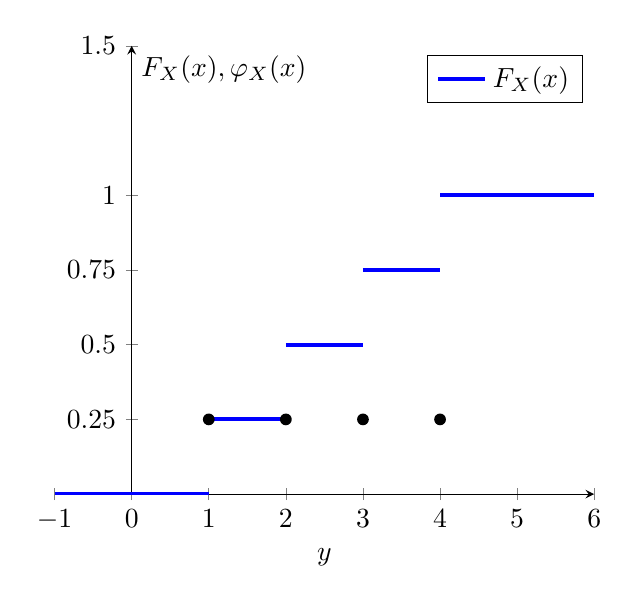
\begin{tikzpicture}
	\begin{axis}[
		axis lines=left,
		axis lines = left,
		xlabel = $y$,
		ylabel = {$F_X(x), \varphi_X(x)$},
		axis y line = middle,
		ymax = 1.5,
		ytick={0, 0.25, 0.5, 0.75, 1, 1.5},
	]
	\addplot [
		domain = -1:1,
		samples = 10, 
		color = blue,
		line width = 1.5pt
	]
	{(x < 1) * 0};
	\addplot [
		domain = 1:2,
		samples = 10, 
		color = blue,
		line width = 1.5pt
	]
	{((x >= 1) && (x < 2)) * 0.25};
	\addplot [
		domain = 2:3,
		samples = 10, 
		color = blue,
		line width = 1.5pt
	]
	{((x >= 2) && (x < 3)) * 0.5};
	\addplot [
		domain = 3:4,
		samples = 10, 
		color = blue,
		line width = 1.5pt
	]
	{((x >= 3) && (x < 4)) * 0.75};
	\addplot [
		domain = 4:6,
		samples = 10, 
		color = blue,
		line width = 1.5pt
	]
	{(x >= 1) * 1};
	{(1,0.25)};
	\node[circle,fill,inner sep=1.5pt] at (axis cs:1,0.25) {};
	\node[circle,fill,inner sep=1.5pt] at (axis cs:2,0.25) {};
	\node[circle,fill,inner sep=1.5pt] at (axis cs:3,0.25) {};
	\node[circle,fill,inner sep=1.5pt] at (axis cs:4,0.25) {};
	\addlegendentry{$F_X(x)$}
	\end{axis}
\end{tikzpicture}
\end{center}

Ma come sono definite le funzioni di \emph{massa} e \emph{ripartizione} di
$Y=2\cdot X+3$?
\[\varphi_Y(y)=P(Y=y)=P(2\cdot X+3=y)=P\left(X=\frac{y-3}{2}\right)=\varphi_X\left(
\frac{y-3}{2}\right)\]
\[F_Y(y)=P(Y\leq y)=P(2\cdot X+3\leq y)=P\left(X\leq \frac{y-3}{2}\right)=F_X\left(
\frac{y-3}{2}\right)\]

\newpage
\paragraph*{Esempio}
Sia $X$ una \emph{variabile aleatoria} uniforme su $[0,1]$ e valga \(Y=2\cdot X+3\).\\
Come cambia $f_Y$?

Sappiamo che \(\int_{-\infty}^{+\infty}f_X(x)dx=\int_{\supp_X}f_X(x)dx=1\),
possiamo quindi aspettarci che anche per Y valga qualcosa del tipo
\(\int_{-\infty}^{+\infty}f_Y(y)dy=\int_{\supp_Y}f_Y(y)dy=c\) per qualche $c\in\R$.
Ma qual è il \emph{supporto di $Y$}?

Il \emph{supporto di $X$} è \(\supp_X=(0,1)\), quindi è ragionevole ipotizzare
che il \emph{supporto di $Y$} sia \(\supp_Y=(3,5)\).

Ora rimane da determinare il valore di $c$. È possibile che $c=1$?
\[c=1=\int_{-\infty}^{+\infty}f_Y(y)dy=\int_{3}^{5}f_Y(y)dy=\int_{3}^{5}1dy=
[y]_{3}^{5}=5-3=2\]
Questa catena di uguaglianze smentisce l'ipotesi che $c=1$ e anzi dimostra
che per questa particolare trasformazione $c=\frac{1}{2}$.

Rimangono ora da definire le \emph{funzioni di massa} e di \emph{ripartizione}:
\[F_Y(y)=P(Y\leq y)=P(2\cdot X+3\leq y)=P\left(X\leq\frac{y-3}{2}\right)=F_X\left(
\frac{y-3}{2}\right)=\]
\[\begin{cases}
	{0} & \text{se}\ {\frac{y-3}{2}<0}\\
	{\frac{y-3}{2}} & \text{se}\ {0\leq\frac{y-3}{2}<1}\\
	{1} & \text{se}\ {\frac{y-3}{2}\geq 1}
\end{cases}=\begin{cases}
	{0} & \text{se}\ {y<0}\\
	{\frac{y-3}{2}} & \text{se}\ {3\leq y<5}\\
	{1} & \text{se}\ {y\geq 5}	
\end{cases}\]
\[f_Y(y)=F'_Y(y)=\begin{cases}
	{0} & \text{se}\ {y\in[3,5]^c}\\
	{\frac{1}{2}} & \text{se}\ {y\in[3,5]}
\end{cases}\]

\begin{center}
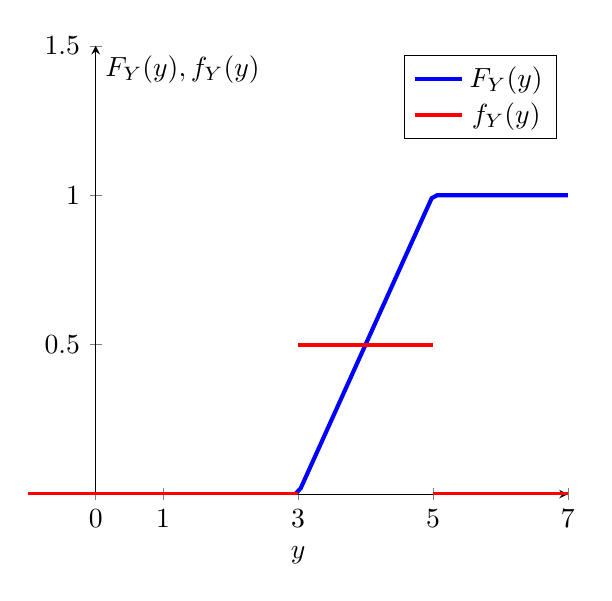
\begin{tikzpicture}
	\begin{axis}[
		axis lines=left,
		axis lines = left,
		xlabel = $y$,
		ylabel = {$F_Y(y), f_Y(y)$},
		axis y line = middle,
		ymax = 1.5,
		xtick={0,1,3,5,7},
	]
	\addplot [
		domain = -1:7,
		samples = 100,
		color = blue,
		line width = 1.5pt
	]
	{(x < 3) * 0 + ((x >= 3) && (x < 5)) * (x - 3) / 2 + (x >= 5) * 1};
	\addlegendentry{$F_Y(y)$}
	\addplot [
		domain = -1:3,
		samples = 10,
		color = red,
		line width = 1.5pt
	]
	{(x < 3) * 0};
	\addlegendentry{$f_Y(y)$}
	\addplot [
		domain = 3:5,
		samples = 10,
		color = red,
		line width = 1.5pt
	]
	{((x >= 3) && (x < 5)) * 0.5};
	\addplot [
		domain = 5:7,
		samples = 10,
		color = red,
		line width = 1.5pt
	]
	{(x >= 5) * 0};

	\end{axis}
\end{tikzpicture}
\end{center}

\begin{proposition}
	Sia $X$ una \emph{variabile aleatoria} e $Y$ una sua trasformazione lineare
	tale che:
	\[Y=a\cdot X+b,\ a,b\in\R\ a\neq 0\]
	La funzione è così definita:
	\[F_Y(y)=\begin{cases}
		{F_X\left(\frac{y-b}{a}\right)} & \text{se}\ {a>0}\\
		{1-F_X\left(\frac{y-b}{a}\right)} & \text{se}\ {a<0\wedge X\ \text{è continua}}\\
		{1-F_X\left(\frac{y-b}{a}\right)+\varphi_X\left(\frac{y-b}{a}\right)} & 
		\text{se}\ {a<0\wedge X\ \text{è discreta}}
	\end{cases}\]
	Inoltre, se $X$ è \emph{assolutamente continua} la \emph{funzione di densità}
	è:
	\[f_Y(y)=\frac{1}{|a|}\cdot f_X\left(\frac{y-b}{a}\right)\]
	Mentre, se $X$ è \emph{discreta} la \emph{funzione di massa} è:
	\[\varphi_Y(y)=\varphi_X\left(\frac{y-b}{a}\right)\]
\end{proposition}
\begin{demonstration}
	\mbox{}\\
	\textbf{Funzione di ripartizione}
	\[F_Y(y)=P(Y\leq y)=P(a\cdot X+b\leq y)=P(A\cdot X\leq y-b)=\cdot \]
	\[\text{Se $a>0$}\ \cdot =P\left(X\leq\frac{y-b}{a}\right)=F_X\left(\frac{y-b}{a}\right)\]
	\[\text{Se $a<0$}\ \cdot =P\left(X\geq\frac{y-b}{a}\right)=1-P\left(X<\frac{y-b}{a}
	\right)=1-\lim_{x\rightarrow(\frac{y-b}{a})^-}F_X(x)=\]
	\[\begin{cases}
		{1-F_X\left(\frac{y-b}{a}\right)} & \text{se $X$ è continua}\\
		{1-F_X\left(\frac{y-b}{a}\right)+P\left(X=\frac{y-b}{a}\right)=1-F_X
		\left(\frac{y-b}{a}\right)+\varphi_X\left(\frac{y-b}{a}\right)} & \text{se
		$X$ è discreta}
	\end{cases}\]

	\noindent
	\textbf{Funzione di densità}
	Se $X$ è \emph{continua} \(f_X=F'_X\), quindi $f_Y$ vale:
	\[f_Y(y)=\frac{d}{dy}F_Y(y)=\begin{cases}
		{\frac{d}{dy}F_X\left(\frac{y-b}{a}\right)} & \text{se}\ {a>0}\\
		{\frac{d}{dy}\left(1-F_X\left(\frac{y-b}{a}\right)\right)} & \text{se}\ {a>0}
	\end{cases}=\begin{cases}
		{F'_X\left(\frac{y-b}{a}\right)\cdot \frac{1}{a}} & \text{se}\ {a>0}\\
		{-F'_X\left(\frac{y-b}{a}\right)\cdot \frac{1}{a}} & \text{se}\ {a<0}
	\end{cases}\]

	A questo punto si può notare che se $a<0$ è possibile semplificare i due $-$
	e ottenere:
	\[f_Y(y)=\frac{1}{|a|}\cdot F'_X\left(\frac{y-b}{a}\right)\]

	\noindent
	\textbf{Funzione di massa}
	Se $X$ è \emph{discreta} abbiamo:
	\[\varphi_Y(y)=P(Y=y)=P(a\cdot X+b=y)=P\left(X=\frac{y-b}{a}\right)=\varphi_Y
	\left(\frac{y-b}{a}\right)\]
\end{demonstration}

\section{Trasformazioni non lineari}
Sia $X$ una \emph{variabile aleatoria} con legge $F_X$ e, con \emph{densità
discreta} $\varphi_X$ se $X$ \emph{v.a. discreta}, o \emph{denstià} $f_X$ se
\emph{v.a. continua}. Sia poi $g:\R\rightarrow\R$ una funzione generica. Come si
definisce la legge di \(Y=g(X)\)?
\begin{note}
	La funzione $g$ non è necessariamente iniettiva o suriettiva.
\end{note}
\subsection{Variabili aleatorie discrete}
Se $X$ è una \emph{variabile aleatoria discreta} possiamo definire la sua funzione
di massa come segue:
\[\varphi_Y(y)=\sum_{x\in g^{-1}(\{y\})}\varphi_X(x)\]

Il \emph{supporto} di $Y$ è \(\supp_Y=g(\supp_X)\) e la \emph{funzione di
ripartizione} si ottiene sommando le $\varphi_Y$:
\[F_Y(y)=\sum_{y\in\supp_Y}\one_{(-\infty, y)}\cdot \varphi_Y(y)\]

\subsection{Variabili aleatorie assolutamente continue}
Se $X$ è una \emph{variabile aleatoria assolutamente continua} un possibile modo
per ricavare la legge di \(Y=g(X)\) è quello di usare la forma di $X$, cioè di $F_X$,
e della funzione $g$.

\paragraph*{Esempio}
Sia $X$ una \emph{variabile aleatoria assolutamente continua} di \emph{densità}:
\[f_X(x)=\begin{cases}
	{e^{-x}} & \text{se}\ {x>0}\\
	{0} & \text{se}\ {x\leq 0}
\end{cases}\]
Se \(g:\R\rightarrow\R\) è definita come \(g=e^{-x}\), qual è la legge di \(Y=e^{-X}\)?

Inizio studiando $X$ per ricavarne la legge.
\[F_X(x)=\int_{-\infty}^{x}f_X(t)dt=\int_{0}^{x}f_X(t)dt=\int_{0}^{x}e^{-t}dt=
[-e^{-t}]_{0}^{x}=1-e^{-x}\Rightarrow\begin{cases}
	{0} & \text{se}\ {x\leq 0}\\
	{1-e^{-x}} & \text{se}\ {x>0}
\end{cases}\]

A questo punto posso passare allo studio di $Y$:
\[F_Y(y)=P(Y\leq y)=P(e^{-X}\leq y)=P(-X\leq \ln(y))\Rightarrow\begin{cases}
	{0} & \text{se}\ {y\leq 0}\\
	{P(-X\leq\ln(y))} & \text{se}\ {y>0}
\end{cases}\Rightarrow\]
\[\begin{cases}
	{0} & \text{se}\ {x\leq 0}\\
	{P(X\geq\ln(y))}\ \text{se} & {0<x<1}\\
	{1} & \text{se}\ {x\geq 1}
\end{cases}=\begin{cases}
	{0} & \text{se}\ {x\leq 0}\\
	{1-F_X(\ln(y))} & \text{se}\ {0<x<1}\\
	{1} & \text{se}\ {x\geq 1}
\end{cases}=\]
\[\begin{cases}
	{0} & \text{se}\ {x\leq 0}\\
	{1-(1-e^{-(\ln(y))})} & \text{se}\ {0<x<1}\\
	{1} & \text{se}\ {x\geq 1}
\end{cases}=\begin{cases}
	{0} & \text{se}\ {x\leq 0}\\
	{y} & \text{se}\ {0<x<1}\\
	{1} & \text{se}\ {x\geq 1}
\end{cases}\]

\begin{observation}
	In questo caso $Y$ è una \emph{variabile aleatoria} uniforme su $[0,1]$.
\end{observation}

Ora che abbiamo la legge di $Y$ possiamo anche ricavarne la \emph{densità} $f_Y$:
\[f_Y(y)=F'_Y(y)=\frac{d}{dy}(1-f_X(-\ln(y)))=-F'_X(-\ln(y))\cdot \frac{d}{dy}(-\ln(y))
=-f_X(-\ln(y))=\]
\[\frac{1}{y}\cdot e^{-(-\ln(y))}\ \text{se}\ {\ln(y)<0}\Rightarrow\begin{cases}
	{0} & \text{se}\ {y\notin(0,1)}\\
	{\frac{1}{y}\cdot y} & \text{se}\ {y\in(0,1)}
\end{cases}\]

Da questa forma è facile passare alla forma della \emph{densità} unforme su $[0,1]$:
\[f_Y(y)=\begin{cases}
	{0} & \text{se}\ {y<0}\\
	{1} & \text{se}\ {0<y<1}\\
	{0} & \text{se}\ {y>1}
\end{cases}\]

\newpage
\paragraph*{Esempio}
Sia $X$ una \emph{varibile aleatoria assolutamente continua} con \emph{funzione
di densità}:
\[f_X(x)=\begin{cases}
	{0} & \text{se}\ {x\leq 0}\\
	{e^{-x}} & \text{se}\ {x>0}
\end{cases}\]
Sia poi, \(Z=g(x)=(1-x)^2\). Qual è la legge di $Z$?

Inizio definendo la \emph{funzione di ripartizione} di $X$:
\[F_X(x)=\int_{-\infty}^{x}f_X(t)dt=\int_{0}^{x}e^{-x}=[-e^{-t}]_{o}^{x}=1-e^{-x}
\Rightarrow\begin{cases}
	{0} & \text{se}\ {x\leq 0}\\
	{1-e^{-x}} & \text{se}\ {x>0}
\end{cases}\]

Passo, ora, allo studio di $Z$:
\[F_Z(z)=P(Z\leq z)=P((1-x)^2\leq z)=\begin{cases}
	{0} & \text{se}\ {x<0}\\
	{P((1-x)^2\leq z)} & \text{se}\ {x\geq 0}
\end{cases}\Rightarrow\]
\[P(|1-x|\leq\sqrt{z})=P(-\sqrt{z}\leq 1-x\leq\sqrt{z})=
P(-1-\sqrt{z}\leq -x\leq -1+\sqrt{z})=\]
\[P(1+\sqrt{z}\geq x\geq 1-\sqrt{z})=F_X(1+\sqrt{z})-F_X(1-\sqrt{z})=\]
\[(1-e^{-(1+\sqrt{z})})\cdot \one_{1+\sqrt{z}>0}-(1-e^{(1-\sqrt{z})})\cdot 
\one_{1-\sqrt{z}>0}\Rightarrow\]
\[F_Z(z)=\begin{cases}
	{0} & \text{se}\ {x<0}\\
	{e^{-(1-\sqrt{z})}-e^{-(1+\sqrt{z})}} & \text{se}\ {0\leq z<1}\\
	{1-e^{-(1+\sqrt{z})}} & \text{se}\ {z\geq 1}
\end{cases}\]

Adesso, posso ricavare la \emph{densità} $f_Z$:
\[f_Z(z)=F'_Z(z)=\frac{d}{dz}(e^{-(1-\sqrt{z})}-e^{-(1+\sqrt{z})})=f_X(1+\sqrt{z})
\cdot \frac{d}{dz}(1+\sqrt{z})-f_X(1-\sqrt{z})\cdot \frac{d}{dz}(1-\sqrt{z})=\]
\[\frac{1}{2\cdot \sqrt{z}}\cdot (f_X(1+\sqrt{z}) + f_X(1-\sqrt{z}))\Rightarrow\]
\[f_Z(z)=\begin{cases}
	{0} & \text{se}\ {z<0}\\
	{\frac{1}{2\cdot \sqrt{z}}\cdot (e^{-(1+\sqrt{z})}+e^{-(1-\sqrt{z})})} & \text{se}\ {0<z<1}\\
	{\frac{1}{2\cdot \sqrt{z}}\cdot e^{-(1+\sqrt{z})}} & \text{se}\ {z<1}
\end{cases}\]

\begin{observation}
	Questo metodo è particolarmente vantaggioso nel caso in cui la \emph{variabile}
	$X$ e la funzione $g$ abbiano buone proprietà, ma la costruzione va "inventata"
	ogni volta, per cui è facile sbagliare.
\end{observation}

\subsubsection{Teorema del cambio di variabile}
Un altro modo per ricavare la legge di \(Y=g(X)\) sfrutta il \emph{Teorema del
cambio di variabile}.
\begin{theorem}[Teorema del cambio di variabile]
	Sia $X$ una \emph{variabile aleatoria assolutamente continua} di \emph{densità}
	$f_X$. Valga poi, \(Y=g(x)\) con \(g:\R\rightarrow\R\), continua a tratti e
	tale per cui \(P(g(x)=0)=0\). Allora
	\[f_Y(y)=\sum_{x\in g^{-1}(\{y\})}\frac{f_X(x)}{|g'(x)|}\]
\end{theorem}

\begin{observation}
	Cosa significa \(P(g(x)=0)=0?\)
	\[\{g'(x)=0\}=\{\omega\in\Omega:g'(X(\omega)=0)\}=\bigcup_{x:g(x)=0}\{\omega
	\in\Omega:\omega\in X^{-1}(\{x\})\}\]
\end{observation}
\begin{observation}
	Perchè si calcola una somma invece di un integrale?
	
	Poiché \(x\in g^{-1}(\{y\})=\{x:g(x)=y\}\), siccome
	\(g'(x)=0\) in un numero al più numerabile di punti, l'insieme \(\{x\in
	g^{-1}(\{y\})\}\) ha al più un numero numerabile di elementi, quindi è
	possibile fare una somma.
\end{observation}

\paragraph*{Esempio}
Siano $X$ come negli esempi precedenti, \(g(x)=(1-x)^2\) e \(Z=g(X)\).

La derivata di $g(x)$ \(g'(x)=-2\cdot (1-x)=2\cdot (x-1)\) si annulla solo in $x=1$. Vediamo
\(g^{-1}(\{z\})\) al variare di \(z\in\R\):
\[g^{-1}(\{z\})=\begin{cases}
	{\emptyset} & \text{se}\ {x<0}\\
	{\{1\}} & \text{se}\ {z=0}\\
	{\{1-\sqrt{z}, 1+\sqrt{z}\}} & \text{se}\ {z>0}
\end{cases}\]

A questo punto, possiamo definire $f_Z$:
\[f_Z(z)=\begin{cases}
	{0} & \text{se}\ {z<0}\\
	{\frac{f_X(1)}{|g'{1}|}} & \text{se}\ {z=0}\\
	{\frac{f_X(1+\sqrt{z})}{g'(1+\sqrt{z})}+\frac{f_X(1-\sqrt{z})}{|g'(1-\sqrt{z})|}} & 
	\text{se}\ {0<z<1}\\
	{\frac{f_X(1+\sqrt{z})}{g'(1+\sqrt{z})}} & \text{se}\ {z>1}
\end{cases}=\begin{cases}
	{0} & \text{se}\ {z<0}\\
	{\frac{e^{-(1+\sqrt{z})}}{2\cdot \sqrt{z}}+\frac{e^{-(1+\sqrt{z})}}{2\cdot \sqrt{z}}} &
	\text{se}\ {0<x<1}\\
	{\frac{e^{-(1+\sqrt{z})}}{2\cdot \sqrt{z}}} & \text{se}\ {z>1}
\end{cases}\]

\begin{center}
\begin{tikzpicture}
	\begin{axis}[
		axis lines=left,
		axis lines = left,
		axis y line = middle,
		xlabel = $z$,
		ylabel = {$\varphi_Z(z)$},
		ymax = 1.5,
	]
	\addplot[
		domain = -1:-0.01,
		samples = 10,
		color = blue,
		line width = 1.5pt
	]
	{(x < 0) * 0};
	\addplot[
		domain = 0.01:0.99,
		samples = 100,
		color = blue,
		line width = 1.5pt
	]
	{((x>0) && (x<1)) * (e^(-(1+x^(0.5)))/(2*x^(0.5))+e^(-(1-x^(0.5)))/(2*x^(0.5)))};
	\addplot[
		domain = 1.01:2,
		samples = 100,
		color = blue,
		line width = 1.5pt
	]
	{(x > 1) * (e^(-(1+x^(0.5)))/(2*x^(0.5)))};
	
	\end{axis}
\end{tikzpicture}
\end{center}

\chapter{Vettori aleatori}

\section{Coppie di variabili aleatorie}
Dato uno spazio di probabilità $\probspace$ si considerino due \emph{
variabili aleatorie} \(X,Y:\Omega\rightarrow\R\). Come si calcola la probabilità
di eventi che coinvolgono entrambe le \emph{variabili aleatorie}? Ad esempio \(
P(X\leq Y)?\) Dobbiamo considerare le coppie \((X,Y):\Omega\rightarrow\R^2\).

\begin{definition}
	Dati, uno spazio di probabilità $\probspace$ e $X,Y$ \emph{variabili aleatorie}
	su di esso si chiama \emph{coppia di variabili aleatorie}, \emph{variabile
	aleatoria doppia} o \emph{2-vettore aleatorio}, la funzione:
	\[V:\Omega\rightarrow\R^2\ t.c.\ V(\omega)=(X(\omega), Y(\omega))\]
	Il \emph{supporto} del \emph{vettore aleatorio} $V$ è definito come:
	\[\supp_V=\supp_{X,Y}=\supp_X\times\supp_Y=\{(X,Y)\in\R^2:x\in\supp_X,
	y\in\supp_Y\}\]
\end{definition}
\begin{definition}
	Sia $(X,Y)$ una \emph{coppia di variabili aleatorie} definite sullo
	stesso spazio di probabilità, la sua \emph{funzione di probabilità} è:
	\[F_{X,Y}((X,Y))=F_{X,Y}(x,y)=P(X\leq x, Y\leq y)\]
	$F_{X,Y}$ si chiama anche \emph{funzione di ripartizione congiunta} di $X,Y$.
\end{definition}

\begin{observation}
	Di solito, note $F_X$ e $F_Y$ non è possibile ricavare $F_{X,Y}$.
	
	Viceversa, nota $F_{X,Y}$ possiamo ricavare $F_X$ e $F_Y$, che in questo caso
	prendono il nome di \emph{marginalità}:
	\[F_X(x)=P(X\leq x)=P(X\leq x, \forall Y)=P(X\leq x, Y<+\infty)=
	\lim_{y\rightarrow +\infty}F_{X,Y}(x,y)\]
	\[F_Y(y)=P(Y\leq y)=P(\forall X, Y\leq y)=P(X<+\infty, Y\leq y)=
	\lim_{x\rightarrow +\infty}F_{X,Y}(x,y)\]
\end{observation}

\begin{definition}
	Data $(X,Y)$ \emph{coppia di variabile aleatorie}, chiamiamo \emph{funzione
	di ripartizione} di $X$ condizionata $Y$ la funzione:
	\[F_{X|Y}(x|y)=\frac{F_{X,Y}(x,y)}{F_Y(y)}\]
\end{definition}
\begin{observation}
	\[F_{X|Y}(x,y)=\frac{P(X\leq x, Y\leq y)}{P(Y\leq y)}=P(X\leq x|Y\leq y)\]
\end{observation}

\begin{definition}
	\mbox{}
	\begin{enumerate}[label=(\roman*)]
		\item Dati uno spazio di probabilità $\probspace$ e due sue tribù $\F_1,\F_2\subset\F$,
		$\F_1$ e $\F_2$ sono indipendenti se ogni evento in $\F_1$ è indipendente da
		ogni evento in $\F_2$
		\item Date due \emph{variabili aleatorie} $X,Y$ su $\probspace$, diciamo
		che $X$ e $Y$ sono indipendenti se lo sono le tribù $\sigma(X)$ e $\sigma(Y)$
		da esse generate
	\end{enumerate}
\end{definition}

\begin{proposition}
	$X$ e $Y$ sono indipendenti se e solo se \(\forall(x,y)\in\R^2\ F_{X,Y}(x,y)=
	F_X(x)\cdot F_Y(y)\).
\end{proposition}

\begin{observation}
	Nel caso di \emph{n-vettori aleatori} per verificare l'indipendenza delle
	\emph{n variabili aleatorie} è necessario controllare tutti i possibili
	raggruppamenti.
\end{observation}

\section{Vettori aleatori discreti}
Nei vettori (in realtà stiamo parlando di \emph{2-vettori}) tutte le \emph{variabili
aleatorie} sono \emph{discrete}.

\begin{definition}
	Siano $X,Y$ \emph{variabili aleatorie discrete} su $\probspace$, chiamiamo
	\emph{densità discreta congiunta} la funzione \(\varphi_{X,Y}:\R^2
	\rightarrow[0,1]\) definita come:
	\[\varphi_{X,Y}(x,y)=P(X=x,Y=y)\]
	La densità discreta di $X$ condizionata $Y$ è:
	\[\varphi_{X|Y}(x|y)=\begin{cases}
		{0} & \text{se}\ {y\notin\supp_Y\Leftrightarrow P(Y=y)=0}\\
		{P(X=x|Y=y)} & \text{se}\ {y\in\supp_Y\Leftrightarrow P(Y=y)\neq 0}
	\end{cases}\]
\end{definition}
\begin{observation}
	Valgono le seguenti proprietà:
	\begin{enumerate}[label=(\roman*)]
		\item \(\forall(x,y)\in\R^2\ 0\leq \varphi_{X,Y}(x,y)\leq 1\)
		\item \(\varphi_{X,Y}(x,y)=0\ \forall x\in\supp_X^c\vee\forall y\in\supp_Y^c\)
		\item \(\sum_{x,y\in\R^2}\varphi_{X,Y}(x,y)=\sum_{(x,y)\in\supp_X\times
		\supp_Y}\varphi_{X,Y}(x,y)=1\)
	\end{enumerate}
\end{observation}

\begin{proposition}
	Sia $(X,Y)$ una \emph{coppia di variabili aleatorie discrete}:
	\begin{enumerate}[label=(\roman*)]
		\item \(\forall(x,y)\in\R^2\ F_{X,Y}(x,y)=\sum_{(x,y)\in\supp_X\times
		\supp_Y}\varphi_{X,Y}(\xi,\eta\in\supp_X\times\supp_Y)\varphi_{X,Y}(\xi,\eta)
		\cdot \one_{\xi\leq\eta}\cdot \one_{\eta\leq\xi}\)
		\item \(\varphi_{X,Y}(x,y)=\varphi_{X,Y}(x|y)\cdot \varphi_Y(y)\)
		\item \(\forall x\in\R\ \varphi_X(x)=\sum_{y\in\supp_Y}\varphi_{X,Y}(x,y)\)
		\item $X,Y$ sono indipendenti se e solo se \(\varphi_{X,Y}(x,y)=
		\varphi_X(x)\cdot \varphi_Y(y)\)
		\item $X,Y$ sono indipendenti se e solo se \(\varphi_X(x)=\varphi_{X|Y}
		(x|y)\) e \(\varphi_Y(y)=\varphi_{Y|X}(y|x)\)
	\end{enumerate}
\end{proposition}
\begin{demonstration}
	\mbox{}
	\begin{enumerate}[label=(\roman*)]
		\item Dalle definizioni
		\item Se \(y\notin\supp_Y\) l'identità è verificata da $0=0$\\
		Se \(y\in\supp_Y\ \varphi_{X|Y}(x|y)\cdot \varphi_Y(y)=P(X=x|Y=y)\cdot P(Y=y)=
		\frac{P(X=x,Y=y)}{P(Y=y)}\cdot P(Y=y)=P(X=x,Y=y)=\varphi_{X,Y}(x,y)\)
		\item \(\sum_{y\in\supp_Y}\varphi_{X,Y}(x,y)=\sum_{y\in\supp_Y}\varphi_
		{Y|X}(y|x)\cdot \varphi_X(x)=\varphi_X(x)\cdot \sum_{y\in\supp_Y}\varphi_{Y|X}(y|x)
		=\\\varphi_X(x)\cdot \sum_{y\in\supp_Y}P(Y=y|X=x)=\varphi_X(x)\cdot 1=\varphi_X(x)\)
		\item $[\Rightarrow]$ dalle definizioni\\
		$[\Leftarrow]$ uso la i e l'analogo risultato visto per le funzioni di
		ripartizione
		\item Segue da $ii$ e $iv$
	\end{enumerate}
\end{demonstration}

\paragraph*{Esempio}
Siano $X,Y$ \emph{variabili aleatorie discrete}. $X$ è il lancio
di una moneta bilanciata:
\[Y=\begin{cases}
	"\text{Lancio di un d6}" & \text{se}\ {X=0}\\
	"\text{Lancio di un d8}" & \text{se}\ {X=1}
\end{cases}\]
Qual è la legge di $Y$?
\[\varphi_{Y|X}(y|x=0)=\begin{cases}
	{0} & \text{se}\ {y\notin\{1,..,6\}}\\
	{\frac{1}{6}} & \text{se}\ {y\in\{1,..,6\}}
\end{cases},\ \varphi_{Y|X}(y|x=1)=\begin{cases}
	{0} & \text{se}\ {y\notin\{1,..,8\}}\\
	{\frac{1}{8}} & \text{se}\ {y\in\{1,..,8\}}
\end{cases}\]
\[\Rightarrow\varphi_{Y|X}(y|x)=\begin{cases}
	{\frac{1}{6}} & \text{se}\ {x=0\wedge y\in\{1,..,6\}}\\
	{\frac{1}{8}} & \text{se}\ {x=1\wedge y\in\{1,..,8\}}\\
	{0} & \text{altrimenti}
\end{cases}\]
Possiamo ricavare \(\varphi_{X,Y}(x,y)=\varphi_{Y|X}(y|x)\cdot \varphi_X(x)\)
\[\varphi_{X,Y}(x,y)=\begin{cases}
	{\frac{1}{6}\cdot \frac{1}{2}} & \text{se}\ {x=0\wedge y\in\{1,..,6\}}\\
	{\frac{1}{8}\cdot \frac{1}{2}} & \text{se}\ {x=1\wedge y\in\{1,..,8\}}\\
	{0} & \text{altrimenti}
\end{cases}=\begin{cases}
	{\frac{1}{12}} & \text{se}\ {x=0\wedge y\in\{1,..,6\}}\\
	{\frac{1}{16}} & \text{se}\ {x=1\wedge y\in\{1,..,8\}}\\
	{0} & \text{altrimenti}
\end{cases}\]
Ora possiamo definire $\varphi_Y(y)$:
\[\varphi_Y(y)=\sum_{x\in\supp_X}\varphi_{X,Y}(x,y)=\begin{cases}
	{\frac{1}{12}+\frac{1}{16}} & \text{se}\ {y\in\{1,..,6\}}\\
	{\frac{1}{16}} & \text{se}\ {y\in\{1,..,8\}}\\
	{0} & \text{altrimenti}
\end{cases}=\begin{cases}
	{\frac{7}{48}} & \text{se}\ {y\in\{1,..,6\}}\\
	{\frac{1}{16}} & \text{se}\ {y\in\{7,8\}}\\
	{0} & \text{altrimenti}
\end{cases}\]
Controlliamo se sono indipendenti:
\[\varphi_X(x)\cdot \varphi_Y(y)=\begin{cases}
	{\frac{7}{48}\cdot \frac{1}{2}} & \text{se}\ {x=0\wedge y\in\{1,..,6\}}\\
	{\frac{7}{48}\cdot \frac{1}{2}} & \text{se}\ {x=1\wedge y\in\{1,..,6\}}\\
	{\frac{1}{16}\cdot \frac{1}{2}} & \text{se}\ {x=1\wedge y\in\{7,8\}}\\
	{0} & \text{altrimenti}
\end{cases}=\begin{cases}
	{\frac{7}{96}} & \text{se}\ {x=0\wedge y\in\{1,..,6\}}\\
	{\frac{7}{96}} & \text{se}\ {x=1\wedge y\in\{1,..,6\}}\\
	{\frac{1}{32}} & \text{se}\ {x=1\wedge y\in\{7,8\}}\\
	{0} & \text{altrimenti}
\end{cases}\]
Dunque $X,Y$ non sono tra loro indipendenti, in quanto $\varphi_{X,Y}(x,y)\neq
\varphi_X(x)\cdot \varphi_Y(y)$

\begin{proposition}
	Siano $X,Y$ due \emph{variabili aleatorie discrete} definite sullo stesso
	spazio di probabilità con \emph{densità discreta congiunta} $\varphi_{X,Y}$.
	La loro somma $X+Y$ ha \emph{densità discreta}:
	\[\varphi_{X+Y}(z)=\sum_{x\in\supp_X}\varphi_{X,Y}(x,z-x)\]
\end{proposition}
\begin{demonstration}
	Vale la seguente catena di uguaglianze:
	\[\varphi_{X+Y}(z)=P(X+Y=z)=P\left(\bigcup_{x\in\supp_X}\{X=x,X+Y=z\}\right)=
	P\left(\bigcup_{x\in\supp_X}\{X=x,Y=z-x\}\right)\]
	\[=\sum_{x\in\supp_x}P(X=x,Y=z-x)=\sum_{x\in\supp_X}\varphi_{X,Y}(x,z-x)\]
\end{demonstration}
\begin{observation}
	Se $X$ e $Y$ sono indipendenti, vale:
	\[\varphi_{X+Y}(z)=\sum_{x\in\supp_X}\varphi_X(x)\cdot \varphi_Y(z-x)\]
\end{observation}

\newpage
\paragraph*{Esempio}
Siano $X,Y$ \emph{variabili aleatorie discrete} associate ciascuna ai risultati
del lancio di un dado a 10 facce. Sia $S=X+Y$, qual è la sua legge? Quali sono
$\varphi_{S,X}$ e $\varphi_{S|X}$?

Inizio definendo $\varphi_X(x)$ e $\varphi_Y(y)$:
\[\varphi_X(x)=\varphi_Y(y)=\begin{cases}
	{\frac{1}{10}} & \text{se}\ {x\in\{1,..,10\}}\\
	{0} & \text{altrimenti}
\end{cases}\]

A questo punto $\varphi_S(z)$ è immediato dalla proposizione:
\[\varphi_S(z)=\varphi_{X+Y}(z)=\sum_{x\in\supp_X}\varphi_X(x)\cdot \varphi_Y(z-x)=
\sum_{i=1}^{10}\varphi_X(x)\cdot \varphi_Y(z-x)\Rightarrow\]
\[\varphi_S(z)=\begin{cases}
	{\frac{1}{100}} & \text{se}\ {z=2\vee z=20}\\
	{\frac{2}{100}} & \text{se}\ {z=3\vee z=19}\\
	{\frac{3}{100}} & \text{se}\ {z=4\vee z=20}\\
	\dots\\
	{\frac{11}{100}} & \text{se}\ {z=11}\\
	{0} & \text{altrimenti}
\end{cases}\]

Ora, passo a ricavare $\varphi_{S,X}(z,x)$:
\[\varphi_{S,X}(z,x)=P(S=z,X=x)=(X+Y=z,X=x)=P(Y=z-X,X=x)=\]
\[\varphi_{X,Y}(x,z-x)=\varphi_X(x)\cdot \varphi_Y(z-x)=\begin{cases}
	{\frac{1}{100}} & \text{se}\ {z\in\{2,..,20\}\wedge x\in\{1,..,10\}}\\
	{0} & \text{altrimenti}
\end{cases}\]

Infine:
\[\varphi_{S|X}(z|x)=\frac{\varphi_{S,X}(z,x)}{\varphi_X(x)}=\frac{\varphi_X(x)\cdot 
\varphi_Y(z-x)}{\varphi_X(x)}=\varphi_Y(z-x)\Rightarrow\]
\[\varphi_{S|X}(z|x)=\begin{cases}
	{\frac{1}{10}} & \text{se}\ {x\in\{1,..,10\}\wedge z\in\{x+1,..,x+10\}}\\
	{0} & \text{altrimenti}
\end{cases}\]

\section{Vettori aleatori assolutamente continui}
\begin{definition}
	Siano $X,Y$ \emph{variabili aleatorie assolutamente continue} definite su
	$\probspace$. Chiamiamo densità congiunta di $X$ e $Y$ la funzione \(F_{X,Y}
	:\R^2\rightarrow\R\) tale che:
	\[\forall E\in\B\times\B\ P((X,Y)\in E)=\int\int_E f_{X,Y}(x,y)dx\ dy\]
\end{definition}

\begin{observation}
	\(P((X,Y)\in E)=P(\{\omega\in\Omega:(X(\omega),Y(\omega)\in E)\})\)
\end{observation}
\begin{proposition}
	Siano $X$ e $Y$ due \emph{variabili aleatorie assolutamente continue}. Allora:
	\begin{enumerate}[label=(\roman*)]
		\item \(\forall(x,y)\in\R^2\ F_{X,Y}(x,y)=\int_{-\infty}^{x}
		\int_{-\infty}^{y}f_{X,Y}(s,t)dt\ ds\)
		\item \(\forall(x,y)\in\R^2\) le densità marginali sono:
		\[f_X(x)=\int_{-\infty}^{+\infty}f_{X,Y}(x,t)dt,\ f_Y(y)=\int_{-\infty}^
		{+\infty}f_{X,Y}(s,y)ds\]
		\item $X,Y$ sono indipendenti se e solo se \(\forall(x,y)\in\R^2\ f_{X,Y}
		(x,y)=f_X(y)\cdot f_Y(y)\)
	\end{enumerate}
\end{proposition}
\newpage
\begin{demonstration}
	\mbox{}
	\begin{enumerate}[label=(\roman*)]
		\item Segue dalla definizione di $F_{X,Y}$ con \(E\in(-\infty,x]\times
		(-\infty,x]\).\\
		Possiamo scrivere la (i) anche come: \(\frac{\partial^2}{\partial x\cdot 
		\partial y}\cdot F_{X,Y}(x,y)=f_{X,Y}(x,y)\)
		\item Segue dai teoremi di integrazione
		\item $[\Rightarrow]$ dalle definizioni\\
		$[\Leftarrow]$ segue da (i) più un'analoga proprietà per $F_{X,Y}$
	\end{enumerate}
\end{demonstration}

\begin{observation}
	\mbox{}
	\begin{itemize}
		\item Per ogni \((x,y)\in\R^2\ f_{X,Y}(x,y)\geq 0\) ma non necessariamente
		$\leq 1$
		\item \({\int\int}_{\R^2}f_{X,Y}(x,y)dx\ dy=1\) percui anche in questo
		caso possiamo parlare di \emph{costanti di rinormalizzazione}
	\end{itemize}
\end{observation}

\paragraph*{Esempio}
Siano $X,Y$ due \emph{variabili aleatorie assolutamente continue} e sia così
definita la \emph{funzione di densità congiunta}:
\[f_{X,Y(x,y)}=\begin{cases}
	{e^{-x}} & \text{se}\ {0\leq y\leq x}\\
	{0} & \text{altrimenti}
\end{cases}\]
Qual è $F_X(x)$?

\[f_X(x)=\int_{-\infty}^{+\infty}f_{X,Y}(x,y)dy=\begin{cases}
	{\int_{0}^{x}e^{-x}dy} & \text{se}\ {x>0}\\
	{0} & \text{se}\ {x<0}
\end{cases}=\begin{cases}
	{x\cdot e^{-x}} & \text{se}\ {x>0}\\
	{0} & \text{se}\ {x<0}
\end{cases}\]
e se volessimo $F_X(x)$:
\[F_X(x)=\int_{-\infty}^{x}f_X(t)dt=\begin{cases}
	{\int_{0}^{x}t\cdot e^{-t}dt} & \text{se}\ {x\geq 0}\\
	{0} & \text{se}\ {x<0}
\end{cases}=\begin{cases}
	{1-e^{-x}\cdot (x+1)} & \text{se}\ {x\geq 0}\\
	{0} & \text{se}\ {x<0}
\end{cases}\]
oppure
\[F_X(x)=\lim_{y\rightarrow +\infty}F_{X,Y}(x,y)=\lim_{y\rightarrow +\infty}\int
_{-\infty}^{x}\int_{-\infty}^{y}f_{X,Y}(s,t)dt\ ds=\int_{-\infty}^{x}\int_{-\infty}
^{+\infty}f_{X,Y}(s,t)dt\ ds\]

\begin{definition}
	Siano $X$ e $Y$ due \emph{variabili aleatorie assolutamente continue} sullo
	stesso spazio di probabilità $\probspace$. Chiamiamo \emph{densità di $X$
	condizionata $Y$} la funzione definita come:
	\[f_{X|Y}(x|y)=\begin{cases}
		{\frac{f_{X,Y}(x,y)}{f_Y(y)}} & \text{se}\ {y\in\supp_Y}\\
		{0} & \text{se}\ {y\notin\supp_Y}
	\end{cases}\]
\end{definition}
\begin{observation}
	\(f_{X,Y}(x,y)=f_{X|Y}(x|y)\cdot f_Y(y)=f{Y|X}(y|x)\cdot f_X(x)\)
\end{observation}

\paragraph*{Esempio}
Siano $X,Y$ \emph{variabili aleatorie assolutamente continue} con la seguente
\emph{funzione di densità congiunta}:
\[f_{X,Y}(x,y)=\begin{cases}
	{6e^{-2x}e^{-3y}}\ & \text{se}\ {x,y>0}\\
	{0} & \text{altrimenti}
\end{cases}\]
$X$ e $Y$ sono indipendenti?

Per essere indipendenti deve valere:
\[f_X(x)\cdot f_Y(y)=f_{X,Y}(x,y)\]
quindi, procedo ricercando $f_X(x)$ e $f_Y(y)$:

\[f_X(x)=\int_{-\infty}^{+\infty}f_{X,Y}(x,y)dy=\begin{cases}
	{\int_{0}^{+\infty}6e^{-2x}e^{-3y}dy} & \text{se}\ {x>0}\\
	{0} & \text{se}\ {x\leq 0}
\end{cases}\]
\[=\begin{cases}
	{6e^{-2x}\cdot \int_{0}^{+\infty}e^{-3y}dy} & \text{se}\ {x>0}\\
	{0} & \text{se}\ {x\leq 0}
\end{cases}=\begin{cases}
	{2e^{-2x}} & \text{se}\ {x>0}\\
	{0} & \text{se}\ {x\leq 0}
\end{cases}\]
\[f_Y(y)=\int_{-\infty}^{+\infty}f_{X,Y}(x,y)dx\begin{cases}
	{\int_{0}^{+\infty}6e^{-2x}e^{-3y}dx} & \text{se}\ {y>0}\\
	{0} & \text{se}\ {y\leq 0}
\end{cases}\]
\[=\begin{cases}
	{6e^{-3y}\cdot \int_{0}^{+\infty}e^{-2x}dx} & \text{se}\ {y>0}\\
	{0} & \text{se}\ {y\leq 0}
\end{cases}=\begin{cases}
	{3e^{-3y}} & \text{se}\ {y>0}\\
	{0} & \text{se}\ {y\leq 0}
\end{cases}\]
Ora, verifico la condizione di indipendenza:
\[f_X(x)\cdot f_Y(y)=\begin{cases}
	{2e^{-2x}\cdot 3e^{-3y}} & \text{se}\ {x,y>0}\\
	{0} & \text{altrimenti}
\end{cases}=\begin{cases}
	{6e^{-2x}e^{-3y}} & \text{se}\ {x,y>0}\\
	{0} & \text{altrimenti}
\end{cases}=f_{X,Y}(x,y)\]
Quindi, $X$ e $Y$ sono indipendenti.

\begin{proposition}[Somma di \emph{v.a. assolutamente continue}]
	Siano $X$ e $Y$ \emph{variabili aleatorie assolutamente continue}, definite
	nello stesso spazio di probabilità $\probspace$, con \emph{densità congiunta}
	$f_{X,Y}$. La \emph{variabile aleatoria} $X+Y$ ha \emph{densità}:
	\[f_{X+Y}(z)=\int_{-\infty}^{+\infty}(x,z-x)dx\]
\end{proposition}
\begin{demonstration}
	Consideriamo la \emph{funzione di ripartizione} $F_{X+Y}(z)=P(X+Y\leq z)$.
	Questa probabilità può essere vista come \(P((X,Y)\in E)\) per qualche \(E
	\in\B\times\B\), infatti:
	\[X+Y\leq z\Leftrightarrow Y\leq z-X\]
	Se lo si rappresenta nel piano $\R^2$, questa condizione è verificata da tutti
	i punti al di sotto della retta \(y=-x+z\), quindi:
	\[F_{X,Y}(z)=P((X,Y)\in E)=\int\int_Ef_{X,Y}(x,y)dy\ dx=\int_{-\infty}^
	{+\infty}\int_{-\infty}^{z-x}f_{X,Y}(x,y)dy\ dx\]
	Per ricavare la densità è sufficiente derivare in z.
\end{demonstration}

\section{Vettori aleatori misti}
Per quanto riguarda i \emph{vettori aleatori misti} esamineremo soltanto il caso
dei \emph{vettori} composti da una \emph{variabile aleatoria discreta} e una
\emph{assolutamente continua}.

\paragraph*{Esempio}
All'Università di Trento, gli studenti si dividono tra un 52\% iscritto a materie
umanistiche e un 48\% iscritto a materie scientifiche.
Tra chi studia materie scientifiche il tempo di studio giornaliero è uniformemente
distribuito tra 155 e 180 minuti, mentre per chi studia materie umanistiche il
tempo varia tra 143 e 166 minuti.

Siano $X$ la \emph{variabile aleatoria} che traccia l'ambito di studio degli
studenti, e $Y$ la \emph{variabile aleatoria} che ne indica il tempo di studio
giornaliero.
\begin{enumerate}
	\item Qual è, se esiste, la legge congiunta di $X$ e $Y$?
	\item Qual è la probabilità che un qualunque studente studi al più 160 minuti?
	\item Come sono suddivisi tra i due indirizzi gli studenti che studiano meno
	di 160 minuti?
	\item E come sono distribuiti quelli che studiano esattamente 160 minuti?
\end{enumerate}

Osservo che $X$ è una \emph{variabile aleatoria discreta}, mentre $Y$ è \emph{
assolutamente continua}. Inizio quindi defininendo le \emph{funzioni di densità}
di $X$ e $Y$ condizionata $X$:
\[\varphi_X(x)=\begin{cases}
	{0} & \text{se studia materie scientifiche}\\
	{1} & \text{se studia materie umanistiche}
\end{cases}\]
\[f_{Y|X}(y|0)=\begin{cases}
	{cs} & \text{se}\ {y\in[155,180]}\\
	{0} & \text{altrimenti}
\end{cases};\ f_{Y|X}(y|1)=\begin{cases}
	{cu} & \text{se}\ {y\in[143,166]}\\
	{0} & \text{altrimenti}
\end{cases}\]
Devo trovare i valori delle costanti $cs$ e $cu$:
\[\int_{-\infty}^{+\infty}f_{Y|X}(y|0)dy=[cs\cdot y]_{155}^{180}=cs\cdot (180-155)=cs\cdot 25
\Rightarrow cs=\frac{1}{25}\]
\[\int_{-\infty}^{+\infty}f_{Y|X}(y|1)dy=[cu\cdot y]_{143}^{166}=cu\cdot (166-143)=cu\cdot 23
\Rightarrow cu=\frac{1}{23}\]
Da qui è facile definire $f_{Y|X}(y|x)$:
\[f_{Y|X}(y|x)=\begin{cases}
	{\frac{1}{25}} & \text{se}\ {x=0\wedge y\in[155,180]}\\
	{\frac{1}{23}} & \text{se}\ {x=1\wedge y\in[143,166]}\\
	{0} & \text{altrimenti}
\end{cases}\]
A questo punto possiamo ricavare la legge congiunta di $X$ e $Y$:
\[f_{X,Y}(x,y)=f_{Y|X}(y|x)\cdot f_{X}(x)=\begin{cases}
	{\frac{1}{25}\cdot 0.48=0.0192} & \text{se}\ {x=0\wedge y\in[155,180]}\\
	{\frac{1}{23}\cdot 0.52=0.0226087} & \text{se}\ {x=1\wedge y\in[143,166]}\\
	{0} & \text{altrimenti}
\end{cases}\]
Per rispondere al secondo quesito è necessario ricavare $F_Y(y)$. Prima però serve
la \emph{funione di densità} di $Y$. Per farlo marginalizziamo $f_{X,Y}$ sommando
tutti i 2 valori di $X$:
\[f_Y(y)=f_{X,Y}(0,y)+f_{X,Y}(1,y)=\begin{cases}
	{0.0226087} & \text{se}\ {y\in[143,155)}\\
	{0.0226087+0.0192=0.0418087} & \text{se}\ {y\in[155,166)}\\
	{0.0192} & \text{se}\ {y\in[166,180]}\\
	{0} & \text{altrimenti}
\end{cases}\]
Ora, ricaviamo $F_Y(y)$:
\[F_Y(y)=\begin{cases}
	{0} & \text{se}\ {y < 143}\\
	{0.0226087\cdot (y-143)} & \text{se}\ {143\leq y < 155}\\
	{0.0418087\cdot (y-155)+0.2713044} & \text{se} \ {155\leq y <166}\\
	{0.0192\cdot (y-166)+0.7312001} & \text{se}\ {166\leq y<180}\\
	{1} & \text{se}\ {x\geq 180}
\end{cases}\]
\begin{note}
	Le costanti $0.2713044$ e $0.7312001$ sono state calcolate come segue:
	\begin{itemize}
		\item \(0.2713044=0.0226087\cdot (155-143)\)
		\item \(0.7312001=0.0418087\cdot (166-155)+0.2713044\)
	\end{itemize}
	Anche l'uno può essere ottenuto allo stesso modo, infatti: \(1=0.0192\cdot 
	(180-166)+0.7312001\).
\end{note}

\begin{center}
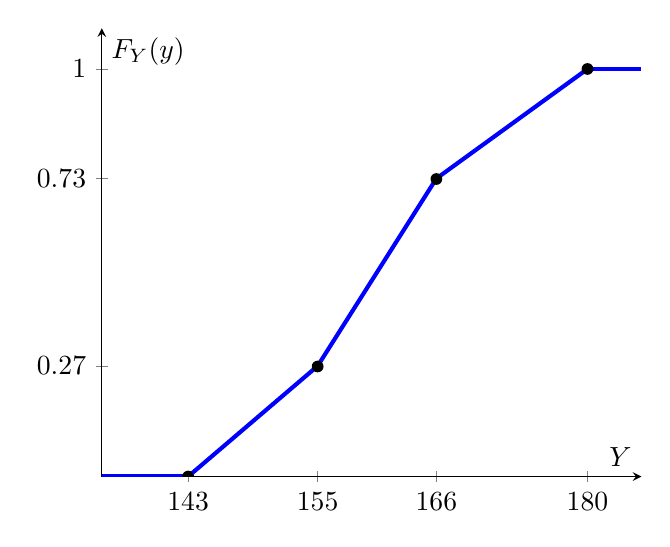
\begin{tikzpicture}
	\begin{axis}[
		axis lines = center,
		xlabel=$Y$,
		ylabel=$F_Y(y)$,
		ytick = {0, 0.2713044, 0.7312001, 1},
		xtick = {143, 155, 166, 180},
		xmin = 135,
		ymax = 1.1
	],
	\addplot[
		domain = 0:143,
		samples = 10,
		color = blue,
		line width = 1.5pt
	]{(x<143) * 0};
	\addplot[
		domain = 143:155,
		samples = 100,
		color = blue, 
		line width = 1.5pt
	]{((x >= 143) && (x < 155)) * (0.0226087 * (x-143))};
	\addplot[
		domain = 155:166,
		samples = 100,
		color = blue,
		line width = 1.5pt
	]{((x >= 155) && (x < 166)) * (0.2713044 + 0.0418087 * (x-155))};
	\addplot[
		domain = 166:180,
		samples = 100,
		color = blue,
		line width = 1.5pt
	]{((x >= 166) && (x < 180)) * (0.7312001 + 0.0192 * (x-166))};
	\addplot[
		domain = 180:185,
		samples = 10,
		color = blue,
		line width = 1.5pt
	]{(x >= 180) * 1};

	\node[circle,fill,inner sep=1.5pt] at (axis cs:143,0) {};
	\node[circle,fill,inner sep=1.5pt] at (axis cs:155,0.27) {};
	\node[circle,fill,inner sep=1.5pt] at (axis cs:166,0.73) {};
	\node[circle,fill,inner sep=1.5pt] at (axis cs:180,1) {};
		
	\end{axis}
\end{tikzpicture}
\end{center}
A questo punto, per rispondere al secondo quesito, basta calcolare $F_Y(160)$:
\[F_Y(160)=P(Y\leq 160)=0.0418087\cdot (160-155)+0.2713044\approx 0.48\]
Al terzo quesito si risponde calcolando la probabilità di $X$ condizionata $Y$:
\[P(X=x|Y<160)=\frac{P(X=x, Y<160)}{P(Y<160)}=\frac{\int_{143}^{160}f_{X,Y}(x,y)dy}
{F_Y(160)}=\]
\[\begin{cases}
	{\frac{[0.0192\cdot y]_{155}^{160}}{0.48}\approx 0.20} & \text{se}\ {X=0}\\
	{\frac{[0.0226087\cdot y]_{143}^{160}}{0.48}\approx 0.80} & \text{se}\ {X=1}
\end{cases}=\begin{cases}
	{20\%} & \text{studia materie scientifiche}\\
	{80\%} & \text{studia materie umanistiche}
\end{cases}\]
Per il quarto quesito non si può calcolare $P(X=x,y=160)$ perchè la probabilità
di un punto è 0, quindi calcoliamo:
\[f_{X|Y}(x|160)=\frac{f_{X,Y}(x,160)}{f_Y(160)}=\begin{cases}
	{\frac{0.0192}{0.0418087}} & \text{se}\ {x=0}\\
	{\frac{0.0226087}{0.0418087}} & \text{se}\ {x=1}
\end{cases}\approx\begin{cases}
	{0.46} & \text{se}\ {x=0}\\
	{0.54} & \text{se}\ {x=1}
\end{cases}\]

\chapter{Modelli di variabili aleatorie discrete}

\section{Bernoulliane}
\begin{definition}
	Una \emph{variabile aleatoria} si dice \emph{Bernoulliana} di paramentro
	$p\in[0,1]$, e indicheremo in simboli \(X\sim bin(1,p)\), se ha
	\emph{densità discreta}:
	\[\varphi_X(x)=\begin{cases}
		{p} & \text{se}\ {x=1}\\
		{1-p} & \text{se}\ {x=0}\\
		{0} & \text{altrimenti}
	\end{cases}\]
	La \emph{funzione di ripartizione} di una \emph{Bernoulliana} di parametro
	$p$	è:
	\[F_X(x)=\begin{cases}
		{0} & \text{se}\ {x<0}\\
		{1-p} & \text{se}\ {0\leq x<1}\\
		{1} & \text{se}\ {x\geq 1}
	\end{cases}\]
\end{definition}
\begin{observation}
	È una \emph{variabile aleatoria indicatrice} in cui $E="successo"$.
\end{observation}

\section{Binomiali}
Ipotiziamo di avere $n$ \emph{variabili aleatorie Bernoulliane} di parametro $p$
indipendenti (ad esempio $n$ lancio di una moneta bilanciata). Se ne prendiamo
la somma $S$, $S$ indica il numero di successi.

\begin{definition}
	Sia $X$ una \emph{variabile aleatoria discreta binomiale} di $n$ parametri
	$p\in[0,1]$ con \(n\in\N\symbol{92}\{0\}\). Se $X$ è definita come la somma
	di $n$ \emph{Bernoulliane} di parametro $p$ indipendenti scriveremo \(X\sim
	bin(n,p)\).
\end{definition}
\begin{proposition}
	Se \(X\sim bin(n,p)\) allora \(\varphi_X(k)=\begin{cases}
		{\binom{n}{k}\cdot p^k\cdot (1-p)^{n-k}} & \text{se}\ {k\in\{0,..,n\}}\\
		{0} & \text{altrimenti}
	\end{cases}\)
\end{proposition}

\begin{demonstration}
	Sia \(\supp_X=\{0,..,n\}\) il \emph{supporto} di $X$. Preso \(k\in\supp_X\
	\varphi_X(k)=P(X=k)=P(\sum_{i=1}^nX_i=k)\) con \(X_i\sim bin(1,p)\ \forall i\)
	indipendenti tra loro. Chiamiamo $N=\{1,..,n\}$ l'insieme degli indici delle
	\emph{Bernoulliane} e indichiamo con \(\mathcal{I}_k\subseteq\mathcal{P}(N)\)
	la famiglia dei sottoinsiemi di $N$ con esattamente $k$ elementi:
	\[\mathcal{I}_k=\{I_k\in\mathcal{P}(N):\#I_k=k\}\]
	Per ciascun insieme $I_k$ definiamo:
	\[E_{I_k}=\bigcap_{i\in I_k}\{X_i=1\}\cap\bigcap_{i\in I_k^c}\{X_i=0\}\]
	Preso atto che \(\{X=k\}=\bigcup_{I_k\in\mathcal{I}_k}E_{I_k}\) vale:
	\[P(E_{I_K})=P\left(\bigcap_{i\in I_k}\{X_i=1\}\cap\bigcap_{i\in I_k^c}
	\{X_i=0\}\right)\]
	\[=\prod_{i\in I_k}\cdot P(X_i=1)\cdot \prod_{i\in I_k^c}\cdot P(X_i=0)=p^k\cdot (1-p)^{n-k}\]
	A questo punto la \emph{funzione di massa} è:
	\[\varphi_X(k)=\sum_{I_k\in\mathcal{I}_k}p^k\cdot (1-p)^{n-k}=p^k\cdot (1-p)^{n-k}\cdot 
	\sum_{I_k\in\mathcal{I}_k}1=p^k\cdot (1-p)^{n-k}\cdot \binom{n}{k}\]
\end{demonstration}

\begin{observation}
	La \emph{funzione di ripartizione} è definita come:
	\[F_X(x)=\sum_{k=0}^{\lfloor x\rfloor}\varphi_X(k)=\sum_{k=0}^{min\{\lfloor
	x\rfloor,n\}}\binom{n}{k}\cdot p^k\cdot (1-p)^{n-k}\]
	e in particolar,e se $X\geq 1$ \(F_X(x)=1\), infatti:
	\[\sum_{k=0}^n\binom{n}{k}\cdot p^k\cdot (1-p)^{n-k}=(p+(1-p))^n=1\]
\end{observation}

\paragraph*{Esempio}
Un'azienda produttrice di chiavette USB, produce chiavette difettose con probabilità
del 2\%. Vende le pennette in confezioni da 15 e se in una confezione ce ne sono
almeno due difettose rimborsa il cliente.
\begin{enumerate}
	\item Quale percentuale di confezioni viene rimborsata?
	\item Comprando 4 confezioni con che probabilità esattamente una confezione
	è rimborsabile?
\end{enumerate}

Definisco due \emph{variabili aleatorie}:
\begin{enumerate}[label=(\roman*)]
	\item $O\sim bin(1,0.02)$: indica se una pennetta è difettosa o meno
	\item $N\sim bin(15,0.02)$: conta le pennette difettose in una confezione
\end{enumerate}

Per rispondere al primo quesito, calcolo la probabilità che in una confezione ci
siano più di una pennetta USB difettose:
\[P(N>1)=\sum_{k=2}^{15}P(N=k)=1-P(N=0)-P(N=1)=1-\varphi_N(0)-\varphi_N(1)=\]
\[1-\binom{15}{0}\cdot 0.02^0\cdot (1-0.02)^{15}-\binom{15}{1}\cdot 0.02^1\cdot (1-0.02)^{14}=
1-0.98^{15}-15\cdot 0.02\cdot 0.98^{14}\approx 3.5\%\]

Per rispondere invece, al secondo quesito definisco una nuova \emph{variabile
aleatoria} $S$ che conta il numero di scatole rimborsabili: \(S\sim bin(4,P(N>1)
)=bin(4,0.035)\).
\[\varphi_S(1)=\binom{4}{1}\cdot 0.035^1\cdot (1-0.035)^3\approx 12.7\%\]

\subsection{Bernoulliane e binomiali in R}
Presa una \emph{binomiale} la \emph{funzione di densità discreta} è la funzione:
\begin{center}
	\texttt{dbinom(x, size, prob)}
\end{center}
dove \texttt{x} è il punto in cui vogliamo calcolare la \emph{densità} $\varphi$,
\texttt{size} è il numero di tentativi (nella definizione 8.2.1 è stato chiamato
$n$) e \texttt{prob} è la probabilità di successo di ogni tentativo (nella def. 
8.2.1 era $p$).

\paragraph*{Esempio}
Sia $X\sim bin(44, 0.2)$ una \emph{binomiale}. Qual è la probabilità di
$\varphi_X(11)$?
\begin{center}
	$\varphi_X(11)$ = \texttt{dbinom(x = 11, size = 44, prob = 0.2) =}\\
	\texttt{dbinom(size = 44, x = 11, prob = 0.2) = dbinom(11, 44, 0.2)}
\end{center}

\noindent
La \emph{funzione di ripartizione} è invece la funzione:
\begin{center}
	\texttt{pbinom(q, size, prob, lower.tail = TRUE)}
\end{center}
i cui parametri \texttt{size}, \texttt{prob} sono gli stesso di \texttt{dbinom},
mentre \texttt{q} è il punto in vogliamo calcolare la \emph{funzione di
ripartizione $F_X$} e \texttt{lower.tail} è un parametro logico che che determina
se stiamo calcolando la \emph{funzione di ripartizione} $F_X$ nel punto \texttt{q}
(ossia \(P(X\leq q)\), la "coda inferiore") in corrispondenza del valore 
\texttt{TRUE} o il suo complementare \(1-F_X(q)\) (cioè \(P(X>q)\), la "coda
superiore") in corrispondeza del valore \texttt{FALSE}.

\paragraph*{Esempio}
Sia $X\sim bin(23, 0.5)$ una \emph{binomiale}. Qual è la probabilità di
$\F_X(12.5)$ e \(P(X>10)\)?
\begin{center}
	$F_X(12.5)$ = \texttt{pbinom(q = 12.5, size = 23, prob = 0.5, lower.tail = TRUE) =}\\
	\texttt{dbinom(size = 23, q = 12.5, prob = 0.5)= dbinom(12.5, 23, 0.5)}\\
	$P(X>10)$ = \texttt{pbinom(q = 10, size = 23, prob = 0.5, lower.tail = FALSE) =}\\
	\texttt{dbinom(12.5, 23, 0.5, FALSE)}
\end{center}

Ci sono anche altre funzioni per le \emph{binomiali} in R: \texttt{rbinom} e
\texttt{qbinom}.\\
\texttt{rbinom(n, size, prob)} è un generatore casuale di risultati distribuiti
come una binomiale dei parametri assegnati, cioè genera dei valori \(X(\omega)
\in\R\) con \(X\sim bin(n,p)\). I parametri \texttt{size} e \texttt{prob} sono
gli stessi delle funzioni precedenti, mentre \texttt{n} indica il numero di valori
da generare.\\
\texttt{qbinom} è la funzione \emph{quantile}.

\paragraph*{Esempio}
Se vogliamo un campione di 100 esiti di lanci di una moneta bilanciata, che è una
\emph{Bernoulliana} di parametro \(p=0.5\), possiamo usare:
\begin{center}
	\texttt{rbinom(n = 100, size = 1, prob = 0.5)}
\end{center}

\section{Schema o processo di Bernoulli}
\begin{definition}
	Si definisce \emph{schema} o \emph{processo di Bernoulli} una successione
	infinita di \emph{Bernoulliane} indipendenti e identicamente distribuite:
	\[\{X_i\}_{i\in\N}\ X_i\sim bin(1,p)\]
\end{definition}

Dato uno \emph{schema di Bernoulli} definiamo lo spazio di probabilità $\probspace$
prendendo:
\begin{itemize}
	\item $\Omega=\{0,1\}^\N$, cioè successioni a valori in $\{0,1\}$
	\item Siccome l'universo è uno \emph{spazio prodotto infinito}, come
	\emph{tribù} prendiamo la \emph{tribù} $\F$ generata dai \emph{cilindri}.
	I \emph{cilindri} in questo caso sono i sottoinsiemi \(C\subseteq\Omega\)
	tali che esistono un naturale \(n\in\N\) e un vettore \(v=\{0,1\}^n\):
	\[C=\{\omega\in\Omega : \omega_i = v_i\ \text{per}\ 1\leq i\leq n\}\]
	\item $P$ è il prodotto delle probabilità delle componenti
\end{itemize}

\paragraph*{Esempio}
Sia \(\{X_i\}_{i\in\N}\ X_i\sim bin(1,p)\) uno \emph{schema di Bernoulli}.
\begin{enumerate}
	\item Qual è la probabilità di avere un successo seguito da 2 insuccessi?
	\item E che il primo successo sia al k-esimo tentativo?
	\item E la probabilità che il terzo esito sia un successo?
\end{enumerate}

\begin{enumerate}
	\item Il cilindro corrispondente è:
	\[(1,0,0,*,*,*,\dots)\]
	cioè $n=3$ e $v={1,0,0}$, mentre la probabilità è:
	\[P = p\cdot (1-p)^2\cdot \prod_{i=1}^{+\infty}1=p\cdot (1-p)^2\]
	\item Il cilindro stavolta è:
	\[(0,0,\dots,0,1,*,*,\dots)\]
	con $k-1$ insuccessi e un successo come k-esimo esito. La probabilità diventa:
	\[P=(1-p)^{k-1}\cdot p\cdot \prod_{i=1}^{+\infty}1=(1-p)^{k-1}\cdot p\]
	\item Infine, nel terzo quesito il cilindro è:
	\[(*,*,1,*,*,\dots)\]
	Questo di per sè non sarebbe un cilindro in quanto non inizia con un vettore,
	ma posso posso comunque immaginarlo come unione di cilindri:
	\[(*,*,1,*,*,\dots)=(0,0,1,*,*,\dots)\cup(1,0,1,*,*,\dots)\cup(0,1,1,*,*
	,\dots)\cup(1,1,1,*,*,\dots)\]
	percui, la probabilità si calcola come:
	\[P=P(0,0,1,*)+P(1,0,1,*)+P(0,1,1,*)+P(1,1,1,*)=\]
	\[(1-p)^2\cdot p+p\cdot (1-p)\cdot p+(1-p)\cdot p2+p^3=p\cdot ((1-p)^2+2p
	\cdot (1-p)+p^2)=\]
	\[p\cdot ((1-p)+p)^2=p\]
\end{enumerate}

\section{Geometriche}
Preso uno \emph{schema di Bernoulli} di parametro $p$, siamo interessati al numero
di insuccessi che si verificano prima del primo successo. Definiamo quindi una
\emph{variabile aleatoria} che tracci l'indice del primo successo:
\[T_1=inf\{i\geq 1:\omega_i=1\}\]

Questa particolare \emph{variabile aleatoria} si chiama \emph{tempo di arresto},
ma è anche una \emph{variabile aleatoria indicatrice} dell'istante di primo
successo. Quindi, per ricavare il numero di insuccessi basta considerare $T_1-1$.

\begin{definition}
	Una \emph{variabile aletoria} è una \emph{geometrica} di parametro $p$, e
	scriveremo \(X\sim geom(p)\), se è l'istante precedente al primo successo in
	un \emph{processo di Bernoulli} di parametro $p$.
\end{definition}

\begin{observation}
	Qual è la \emph{funzione di massa} $\varphi_X$ di una \emph{geometrica}?

	\(\varphi_X(k)=P(X=k)\) equivale a chiedere quale sia la probabilità che si
	verifichino $k$ insuccessi prima del primo successo:
	\[\varphi_X(k)=P(X=k)=\begin{cases}
		{0} & \text{se}\ {k\notin\N}\\
		{(1-p)^k\cdot p} & \text{se}\ {k\in\N}
	\end{cases}\]
\end{observation}
\begin{note}
	In alcuni testi la \emph{geometrica} indica l'istante di primo successo ($T_1$)
	invece del numero di insuccessi ($T_1-1$), ma la probabilità risultante è la
	stessa.
\end{note}
\begin{observation}
	\[\sum_{k=0}^{+\infty}\varphi_X(k)=\sum_{k=0}^{+\infty}(1-p)^k\cdot p=p\cdot \sum_{k=0}
	^{+\infty}(1-p)^k=p\cdot \frac{1}{1-(1-p)}=p\cdot \frac{1}{p}=1\]
	\begin{note}
		\(\sum_{k=1}^{+\infty}(1-p)^k\) è una \emph{serie geometrica}. Da qui il
		nome \emph{variabile aleatoria geometrica}.
	\end{note}
\end{observation}

\begin{observation}
	Qual è la \emph{funzione di ripartizione} $F_X$ di una \emph{geometrica}?
	\[F_X(x)=\begin{cases}
		{0} & \text{se}\ {x<0}\\
		{\sum_{k=0}^{\lfloor x\rfloor}\varphi_X(x)} & \text{se}\ {x\geq 0}
	\end{cases}=\begin{cases}
		{0} & \text{se}\ {x<0}\\
		{p\cdot \sum_{k=0}^{\lfloor x\rfloor}(1-p)^k} & \text{se}\ {x\geq 0}
	\end{cases}=\]
	\[\begin{cases}
		{0} & \text{se}\ {x<0}\\
		{p\cdot \frac{1-(1-p)^{\lfloor x\rfloor+1}}{1-(1-p)}} & \text{se}\ {x\geq 0}
	\end{cases}=\begin{cases}
		{0} & \text{se}\ {x<0}\\
		{1-(1-p)^{\lfloor x\rfloor+1}} & \text{se}\ {x\geq 0}
	\end{cases}\]
	\begin{note}
		Avremmo potuto raggiungere in modo più diretto lo stesso risultato,
		considerando il complementare 
	\end{note}
\end{observation}

\begin{proposition}[Assenza di memoria]
	\(\forall n\in\N\ P(X\geq n+k|X\geq n)=P(X\geq k)\)
\end{proposition}
\begin{demonstration}
	\[P(X\geq n+k|X\geq n)=\frac{P((X\geq n+k)\cap(X\geq n))}{P(X\geq n)}=\frac
	{P(X\geq n+k)}{P(X>n-1)}=\]
	\[\frac{PXn+k-1}{P(X>n-1)}=\frac{(1-p)^{n+k-1+1}}{(1-p)^{n-1+1}}=\frac{(1-p)
	^{n+k}}{(1-p)^n}=(1-p)^k=P(X\geq k)\]
\end{demonstration}

\begin{observation}
	Cosa significa \emph{assenza di memoria}?

	La proposizione può essere letta come:
	\enquote{Se dopo $n$ tentantivi non si è verificato alcun successo, possiamo
	iniziare un nuovo \emph{schema di Bernoulli} con uguale parametro e calcolare
	la probabilità che si verifichino almeno k insuccessi prima di un successo.}
	Cioè, sapere quanti insuccessi ci sono stati non ci dà alcuna informazione
	aggiuntiva sull'istante in cui si verificherà il prossimo successo.
\end{observation}

\paragraph*{Esempio}
Nel Superenalotto il 55 non esce da 60 estrazioni.
\begin{enumerate}
	\item Con che probabilità uscirà alla prossima estrazone?
	\item E che esca la prossima volta tra almeno 30 estrazioni?
\end{enumerate}
\begin{enumerate}
	\item Calcolare la probabilità che esca 55 equivale a calcolare la probabilità
	che non esca e considerarne il complementare:
	\[P(\text{"esce 55"})=1-P(\text{"non esce 55"})=1-\frac{\binom{89}{6}}
	{\binom{90}{6}}=\frac{\binom{89}{5}}{\binom{90}{6}}=\frac{6}{90}=\frac{1}{15}
	\approx 6.6\%\]
	
	Avrei potuto rispondere al quesito, anche sfruttando gli \emph{schemi di
	Bernoulli}.\\	
	Sia $X$ la \emph{variabile indicatrice} di "esce 55", \(X\sim bin(1,\frac{1}
	{15})\) uno \emph{schema di Bernoulli} di parametro $\frac{1}{15}$.
	\[P(\text{"55 esce alla $61^a$ estrazione"})=P(X=60|X\geq 60)=\frac{P(X=60)}
	{P(X>59)}=\]
	\[\frac{(1-\frac{1}{15})^{60}\cdot \frac{1}{15}}{(1-\frac{1}{15})^{59+1}}=
	\frac{1}{15}\]

	Si può notare che il risultato è lo stesso del primo quesito. Questo avviene
	per effetto dell'\emph{assenza di memoria}. Infatti, sapere che ci sono stati
	60 insuccessi non influenza la probabilità che se ne verifichi uno.
	\item Utilizzando lo stesso \emph{schema di Bernoulli} si ha:
	\[P(X\geq 60+30|X\geq 60)=P(X\geq 30)=(1-\frac{1}{15})^{30}\approx 12.6\%\]
\end{enumerate}

\subsection{Geometriche in R}
Come per le \emph{Binomiali}, anche per le \emph{geometriche} c'è una famiglia di
funzioni che ne permettono la manipolazione:
\begin{itemize}
	\item \texttt{dgeom(x, prob)}\\
	Questa funzione permette di calcolare la \emph{funzione di massa} nel punto
	\texttt{x}, sapendo che la probabilità di successo, cioè che il parametro
	della \emph{geometrica}, è \texttt{prob}.
	\item \texttt{pgeom(q, prob, lower.tail = TRUE)}\\
	Calcola il valore della \emph{cdf} nel punto \texttt{q}, considerando di nuovo
	come parametro \texttt{prob}. Inoltre, se \texttt{lower.tail = TRUE} calcola
	direttamente la $cdf$, altrimenti ne considera il complementare.
	\item \texttt{rgeom(n, size, prob)}\\
	Genera casualmente \texttt{n} risultati distribuiti come una \emph{geometrica}.
	\item \texttt{qgeom}\\
	È la funzione \emph{quantile}.
\end{itemize}

\section{Binomiali negative}
Si consideri l'istante dell'ennesimo successo di uno \emph{schema di Bernoulli}
\((n\in\N\symbol{92}\{0\})\) e lo si chiami $I_n$. $I_n$ sarà definito come:
\[T_n=inf\{i\geq 1:\sum_{k=1}^i\omega_k=n\}\]
\begin{note}
	$T_n$ è anche definibile in modo ricorsivo, come segue:
	\[\begin{cases}
		T_1=inf\{i\geq 1:\omega_i=1\}\\
		T_{n+1}=inf\{1>T_n:\omega_i=1\}\ \text{se}\ n\geq 1
	\end{cases}\]
\end{note}

\begin{definition}
	$X$ è una \emph{variabile aleatoria binomiale negativa} (o di \emph{Pascal})
	di parametri $n$ e $p$ se conta il numero di insuccessi precedenti all'n-esimo
	successo di uno \emph{schema di Bernoulli} di parametro $p$. Scriveremo in
	simboli \(X\sim NB(n,p).\)
\end{definition}
\begin{observation}
	Qual è la \emph{funzione di massa} $\varphi_X$ di una \emph{binomiale negativa}?

	Sia \(k\in\N\) e \(X\sim NB(n,p)\):
	\[\varphi_X(k)=P(X=k)=P(T_n=k+n)=P\left(\omega_{n+k}=1, \sum_{j=1}^{n+k-1}
	\omega_j=n-1\right)=\]
	\[p\cdot p^{n-1}\cdot (1-p)^k\cdot \binom{k+n-1}{n-1}=p^n\cdot (1-p)^k\cdot \binom{k+n-1}{k}\]
\end{observation}

\paragraph*{Esempio}
Un personaggio è intrappolato nel fondo di una buca. Se ottiene 3 risultati
maggiori di 15 lanciando un dado a 20 facce riesce a uscire dalla buca. Ogni
lancio corrisponde a 5 minuti nel gioco. Con che probabilità impiega al più
mezz'ora di gioco per uscire?

Ogni lancio è una \emph{Bernoulliana} con \(p=\frac{20-15}{20}=\frac{1}{4}\).
Cerchiamo la probabilità che \(5\cdot \text{numero tentativi}\leq 30\Rightarrow \text
{numero tentativi}\leq 6\).

Vogliamo scriverlo come \emph{binomiale negativa} in cui gli insuccessi devono
essere al più 3:
\[X\sim NB\left(3,\frac{1}{4}\right)\Rightarrow P(X=k)=\sum_{k=0}^3\varphi_X(k)=\sum_
{k=0}^3\left(\binom{k+n-1}{n-1}\right)\cdot \left(\frac{1}{4}\right)^3\cdot \left(\frac{3}
{4}\right)^k\]

\subsection{Binomiali negative in R}
Anche per le \emph{binomiali negative} esiste una famiglia di funzioni in R:
\begin{itemize}
	\item \texttt{dnbinom(x, size, prob)}\\
	Calcola il valore della \emph{funzione di massa} in \texttt{x}. \text{size}
	e \texttt{prob} rappresentano i parametri $n$ e $p$ indicati nella definizione.
	\item \texttt{pnbinom(q, size, prob, lower.tail = TRUE)}\\
	Calcola il valore della \emph{funzione di ripartizione} in \texttt{q}.
	\item \texttt{rnbinom(n, size, prob)}\\
	Genera \texttt{n} risultati casuali distribuiti come una \emph{binomiale
	negativa}.
	\item \texttt{qnbinom}\\
	È la funzione \emph{quantile}.
\end{itemize}

\section{Riproducibilità}
\begin{definition}
	Una famiglia di \emph{variabili aleatorie} si dice \emph{riproducibile} se
	sommando 2 \emph{variabili aleatorie} indipendenti appartenenti a quella
	famiglia abbiamo ancora una \emph{variabile aleatoria} della medesima famiglia.
\end{definition}

\paragraph*{Esempio}
Siano $X$ e $Y$ indipendenti e identicamente distribuite (iid) \emph{geometriche}
di parametro $p$. Cosa possiamo dire della loro somma?
\[\varphi_S(k)=\sum_{j\in\supp_x}\varphi_X(j)\cdot \varphi_Y(k-j)=\sum_{j=0}^{+\infty}
(1-p)^j\cdot p\cdot \one_{(k-j)\geq 0}\cdot (1-p)^{k-j}=\]
\[\sum_{j=0}^kp^2\cdot (1-p)^k=(k+1)\cdot p^2\cdot (1-p)^k\]

\begin{note}
	Non è la \emph{densità} di una \emph{geometrica}, quindi $S$ non è una \emph
	{geometrica}, ma una \emph{binomiale negativa}: \(NB(2,p)\). Questo perché:
	\[\binom{k+n-1}{n-1}=\binom{k+2-1}{2-1}=\binom{k+1}{1}=k+1\]
	Da qui deriva che:
	\[X\sim geom(p)\Leftrightarrow X\sim NB(1,p)\]
\end{note}

\begin{proposition}
	La famiglia delle \emph{binomiali negative} a parametro $p$ fissato è
	riproducibile. In particolare se \(X\sim NB(n,p)\) e \(Y\sim NB(m,p)\) allora
	\(X+Y\sim NB(n+m,p)\).
\end{proposition}

\begin{proposition}
	La famiglia delle \emph{binomiali} a parametro $p$ fissato è riproducibile.
	\(X\sim bin(n,p),Y\sim bin(m,p), X,Y\ \text{sono indipendenti}\Rightarrow
	X+Y\sim bin(n+m,p)\).
\end{proposition}
\begin{demonstration}
	\[\varphi_{X+Y}(l)=\sum_{k=0}^n\varphi_X(k)\cdot \varphi_Y(l-k)=\]
	\[\sum_{k=0}^n\binom{n}{k}\cdot p^k\cdot (1-p)^{n-k}\cdot \one_{0\leq l-k\leq m}\cdot \binom{m}
	{1-k}\cdot p^{l-k}\cdot (1-p)^{m-(l-k)}=\]
	\[p^l\cdot (1-p)^{n+m-l}\cdot \sum_{k=0}^n\cdot \one_{0\leq l-k\leq m}\binom{n}{k}\cdot \binom{n}{l-k}\]
	Basta dimostrare che:
	\[\sum_{k=0}^n\one_{0\leq l-k\leq m}\binom{n}{k}\cdot \binom{m}{l-k}=\binom{n+m}{l}\]
	Procediamo per induzione su $n$:
	\begin{itemize}
		\item $n=0$: base dell'induzione
		\[\binom{0}{0}\cdot \binom{m+0}{l}=\binom{m}{l}=\binom{m+0}{l}\]
		\item $n\Rightarrow n+1$: passo induttivo
		\[\sum_{k=0}^{n+1}\binom{n+1}{k}\cdot \binom{m}{l-k}=\sum_{k=0}^{n+1}\left(
		\binom{n}{k}+\binom{n}{k+1}\right)\cdot \binom{m}{l-k}=\]
		\[\sum_{k=0}^n\binom{n}{k}\cdot \binom{m}{l-k}+\sum_{k=1}^{n+1}\binom{n}{k-1}
		\cdot \binom{m}{l-k}\]
		A questo punto applico il \emph{passo induttivo} e pongo $h=k-1$:
		\[\binom{n+m}{l}+\sum_{h=0}^n\binom{n}{h}\cdot \binom{m}{l-h-1}=\binom{n+m}{l}
		+\binom{n+m}{l-1}=\binom{m+(n+1)}{l}\]
	\end{itemize}
\end{demonstration}

\section{Ipergeometriche}
Presa un'urna con $m$ biglie bianche e $n$ biglie nere, se ne estraggono $k$.
\begin{itemize}
	\item Se lo facciamo con reimmissione abbiamo una \emph{binomiale} $bin\left(
	k, \frac{n}{m+n}\right)$
	\item E se lo facciamo senza reimmissione?
\end{itemize}
\begin{definition}
	Si chiama \emph{ipergeometrica} di parametri $k,m,n$ la \emph{variabile
	aleatoria discreta} che conta il numero di biglie bianche tra le $k$ estratte
	senza reimmissione da un urna con $m$ biglie bianche e $n$ nere. Se $X$ è
	\emph{ipergeometrica} di parametri $k,m,n$ scriviamo \(X\sim hyp(k,m,n)\).
\end{definition}
\begin{observation}
	Qual è la \emph{funzione di massa} \(\varphi_X\)?

	Posto che devono valere le seguenti:
	\begin{enumerate}[label=(\roman*)]
		\item \(0\leq k\leq m+n\)
		\item \(\varphi_X(b)\neq 0\) se \(0\leq b\leq k\)

		In realtà devo prendere \(max\{0,k-n\}\leq b\leq min\{k,m\}\), in quanto \(
		max\{0,k-n\}\) considera il caso in cui finisco le biglie nere, mentre \(
		min\{k,m\}\) considera l'esaurimento delle biglie bianche.
	\end{enumerate}
	A questo punto, $\varphi_X(b)$ è definita come:
	\[\varphi_X(b)=\begin{cases}
		{\frac{\binom{n}{b}\cdot \binom{n}{k-b}}{\binom{m+n}{k}}} & \text{se}\ {max\{
		0,k-n\}\leq b\leq min\{k,m\}}\\
		{0} & \text{altrimenti}
	\end{cases}\]
\end{observation}
\begin{observation}
	Se \(X\sim hyp(k,m,n)\) allora \[\sum_{b=0}^k\varphi_X(b)=\sum_{b=max\{0,k-n\}
	}^{min\{k,m\}}\varphi_X(b)=\frac{\sum_b\binom{m}{b}\cdot \binom{n}{k-b}}{\binom
	{n+m}{k}}=1\]
\end{observation}

\paragraph*{Esempio}
Un'azienda produce 400 tastiere al giorno di cui 10 difettose. Inoltre, ogni giorno,
l'azienda controlla 5 tastiere. Com'è distribuito tra queste il numero di tastiere
difettose?

Per rispondere basta definire una \emph{variabile aleatoria ipergeometrica} \(D
\sim hyp(5,10,390)\).

\subsection{Ipergeometriche in R}
\begin{itemize}
	\item \texttt{dhyper(x, m, n, k)}\\
	dove \texttt{x} è il punto in cui si calcola $\varphi_X$ $X\sim hyp(k,m,n)$.
	\item \texttt{phyper(q, m, n, k, lower.tail = TRUE)}\\
	la funzione si comporta come le corrispondenti nelle altre famiglie.
	\item \texttt{rhyper(nn, m, n, k)}\\
	genera \texttt{nn} risultati casuali distribuiti come \texttt{ipergeometriche}.
	\item \texttt{qhyper}\\
	funzione \emph{quantile}.
\end{itemize}

\paragraph*{Esempio}
Nel gioco del Blackjack si gioca con un mazzo da 52 carte. Le carte hanno un
punteggio: 10 le figure, 1 o 11 l'asso, tutte le altre valgono tanto quanto il
proprio valore nominale. A ogni giocatore vengono poi date due carte.

Qual è la probabilità di fare Blackjack, cioè 21, con 2 carte?

Procediamo per passi:
\begin{enumerate}[label=(\roman*)]
	\item Qual è la probabilità che le due carte in mano valgano 10 o siano assi?
	
	Considero un'\emph{ipergeometrica} con \(k=2, m=4+4+4+4+4=20, n=52-20=32
	\Rightarrow X\sim hyp(2,20,32)\).
	Per calcolare la probabilità basta usare R:\\
	$\varphi_X(2)=$\texttt{dhyper(2, 2, 20, 32)} = A
	\item Qual è la probabilità di avere due assi in mano?
	
	\(Y\sim hyp(2,4,48)\Rightarrow\varphi_Y(2)=\)\texttt{dhyper(2, 2, 4, 48)} = B
	\item Qual è la probabilità di avere due carte di valore 10 in mano?
	
	\(Z\sim hyp(2,16,36)\Rightarrow\varphi_Z(2)=\)\texttt{{dhyper(2, 2, 16, 36)}} = C
\end{enumerate}
A questo punto la probabilità di fare Blackjack è:
\[P(\text{"Blackjack"})=A-B-C\]

\paragraph*{Esempio}
Ogni giocatore ha 2 carte in mano da combinare con 5 carte sul tavolo. Un giocatore
ha in mano il $3\heartsuit$ e il $7\spadesuit$. Le prime 2 carte sul tavolo sono
il $3\spadesuit$, $Q\spadesuit$. Con che probabilità le prossime 3 carte gli
faranno fare un poker o un colore?

Per quanto riguarda il colore, dobbiamo calcolare la probabilità che escano 3
carte di cuori o 2 carte di picche:
\begin{enumerate}[label=(\roman*)]
	\item Consideriamo il seme cuori:\\
	Per fare colore devono esserci 5 carte dello stesso seme (non in scala). In
	questo caso, una carta è già in gioco ($3\heartsuit$ in mano). Ne rimangono
	quindi 12 nel mazzo. I parametri della \emph{ipergeometrica} sono:
	\begin{itemize}
		\item $k=3$ perché devo pescare 3 carte
		\item $m=12$ perché le carte di cuori rimaste sono 12
		\item $n=36$ perché dalle 52 carte del mazzo tolgo le 12 di cuori e le 4
		giù in gioco
	\end{itemize}
	Definiamo adesso la \emph{variabile aleatoria} come:
	\(X_{\heartsuit}\sim hyp(3,12,36)\).
	\item Consideriamo il seme picche:\\
	Facendo lo stesso ragionamento possiamo definire $X_{\spadesuit}$ come:
	\(X_{\spadesuit}\sim hyp(3,10,38)\).
\end{enumerate}
A questo punto possiamo calcolare la probabilità di fare colore come:
\[\varphi_{X_\heartsuit}(3)+\varphi_{X_\spadesuit}(2)\]

\begin{note}
	Stiamo calcolando la \emph{massa} in 3 e 2 perché per fare colore abbiamo
	bisogno rispettivamente di 3 carte di cuori o due 2 picche.
\end{note}
\begin{note}
	In realtà bisognerebbe sottrarre dal risultato la probabilità di fare scala
	colore.
\end{note}

Ora calcoliamo la probabilità di fare poker. Ho 3 casistiche:
\begin{enumerate}[label=(\roman*)]
	\item Poker di 3: \(Y_3\sim hyp(3,2,46)\ \varphi_{Y_3}(2)\)
	\item Poker di 7: \(Y_7\sim hyp(3,3,45)\ \varphi_{Y_7}(3)\)
	\item Poker di Q: \(Y_Q\sim hyp(3,3,45)\ \varphi_{Y_Q}(3)\)
\end{enumerate}
Quindi la probabilità di fare poker è:
\[\varphi_{Y_3}(2)+\varphi_{Y_7}(3)+\varphi_{Y_Q}(2)\]

\begin{proposition}
	Supponiamo di avere due successioni di interi non negativi \(\{a_i\}_{i\in\N}\) e
	\(\{b_i\}_{i\in\N}\) che tendono in modo monotono a $+\infty$. In particolare
	varrà \(\lim_{i\rightarrow +\infty}\{a_i\}_{i\in\N}=\lim_{i\rightarrow +\infty}
	=\{b_i\}_{i\in\N}=+\infty\) e le due successioni saranno crescenti. Inoltre,
	si supponga che le successioni siano tali che:
	\[\frac{a_i}{a_i+b_i}=\alpha\ \text{con}\ \alpha\in[0,1 ]\]
	Allora:
	\[\lim_{i\rightarrow +\infty}\frac{\binom{a_i}{k}\cdot \binom{b_i}{n-k}}{\binom
	{a_i+b_i}{n}}=\binom{n}{k}\cdot \alpha^k\cdot (1-\alpha)^{n-k}\]
\end{proposition}
\begin{observation}
	La proposizione precedente equivale a dire che, ad esempio, se si ha una
	successione di urne contenenti un certo numero di biglie bianche e nere, tale
	che il rapporto tra il numero di bianche e il totale sia un valore finito.
	Allora sappiamo che le \emph{ipergeometriche} di parametri $a_i$ e $b_i$
	tendono a una \emph{binomiale} che ha come probabilità di successo $\alpha$.
\end{observation}

\begin{demonstration}
	\mbox{}
	\begin{enumerate}[label=(\roman*)]
		\item \(\frac{b_i}{a_i+b_i}=1-\frac{a_i}{a_i+b_i}\xrightarrow[i\rightarrow
		+\infty]{}1-\alpha\)
		\item Siano $c,d$ costanti:
		\[\frac{a_i-c}{a_i+b_i-d}=\frac{a_i}{a_i+b_i}\cdot \frac{1-\frac{c}{a_i}}
		{1-\frac{d}{a_i+b_i}}\xrightarrow[i\rightarrow+\infty]{}\alpha\]
		\item Siano $c,d$ costanti:
		\[\frac{b_i-c}{a_i+b_i-d}=\frac{b_i}{a_i+b_i}\cdot \frac{1-\frac{c}{b_i}}
		{1-\frac{d}{a_i+b_i}}\xrightarrow[i\rightarrow+\infty]{}1-\alpha\]
		\item \[\frac{\binom{a_i}{k}\cdot \binom{b_i}{n-k}}{\binom{a_i+b_i}{k}}=
		\frac{a_i!\cdot b_i!\cdot n!\cdot (a_i+b_i-n)!}{k!\cdot (a_i-k)!\cdot (n-k)!\cdot (b_i-n+k)!\cdot (a_i+b_i)!}\]
		\[=\binom{n}{k}\cdot \frac{a_i!}{(a_i-k)!}\cdot \frac{b_i!}{(b_i-(n-k))!}\cdot \frac
		{(a_i+b_i-n)!}{(a_i+b_i)!}\]
		\[=\binom{n}{k}\frac{a_i\cdot (a_i-1)\cdot \dots\cdot (a_i-(k-1))\cdot b_i\cdot (b_i-1)\cdot \dots\cdot (b_i-(n-k-1))}
		{(a_i+b_i)\cdot (a_i+b_i-1)\cdot \dots\cdot (a_i+b_i-(n-1))}\]
		\[=\binom{n}{k}\cdot \frac{a_i}{a_i+b_i}\cdot \dots\cdot \frac{a_i-(k-1)}{a_i+b_i-(k-1)}
		\cdot \frac{b_i}{a_i+b_i-k}\cdot \dots\cdot \frac{b_i-(n-k-1)}{a_i+b_i-(n-1)}\]
		\[=\binom{n}{k}\cdot \alpha^k\cdot (1-\alpha)^{n-k}\]
		\begin{note}
			Nel penultimo passaggio abbiamo usato i punti (ii) e (iii) della
			dimostrazione.
		\end{note}
	\end{enumerate}
\end{demonstration}

\section{Poissoniane}

\paragraph*{Esempio}
In una partita di Premier League vengono segnati, in media, 2.5 goal a partita.
Come possiamo descrivere con una \emph{variabile aleatoria} il numero di goal a
partita?

Come prima idea, possiamo dividere i 90 minuti della partita in 5 slot da 18. A
questo punto pensiamo ogni intervallo come una \emph{Bernoulliana} di parametro
$p=\frac{1}{2}$ \(\Rightarrow bin(1, \frac{1}{2})\) e quindi nella partita
abbiamo \(X_1\sim bin(5,\frac{1}{2})\).
\begin{observation}
	Con questo approccio risultano evidenti alcuni problemi:
	\begin{enumerate}[label=(\roman*)]
		\item Stiamo limitando a 1 il numero di goal per intervallo
		\item Stiamo limitando a 5 il numero di goal per partita
	\end{enumerate}
\end{observation}

Proviamo quindi a ridurre il tempo per intervallo. Avremo ora 10 intervalli
da 9 minuti: \(X_2\sim bin(10, \frac{1}{4})\).

Abbiamo gli stessi problemi di prima, ma va già meglio. Continuiamo a dividere:
\(X_3\sim bin(20,\frac{1}{8}),X_4\sim bin(40,\frac{1}{16}), X_5\sim bin(45,\frac
{1}{18}), X_6\sim bin(90,\frac{1}{36})\).

Otteniamo in questo modo una successione che converge a una \emph{variabile
aleatoria di Poisson}.

\begin{definition}
	$X$ è una \emph{variabile aleatoria di Poisson} o \emph{Poissoniana} di
	parametro $\lambda$ con  $\lambda\in\R^+$ se:
	\[\varphi_X(k)=\begin{cases}
		{\frac{\lambda^k}{k!}\cdot e^{-\lambda}} & \text{se}\ {k\in\N}\\
		{0} & \text{altrimenti}
	\end{cases}\]
\end{definition}

\begin{observation}
	Alcuni casi pratici in cui usiamo una \emph{Poissoniana} sono quali in cui
	vogliamo descrivere una \emph{binomiale} con parametri $n$ e $p$ grandi,
	piccoli o non noti con precisione. Ad esempio:
	\begin{itemize}
		\item Numero di email ricevute in un giorno da un certo utente
		\item Numero di morti sul lavoro in un anno in Italia
		\item Numero di domande di ammissione al $1^o$ di informatica
	\end{itemize}
\end{observation}

\begin{proposition}
	Sia \(\{P_n\}_n\) una successione di numeri in $[0,1]$ tale che \(\lim_{n
	\rightarrow +\infty}n\cdot p_n=\lambda\) con \(\lambda\in\R^+\). Allora:
	\[\forall k\in\N\\ \lim_{n\rightarrow +\infty}\binom{n}{k}\cdot P_n^k\cdot (1-P_n)^
	{n-k}=\frac{\lambda^k}{k!}\cdot e^{-\lambda}\]
\end{proposition}

\begin{demonstration}
	\[\binom{n}{k}\cdot P_n^k\cdot (1-P_n)^{n-k}=\frac{n!}{k!\cdot (n-k)!}\cdot P_n^k\cdot (1-P_n)^{n-k}\]
	\[=\frac{n\cdot (n-1)\cdot \dots\cdot (n-(k-1))}{k!}\cdot P_n^k\cdot (1-P_n)^{n-k}\]
	\[=\frac{n\cdot (n-1)\cdot \dots\cdot (n-(k-1))}{k!\cdot n^k}\cdot n^k\cdot P_n^k\cdot (1-P_n)^{n-k}\]
	\[=\frac{1}{k!}\cdot (n\cdot P_n)^k\cdot \left[\frac{n}{n}\cdot \frac{n+1}{n}\cdot \dots\cdot \frac{n-(k-1)}
	{n}\right]\cdot \left(1-{\frac{n\cdot P_n}{n}}\right)^{n-k}\]
	\[=\frac{(n\cdot P_n)^k}{k!}\cdot \left(1-\frac{n\cdot p_n}{n}\right)^{-k}\cdot \left(1-\frac
	{n\cdot P_n}{n}\right)^n\]
	A questo punto, mandando $n\rightarrow +\infty$ otteniamo:
	\[\frac{\lambda^k}{k!}\cdot e^{-\lambda}\]
	\begin{note}
		\[\left(1-\frac{n\cdot P_n}{n}\right)^n=e^{-n\cdot P_n}=e^{-\lambda}\ \text{per}\ n
		\rightarrow +\infty\]
		Questa uguaglianza deriva dal prodotto notevole:
		\[\lim_{n\rightarrow +\infty}\left(1-\frac{a}{n}\right)^n=e^{-a}\]
	\end{note}
\end{demonstration}

\begin{proposition}
	Le \emph{variabili aleatorie Poissoniane} sono \emph{riproducibili}, cioè:
	\[X\sim pois(\lambda_1)\ Y\sim pois(\lambda_2)\Rightarrow X+Y\sim pois(
	\lambda_1+\lambda_2)\]
\end{proposition}

\subsection{Poissoniane in R}
La famiglia di funzioni si chiama \texttt{pois}:
\begin{itemize}
	\item \texttt{dpois(x, lambda)}
	\item \texttt{dpois(q, lambda, lower.tail = TRUE)}
	\item \texttt{rpois(n, lambda)}
	\item \texttt{qpois}
\end{itemize}

\paragraph*{Esempio}
Siano $X\sim pois(\lambda_1)$ e $Y\sim pois(\lambda_2)$ indipendenti e sia $S=X+Y$.
Qual è la legge di $X|S$?

Partiamo dalla definizione:
\[\varphi_{X|S}(k|n)=P(X=k|S=n)=\frac{P(X=k,S=n)}{P(S=n)}=\frac{P(X=k,Y=n-k)}
{P(S=n)}\]
\[=\frac{P(X=k)\cdot P(Y=n-k)}{P(S=n)}=\frac{\lambda_1^k}{k!}\cdot e^{-\lambda_1}\cdot \frac
{\lambda_2^{n-k}}{(n-k)!}\cdot e^{-\lambda_2}\cdot \frac{n!}{(\lambda_1+\lambda_2)^n}\cdot e^{\lambda_1
+\lambda_2}\]
\[=\frac{\lambda_1^k}{k!}\cdot \frac{\lambda_2^{n-k}}{(n-k)!}\cdot \frac{n!}{(\lambda_1+
\lambda_2)^n}=\binom{n}{k}\cdot \left(\frac{\lambda_1}{\lambda_1+\lambda_2}\right)^k\cdot 
\left(\frac{\lambda_2}{\lambda_1+\lambda_2}\right)^{n-k}\]
Notiamo che \(\varphi_{X|S}(x|s)\sim bin(s, \frac{\lambda_1}{\lambda_1+\lambda_2})\).

\section{Riepilogo}
Riproponiamo ora tutte le \emph{variabili aleatorie} viste in questo capitolo:
\begin{itemize}
	\item \emph{Bernoulliane} [$X\sim bin(1,p)$]: è una \emph{variabile aleatoria
	indicatrice} di un evento $E="successo"$ che si verifica con probabilità $p$.
	\item \emph{Binomiali} [$X\sim bin(n,p)$]: conta il numero di successi che
	si verificano in $n$ tentativi.

	\(\varphi_X(k)\): indica con che probabilità si verificano k successi
	\item \emph{Geometriche} [$X\sim bin(p)$]: indica l'istante precedente al
	primo successo.

	\(\varphi_X(k)\): indica con che probabilità si verificano $k$ insuccessi
	prima del primo successo
	\item \emph{Binomiali negative} [$X\sim bin(n,p)$]: conta il numero di
	insuccessi precedenti all'n-esimo successo.

	\(\varphi_X(k)\): indica con che probabilità si verificano $k$ insuccessi
	prima dell'n-esimo successo
	\item \emph{Ipergeometriche} [$X\sim hyp(k,m,n)$]: conta il numeri di oggetti
	di tipo $a$ estratti, senza reimmissione, da un insieme di $m$ oggetti di tipo
	$a$ ed $n$ di tipo $b$.

	\(\varphi_X(k)\): indica con che probabilità vengono estratti $k$ oggetti
	di tipo $a$ tra gli $m$ di tipo $a$ e gli $n$ di tipo $b$
	\item \emph{Poissoniane} [$X\sim pois(\lambda)$]: si usa quando si ha una
	successione di \emph{ipergeometriche} di parametri $a_i$ e $b_i$ che tende a
	una \emph{binomiale} con probabilità di successo $\alpha$.

	\(\varphi_X(k)\): se, ad esempio, si stanno considerando i morti giornalieri
	sul lavoro, e in media, ne muoiono \(3(=\lambda)\) ogni giorno, indica la
	probabilità che un giorno ne muoiano $k$
\end{itemize}

\chapter{Indicatori di una variabile aleatoria}

\section{Valore atteso}
\subsection{Variabili aleatorie discrete}

\begin{definition}
	Il \emph{valore atteso} o \emph{media} o \emph{speranza} di una \emph{variabile
	aleatoria discreta} $X$ è il baricentro o centro di massa della sua
	distribuzione:
	\[\textbf{E}[X]=E[X]=\sum_{x\in\supp_X}x\cdot \varphi_X(x)\]
\end{definition}

\paragraph*{Esempio}
Esiste un gioco in cui se lanciando una moneta bilanciata la prima testa esce al
lancio $n$ si vincono $2^n$ monete. Sia $X$ la \emph{variabile aleatoria}
associata all'ammontare della vincita, qual è la sua media?

\[\varphi_X(2^n)=P(X=2^n)=P(T_1=n)=\left(\frac{1}{2}\right)^{n-1}\cdot \frac{1}{2}=
\left(\frac{1}{2}\right)^n=\frac{1}{2^n}\]

\begin{observation}
	Se prendo un evento $H$ nella mia \emph{tribù} quanto vale \(P(\dot|H)\)?

	\[\sum_{x\in\supp_X}x\cdot P(X=x|H)=E[X|H]=\text{"speranza di X condizionata ad H"}\]
\end{observation}
\paragraph*{Esempio}
Sia $H$ l'evento $Y=y$.
\[E[X|Y=y]=\sum_{x\in\supp_X}x\cdot P(X=x|Y=y)=\sum_{x\in\supp_X}x\cdot \varphi_{X|Y}(x|y)\]

\paragraph*{Esempio}
Siano $X$ una \emph{variabile aleatoria discreta} con \emph{massa} $\varphi_X$ e
\(Y=g(X)\). Allora:
\[E[Y]=\sum_{k\in\supp_X}g(k)\cdot \varphi_X(k)\]
\begin{demonstration}
	\[E[Y]=\sum_{y\in\supp_Y}y\cdot \varphi_X(y)=\sum_{y\in\supp_Y}y\cdot \sum_{x\in g^{-1}
	(\{y\})}\varphi_X(x)=\sum_{y\in\supp_Y}\sum_{x\in g^{-1}(\{y\})}g(x)\cdot \varphi_X(x)\]
	\[=\sum_{x\in\supp_X}g(x)\cdot \varphi_X(x)\]
\end{demonstration}

\begin{theorem}
	Sia $(X,Y)$ un \emph{vettore aleatorio discreto} con \emph{densità congiunta}
	$\varphi_{X,Y}$. Sia poi \(Z=g(X,Y)\ g:\R^2\rightarrow\R\). Allora:
	\[E[Z]=\sum_{j\in\supp_X}\sum_{k\in\supp_Y}g(j,k)\cdot \varphi_{X,Y}(j,k)\]
\end{theorem}

\paragraph*{Esempio}
Siano $X,Y$ due dadi a 20 facce indipendenti e $X=min(X,Y)$. Quanto vale $E[Z]$?
\[E[Z]=\sum_{j\in\supp_X}\sum_{k\in\supp_Y}\frac{min(j,k)}{20\cdot 20}=\frac{1}{400}\cdot 
\sum_{j=1}^{20}\sum_{k=1}^{20}min(j,k)=\frac{1}{400}\cdot \sum_{j=1}^{20}\left[\sum_
{k=1}^{j}k+\sum_{k=j+1}^{20}j\right]\]
\[=\frac{1}{400}\cdot \sum_{j=1}^{20}\left[\frac{j\cdot (j+1)}{2}+j\cdot (20-j)\right]=\frac{1}
{400}\cdot \sum_{j=1}^{20}\left(\frac{-j^2}{2}+\frac{41}{2}\cdot j\right)\]
\[=\frac{1}{800}\cdot \sum_{j=1}^{20}(-j^2+41\cdot j)=\frac{5740}{800}=7.175\]

\begin{proposition}
	Il \emph{valore atteso} (per \emph{variabili aleatorie discrete}) gode delle
	seguenti proprietà:
	\begin{enumerate}[label=(\roman*)]
		\item \emph{Linearità}: se $X$ e $Y$ sono \emph{variabili aleatorie discrete}
		e $a,b\in\R$, allora:
		\[E[aX+Y+b]=a\cdot E[X]+E[Y]+b\]
		\item \emph{Prodotto di v.a. indipendenti}: siano $X,Y$ due \emph{variabili
		aleatorie indipendenti}:
		\[E[X\cdot Y]=E[X]\cdot E[Y]\]
		\item \emph{Monotonia}: sia $X$ una \emph{variabile aleatoria discreta},
		se $X\geq 0$ allora $E[X]\geq 0$. In più \(E[X]=0\Leftrightarrow X=0\)
	\end{enumerate}
\end{proposition}

\begin{demonstration}
	\mbox{}
	\begin{enumerate}[label=(\roman*)]
		\item \emph{Linearità}: siano $(X,Y)$ \emph{variabili aleatorie discrete}
		e sia \(g(x,y)=ax+y+b\), allora:
		\[E[aX+Y+b]=E[g(X,Y)]=\sum_{x\in\supp_X}\sum_{y\in\supp_Y}g(x,y)\cdot \varphi
		_{X,Y}(x,y)\]
		\[=\sum_{x\in\supp_X}\sum_{y\in\supp_Y}(ax+y+b)\cdot \varphi_{X,Y}(x,y)\]
		\[=\sum_{x\in\supp_X}ax\cdot \sum_{y\in\supp_Y}\varphi_{X,Y}(x,y)+\sum_{x\in\supp_X}
		\sum_{y\in\supp_Y}y\cdot \varphi_{X,Y}(x,y)+b\cdot \sum_{x\in\supp_x}\sum_{y\in\supp_Y}
		\varphi_{X,Y}(x,y)\]
		\[=a\cdot \sum_{x\in\supp_X}x\cdot \varphi_X(x)+\sum_{y\in\supp_Y}y\cdot \sum_{x\in\supp_X}
		\varphi_{X,Y}(x,y)+b\]
		\[=a\cdot \sum_{x\in\supp_X}x\cdot \varphi_X(x)+\sum_{y\in\supp_Y}y\cdot \varphi_Y(y)+b
		=a\cdot E[x]+E[Y]+b\]
		\item \emph{Prodotto di v.a. indipendenti}: siano $(X,Y)$
		\emph{variabili aleatorie discrete}	e sia \(g(x,y)=x\cdot y\), allora:
		\[E[X\cdot Y]=E[g(x,y)]=\sum_{x\in\supp_X}\sum_{y\in\supp_Y}g(x,y)\cdot \varphi_
		{X,Y}(x,y)=\sum_{x\in\supp_X}\sum_{y\in\supp_Y}x\cdot y\cdot \varphi_X(x)\cdot \varphi_Y(y)\]
		\[=\sum_{x\in\supp_x}x\cdot \varphi_X(x)\cdot \sum_{y\in\supp_Y}y\cdot \varphi_Y(y)=E[X]\cdot E[Y]\]
		\item \emph{Monotonia}: \(E[X]=\sum_{x\in\supp_X}x\cdot \varphi_X(x)\geq 0\)
		perché tutti gli addendi lo sono, mentre la somma fa zero se e solo se
		\(x=0\Leftarrow\varphi_x(0)=1\)
	\end{enumerate}
\end{demonstration}
\newpage

\begin{corollary}
	Se $X$ e $Y$ sono due \emph{variabili aleatorie discrete} tali che \(P(X\geq
	Y)=1\) allora \(E[X]\geq E[Y]\). In più \(E[X]=E[Y]\Leftrightarrow X=Y\).
\end{corollary}
\begin{demonstration}
	Sia $Z=X-Y$. Siccome $X\geq Y$ \(Z\geq 0\Rightarrow 0\leq E[Z]=E[X]-E[Y]
	\Rightarrow E[X]\geq E[Y]\).
\end{demonstration}

\subsection{Riepilogo}
\begin{itemize}
	\item \emph{Bernoulliane} [$X\sim bin(1,p)$]: $E[X]=p$
	\item \emph{Binomiali} [$X\sim bin(n,p)$]:
	\[X=\sum_{i=1}^nY_i\ \text{con}\ Y_i\sim bin(1,p)\ \text{allora}\ E[X]=
	E\left[\sum_{i=1}^nY_i\right]=\sum_{i=1}^nE[Y_i]=\sum_{i=1}^np=n\cdot p\]
	\item \emph{Geometriche} [$X\sim geom(p)$]:
	\[E[X]=\sum_{k\in\supp_X}k\cdot \varphi_X(k)=\sum_{k=0}^{+\infty}k\cdot P(X=k)=\sum_
	{k=0}^{+\infty}\sum_{j=0}^{k-1}P(X=k)=\sum_{j=0}^{+\infty}\sum_{k=j+1}^
	{+\infty}P(X=k)\]
	\[=\sum_{j=0}^{+\infty}P(X>j)=\sum_{j=1}^{+\infty}(1-p)^{j+1}=\frac{1-p}
	{1-(1-p)}=\frac{1-p}{p}\]
	\item \emph{Binomiali negative} [$X\sim NB(n,p)$]: sono come le \emph
	{geometriche}, quindi se \(E[X]=n\cdot E[Y]\) con \(Y\sim geom(p)\) segue che:
	\[E[X]=\frac{n\cdot (1-p)}{p}\]
	\item \emph{Ipergeometriche} [$X\sim hyp(k,m,n)$]: definiamo una \emph{variabile
	aleatoria indicatrice} $Y_i$ come:
	\[Y_i=\begin{cases}
		{1} & \text{se la i-esima biglia è bianca}\\
		{0} & \text{se la i-esima biglia è nera}
	\end{cases}\ \text{con}\ i\in\{1,\dots,k\}\Rightarrow X=\sum_{i=1}^kY_i\]
	Qual è \(\varphi_{Y_1}\)?
	\[\varphi_{Y_1}(h)=\begin{cases}
		{\frac{m}{m+n}} & \text{se} {h=1}\\
		{\frac{n}{m+n}} & \text{se} {h=0}\\
		{0} & \text{altrimenti}
	\end{cases}\]
	Se non sappiamo cosa è uscito prima anche $Y_1\sim bin(1, \frac{m}{m+n})$,
	allora:
	\[E[X]=\sum_{i=1}^kE[Y_i]=k\cdot \frac{m}{m+n}\]
	\item \emph{Poissoniane} [$X\sim pois(\lambda)$]:
	\[E[X]=\sum_{x\in\supp_X}k\cdot \varphi_X(k)=\sum_{k=0}^{+\infty}k\cdot \frac{\lambda^k}
	{k!}\cdot e^{-\lambda}=e^{-\lambda}\cdot \sum_{k=1}^{+\infty}\frac{\lambda^k}{(k-1)!}
	=\sum_{k=1}^{+\infty}\frac{\lambda^{k-1}}{(k-1)!}\cdot e^{-\lambda}\cdot \lambda\]
	Poniamo adesso $h=k-1$
	\[\Rightarrow E[X]=\lambda\cdot \sum_{h=0}^{+\infty}\cdot \frac{\lambda^h}{h!}\cdot e^
	{-\lambda}=\lambda\cdot \sum_{h=0}^{+\infty}\varphi_X(h)=\lambda\]
\end{itemize}

\subsection{Variabili aleatorie assolutamente continue}

\begin{definition}
	Se $X$ è una \emph{variabile aleatoria assolutamente continua}, allora:
	\[E[X]=\int_{-\infty}^{+\infty}x\cdot f_X(x)dx\]
\end{definition}
\begin{theorem}
	Se $X$ è una \emph{variabile aleatoria assolutamente continua} e $Y=g(x)$
	per qualche $g$, allora:
	\[E[Y]=\int_{\R}g(x)\cdot f_X(x)dx\]
\end{theorem}
\begin{theorem}
	Sia $(X,Y)$ è un \emph{vettore aleatorio assolutamente continuo} e $g:\R
	\rightarrow\R$. Se $Z=g(x,y)$, allora:
	\[E[Z]=\int\int_{\R^2}g(x,y)\cdot f_{x,y}(x,y)dx\ dy\]
\end{theorem}
\begin{theorem}
	Sia $(X,Y)$ un \emph{vettore aleatorio misto} con $X$ \emph{discreta} e $Y$
	\emph{assolutamente continua} e con una \emph{densità ibrida} (\emph{mista})
	$f_{X,Y}$. Se $g:\R^2\rightarrow\R$ e $X=g(x,y)$, allora:
	\[E[Z]=\sum_{x\in\supp_X}\int_{-\infty}^{+\infty}g(x,y)\cdot f_{X,Y}(x,y)dy\]
\end{theorem}

\begin{proposition}
	Siano $X$ e $Y$ \emph{variabili aleatorie assolutamente continue}. Il \emph
	{valore atteso} gode delle seguenti proprietà:
	\begin{enumerate}[label=(\roman*)]
		\item \emph{Linearità}:
		\[E[aX+Y+b]=a\cdot E[X]+E[Y]+b\]
		\item \emph{Prodotto di v.a. indipendenti}:
		\[E[X\cdot Y]=E[X]\cdot E[Y]\]
		\item \emph{Monotonia}:
		\begin{itemize}
			\item \({X\geq 0}\Rightarrow E[X]\geq 0\)
			\item \({X=0}\Rightarrow E[X]=0\)
		\end{itemize}
	\end{enumerate}
\end{proposition}

\paragraph*{Esempio}
Sia $X$ una \emph{variabile aleatoria} di \emph{densità}:
\[f_X(x)=\begin{cases}
	{e^{-x}} & \text{se}\ {x>0}\\
	{0} & \text{altrimenti}
\end{cases}\]
Qual è $E[X]$? E $[\sqrt{x}]$?
\[E[X]=\int_{-\infty}^{+\infty}x\cdot f_X(x)dx=\int_{0}^{+\infty}x\cdot e^{-x}dx=-[x\cdot e^{-x}]
_{0}^{+\infty}+\int_{0}^{+\infty}e^{-x}dx=0+[-e^{-x}]_0^{+\infty}\]
\[=0-(-e^{-x})=0-(-1)=1\]
\[E[\sqrt{x}]=\int_0^{+\infty}\sqrt{x}\cdot f_X(x)dx=\int_0^{+\infty}\sqrt{x}\cdot e^{-x}dx
\underrel{x=\frac{\xi^2}{2}}{=}\int_{0}^{+\infty}\frac{\xi}{\sqrt{2}}\cdot e^{-\frac
{-\xi^2}{2}}\cdot \xi d\xi\]
\[=\frac{1}{\sqrt{2}}\cdot \int_0^{+\infty}e^{\frac{-\xi^2}{2}}d\xi=\sqrt{\frac{\pi}
{2}}\cdot \frac{1}{\sqrt{2}}=\frac{\sqrt{\pi}}{2}\]

\paragraph*{Esempio}
Si consideri la seguente funzione:
\[f_{X,Y}(x,y)=\begin{cases}
	{k\cdot (5x^2+10y^2)} & \text{se}\ {(x,y)\in[0,1]\times[0,1]}\\
	{0} & \text{altrimenti}
\end{cases}\]
\begin{enumerate}[label=(\roman*)]
	\item Per quale valore di $k$ $f_{X,Y}(x,y)$ è una \emph{funzione di densità}?
	\item Siano $X, Y$ \emph{variabili aleatorie} con \emph{densità congiunta}
	la funzione determinata al punto (i). $X$ e $Y$ sono indipendenti?
	\item Quanto vale la differenza tra la \emph{media} di $X$ e $Y$?
	\item Qual è il \emph{valore atteso} di $X\cdot Y-0.375$?
\end{enumerate}
Per soddisfare la prima richiesta basta integrare la funzione e imporre $k$ in
modo che tale integrale valga 1.
\[\int_0^1\int_0^1f_{X,Y}(x,y)dy\ dx=1\Rightarrow k=\left(\int_0^1\int_0^1
(5x^2+10y^2)dy\ dx\right)^{-1}\]
\[=\left(\int_0^1\left(5x^2+\left[\frac{10}{3}y^3\right]_0^1\right)dx\right)^{-1}
=\left(\int_0^1\left(5x^2+\frac{10}{3}\right)dx\right)^{-1}\]
\[=\left(\left[\frac{5}{3}x^3+\frac{10}{3}x
\right]_0^1\right)^{-1}=\left(\frac{15}{3}\right)^{-1}\Rightarrow k=\frac{3}{15}
=\frac{1}{5}\]
A questo punto la funzione diventa:
\[f_{X,Y}(x,y)=\begin{cases}
	{\frac{1}{5}(5x^2+10y^2)} & \text{se}\ (x,y)\in[0,1]\times[0,1]\\
	{0} & \text{altrimenti}
\end{cases}\Rightarrow\begin{cases}
	{x^2+2y^2} & \text{se}\ (x,y)\in[0,1]\times[0,1]\\
	{0} & \text{altrimenti}
\end{cases}\]

Ora, per rispondere al secondo quesito devo ricavare le \emph{marginalizzate} e
vedere se vale \(f_X(x)\cdot f_Y(y)=f_{X,Y}(x,y)\):
\[f_X(x)=\int_0^1f_{X,Y}(x,y)dy=\int_0^1(x^2+2y^2)dy=x^2+\left[\frac{2}{3}y^3
\right]_0^1=x^2+\frac{2}{3}\]
\[f_Y(y)=\int_0^1f_{X,Y}(x,y)dx=\int_0^1(x^2+2y^2)dx=\left[\frac{x^3}{3}\right]_0^1
+2y^2=2y^2+\frac{1}{3}\]

È evidente, a questo punto, che \(f_X(x)\cdot f_Y(y)\neq f_{X,Y}(x,y)\) dunque $X$ e
$Y$ non sono indipendenti.

Il terzo quesito chiede di calcolare \(E[X]-E[Y]\), quindi calcolo le \emph{medie}:
\[E[X]=\int_0^1x\cdot f_X(x)dx=\int_0^1\left(x^3+\frac{2}{3}x\right)dx=\left[\frac{x^4}
{4}+\frac{2}{6}x^2\right]_0^1=\frac{1}{4}+\frac{2}{6}=\frac{7}{12}\]
\[E[Y]=\int_0^1y\cdot f_Y(y)dy=\int_0^1\left(2y^3+\frac{y}{3}\right)dy=\left[\frac{y^4}
{2}+\frac{y^2}{6}\right]_0^1=\frac{1}{2}+\frac{1}{6}=\frac{8}{12}\]
Quindi, la differenza tra le \emph{medie} vale:
\[E[X]-E[Y]=\frac{7}{12}-\frac{8}{12}=-\frac{1}{12}\]

Per rispondere all'ultimo quesito sfrutto la \emph{linearità} e quindi riscrivo
\(E[X\cdot Y-0.375]\) come \(E[X\cdot Y-0.375]=E[X\cdot Y]-0.375\). Adesso però, abbiamo un
\emph{vettore aleatorio} $(X,Y)$ e una nuova \emph{variabile aleatoria} $Z=g(X,Y)
=X\cdot Y$, il cui \emph{valore atteso} è:
\[E[Z]=E[X\cdot Y]=\int_0^1\int_0^1g(x,y)\cdot f_{X,Y}(x,y)dy\ dx=\int_0^1\int_0^1x\cdot y\cdot (x^2
+2y^2)dy\ dx\]
\[=\int_0^1\int_0^1(x^3\cdot y+2x\cdot y^3)dy\ dx=\int_0^1\left[\frac{x^3}{2}y^2+\frac{x}
{2}y^4\right]_0^1dx=\int_0^1\left(\frac{x^3}{2}+\frac{x}{2}\right)dx\]
\[=\left[\frac{x^4}{8}+\frac{x^2}{4}\right]_0^1=\frac{1}{8}+\frac{1}{4}=\frac{3}{8}\]
Ora, non ci resta che sottrarre $0.375$ al risultato appena calcolato:
\[E[X\cdot Y-0.375]=E[X\cdot Y]-0.375=\frac{3}{8}-0.375=0\]

\section{Momento di una variabile aleatoria}
\begin{definition}
	\(\forall n\in\N\symbol{92}\{0\}\) si dice \emph{momento n-esimo} di $X$
	\emph{variabile aleatoria} il numero reale $E[X^n]$, inoltre si dice \emph
	{momento centrato n-esimo} di $X$ il reale \(E[(X-E[X])^n]\).
	Il \emph{momento secondo centrato} di $X$ è detto \emph{varianza} di $X$ e
	si indica con $Var[X]$.
\end{definition}
\begin{proposition}
	\[Var[X]=E[X^2]-(E[X])^2\]
\end{proposition}

\begin{demonstration}
	Posto \(\mu=E[X]\), vale:
	\[Var[X]=E[(X-\mu)^2]=E[X^2-2x\cdot \mu+\mu^2]=E[X^2]-2\mu\cdot E[X]+\mu^2\]
	\[=E[X^2]-\mu^2=E[X^2]-(E[X])^2\]
\end{demonstration}
\begin{observation}
	La \emph{proposizione} precedente semplifica molto il calcolo effettivo della
	\emph{varianza}.
\end{observation}
\begin{proposition}
	Sia $X$ una \emph{variabile aleatoria} con \emph{varianza} $Var[X]$. Valgono
	le seguenti:
	\begin{enumerate}[label=(\roman*)]
		\item \(Var[X]\geq 0;\ Var[X]=0\Leftrightarrow X=c\) con $c\in\R$
		\item Siano $a,b\in\R$: \(Var[aX+b]=a^2\cdot Var[X]\)
	\end{enumerate}
\end{proposition}

\begin{demonstration}
	\mbox{}
	\begin{enumerate}[label=(\roman*)]
		\item \(Var[X]=E[(X-(E[X])^2)]\geq 0\) grazie alla \emph{monotonia}.
		In particolare $Var[X]=0\Leftrightarrow X-E[X]=0\Leftrightarrow X=E[X]$
		\item \(Var[aX+b]=E[(aX+b-a\cdot E[x]-b^2)^2]=E[a^2\cdot (X-E[X^])^2]=a^2\cdot Var[X]\)
	\end{enumerate}
\end{demonstration}

\begin{proposition}
	Se $X,Y$ sono \emph{variabile aleatorie} indipendenti, allora:
	\[Var[X+Y]=Var[X]+Var[Y]\]
\end{proposition}
\begin{demonstration}
	\[Var[X+Y]=E[(X+Y)^2]-E[X+Y]^2\]
	\[=E[X^2]+2\cdot E[X\cdot Y]+E[Y^2]-E[X]^2-2\cdot E[X]\cdot E[Y]-E[Y^2]\]
	\[=E[X^2]-E[X]^2+E[Y^2]-E[Y]^2-2\cdot (E[X\cdot Y]-E[X]\cdot E[Y])\]
	\[Var[X]+Var[Y]-2\cdot (E[X\cdot Y]-E[X\cdot Y])=Var[X]+Var[Y]\]
\end{demonstration}

\paragraph*{Esempio}
Sia $X$ una \emph{variabile aleatoria assolutamente continua} con \emph{densità}:
\[f_X(t)=\begin{cases}
	{c\cdot t^{-8}} & \text{se}\ {t>6}\\
	{0} & \text{altrimenti}
\end{cases}\]
\begin{enumerate}[label=(\roman*)]
	\item Quanto vale $c$?
	\item Qual è la \emph{speranza} di $X$?
	\item Qual è la \emph{varianza} di $X$?
\end{enumerate}
Per rispondere al primo quesito dobbiamo trovare una \emph{costante di rinormalizzazione}
$c$ tale che:
\[\int_6^{+\infty}c\cdot t^{-8}dt=1\Rightarrow c=\left(\int_6^{+\infty}t^{-8}dt\right)
^{-1}\]
Risolvendo l'integrale si ottiene \(c=7\cdot 6^7=1959552\).

Per il calcolo della \emph{speranza} e della \emph{varianza} applico le definizioni:
\[E[X]=\int_{-\infty}^{+\infty}t\cdot f_X(t)dt=\int_6^{+\infty}c\cdot t\cdot t^{-8}dt=c\cdot \int_6^
{+\infty}t^{-7}dt=c\cdot \left[\frac{t^-{-6}}{6}\right]_6^{+\infty}=c\cdot \frac{6^{-6}}{6}
=\frac{c}{6^{7}}\]
\[Var[X]=E[X^2]-(E[X])^2=c\cdot \int_6^{+\infty}t^2\cdot f_X(t)dt-(E[X])^2=c\cdot \frac{6^{-5}}
{5}-(E[X])^2\]

\begin{observation}[Significato della varianza]
	La \emph{varianza} misura la "\emph{larghezza}" al quadrato della distribuzione.
\end{observation}
\begin{definition}
	Chiamiamo \emph{deviazione standard} $\sigma_X$ di una \emph{variabile aleatoria}
	$X$ il numero non negativo:
	\[\sigma_X=\sqrt{Var[X]}\]
\end{definition}
\begin{observation}
	Sia $Y=\alpha X$.
	\[\sigma_Y=\sqrt{Var[Y]}=\sqrt{\alpha^2Var[X]}=\alpha\sqrt{Var[X]}=\alpha\cdot \sigma_X\]
	Cioè, la \emph{deviazione standard} è lineare.
\end{observation}

\subsection{Varianza di modelli discreti}
\begin{itemize}
	\item \emph{Bernoulliane} [$X\sim bin(1,p)$]:
	\[Var[X]=E[X^2]-(E[X])^2=1^2\cdot p+0^2\cdot (1-p)-p^2=p\cdot (1-p)\]
	\item \emph{Binomiali} [$X\sim bin(n,p)$]:
	\[X=\sum_{i=1}^nY_i\ \text{con}\ Y_i\sim bin(1,p),Y_i\ \text{iid}\]
	\[\Rightarrow Var[X]=Var\left[\sum_{i=1}^nY_i\right]=\sum_{i=1}^nVar[Y_i]=n\cdot p\cdot (1-p)\]
	\item \emph{Geometriche} [$X\sim geom(p)$]:\\
	Inizio definendo una nuova \emph{variabile aleatoria} $Y$ che conta il numero
	di insuccessi prima del primo successo ignorando il primo lancio:
	\[Y=inf\{n\geq 2:\omega_n=1\}-2\]
	\begin{note}
		Il $-2$ toglie l'istante di primo successo e il primo esito, che infatti
		voglio ignorare.
	\end{note}
	Se scrivo la legge di $Y$:
	\[\varphi_Y(k)=P(Y=k)=1\cdot (1-p)^k\cdot p\]
	noto che $Y\sim X\sim geom(p)$.
	\[E[X]=\sum_{k=0}^{+\infty}k\cdot \varphi_X(k)=\sum_{k=0}^{+\infty}k\cdot P(X=k)=\]
	\[\sum_{k=0}^{+\infty}k\cdot (P(X=k|\omega_1=0))\cdot P(\omega_1=0)+P(X=k|\omega_1=1)\cdot 
	P(\omega_1=1)\]
	\[=\sum_{k=0}^{+\infty}k\cdot P(X=k|\omega_1=0)\cdot (1-p)+\sum_{k=0}^{+\infty}k\cdot P(X=k
	|\omega_1=1)\cdot p\]
	Se $\omega_1=0$ \(Y=X-1\Rightarrow X=Y+1\), se invece, $\omega_1=1$ non
	continuo ed ho 0 insuccessi.
	\[\Rightarrow\sum_{k=0}^{+\infty}k\cdot P(Y+1=k|\omega_1=0)\cdot (1-p)+0=\left(\sum_{k=0}
	^{+\infty}k\cdot P(Y+1=k)\right)\cdot (1-p)\]
	\[=(1-p)\cdot \sum_{k=1}^{+\infty}k\cdot P(Y=k-1)=\left(\sum_{k=1}^{+\infty}k\cdot P(Y+1=k)
	\right)\cdot (1-p)\]
	\begin{note}
		Facciamo partire $k$ da $1$ perché siccome $Y$ traccia istanti, non è
		ammissibile l'istante negativo che ci sarebbe con $k=0$. Non ammissibile
		nel senso che la probabilità sarebbe $0$, quindi in una sommatoria non
		darebbe alcun contributo.
	\end{note}
	\[\left(\sum_{k=1}^{+\infty}k\cdot P(Y+1=k)\right)\cdot (1-p)\Rightarrow E[Y+1]\cdot (1-p)=
	(E[Y]+1)\cdot (1-p)\]
	Ma, siccome $Y\sim X$, vale \(E[Y]=E[X]\), allora:
	\[E[Y+1]=(E[X]+1)\cdot (1-p)=E[X]\cdot (1-p)+1-p\Leftrightarrow E[X]=\frac{1-p}{p}\]
	Siamo interessati alla \emph{varianza}, quindi cerchiamo $E[X^2]$:
	\[E[X^2]=E[X^2|\omega_1=0]\cdot P(\omega_1=0)+E[X^2|\omega_1=1]\cdot P(\omega_1=1)=E[(
	Y+1)^2|\omega_1=0]\cdot (1-p)\]
	\[=E[Y^2+2Y+1|\omega_1=0]\cdot (1-p)=(1-p)\cdot (E[Y^2]+2\cdot E[Y]+1)\]
	\[=(1-p)\cdot E[Y^2]+(1-p)\cdot \left(2\cdot \frac{1-p}{p}+1\right)\Rightarrow E[X^2]=\frac
	{2\cdot (1-p)\cdot p}{p^2}\cdot (1-p)\]
	Dunque, la \emph{varianza} di $X$ è:
	\[Var[X]=E[X^2]-(E[X])^2=\frac{2\cdot (1-p)^2}{p^2}+\frac{(1-p)\cdot p}{p^2}-
	\frac{(1-p)^2}{p^2}=\frac{1-p}{p^2}\]
	\item \emph{Binomiali negative} [$X\sim NB(n,p)$]:
	\[X=\sum_{i=1}^nY_i\ \text{con}\ Y_i\sim geom(p),Y_i\ \text{iid}\]
	\[Var[X]=Var\left[\sum_{i=1}^nY_i\right]=\sum_{i=1}^nVar[Y_i]=n\cdot \frac{1-p}{p^2}\]
	\item \emph{Poissoniane} [$X\sim pois(\lambda)$]:\\
	Sappiamo già che $E[X]=\lambda$, quindi cerchiamo $E[X^2]$. Proviamo a cercare
	$E[X^2-X]$ e poi ricaviamo $E[X^2]$ come \(E[X^2]=E[X^2-X]+E[X]\).
	\[E[X^2-X]-E[X\cdot (X-1)]=\sum_{k=0}^{+\infty}k\cdot (k-1)\cdot \frac{\lambda^k}{k!}\cdot e^{-\lambda}
	\]\[=\sum_{k=2}^{+\infty}k\cdot (k-1)\cdot \frac{\lambda^{k-2}\cdot \lambda^2\cdot e^{-\lambda}}
	{(k-2)\cdot (k-1)\cdot k!}\underrel{h=k-2}{=}\lambda^2\cdot \sum_{h=0}^{+\infty}\frac
	{\lambda^h}{h!}\cdot e^{-\lambda}=\lambda^2\]
	Quindi, ora ricavo $E[X^2]$:
	\[E[X^2]=E[X^2-X]+E[X]=\lambda^2+\lambda\]
	A questo punto, ricavare la \emph{varianza} è banale:
	\[Var[X]=E[X^2]-(E[X])^2=\lambda^2+\lambda-\lambda^2=\lambda\]

	\begin{observation} Se \(X\sim pois(\lambda)\) \(E[X]=Var[X]\).
	\end{observation}
\end{itemize}

\section{Disuguaglianze}
\begin{proposition}[Disuguaglianza di Markov]
	sia $X$ una \emph{variabile aleatoria} non negativa. Per ogni $a>0$ vale:
	\[P(X\geq a)\leq\frac{E[X]}{a}\]
\end{proposition}

\begin{demonstration}
	\mbox{}
	\begin{enumerate}[label=(\roman*)]
		\item Se \(P(X\geq a)=0\) è già verificata
		\item Se \(P(X\geq a)\neq 0\) vale:
		\[E[X]=E[X|X<a]\cdot P(X<a)+E[X|x\geq a]\cdot P(X\geq a)\]
		\[\geq E[X|X\geq a]\cdot P(X\geq a)\geq a\cdot P(X\geq a)\]
		L'ultimo passaggio è giustificato dal fatto che \(X-a|X\geq a\) è una
		\emph{variabile aleatoria} non negativa, quindi \(E[X-a|X\geq a]\geq 0
		\Rightarrow E[X|X\geq a]-a\geq 0\Leftrightarrow E[X|X\geq a]\geq a\).
	\end{enumerate}
\end{demonstration}

\begin{proposition}[Disuguaglianza di Chebychev]
	Sia $X$ una \emph{variabile aleatoria}. Per ogni $a>0$ vale:
	\[P(|X-E[X]|\geq a)\leq \frac{Var[X]}{a^2}\]
\end{proposition}
\begin{demonstration}
	\[P(|X-E[X]|\geq a)=P((X-E[X])^2\geq a)\underrel{\text{Markov}}{\leq}\frac
	{E[(X-E[X])^2]}{a^2}=\frac{Var[X]}{a^2}\]
\end{demonstration}
\begin{observation}
	Possiamo prendere \(a\cdot \sigma_X\) al posto di $a$ e la \emph{disuguaglianza
	di Chebychev} diventa:
	\[P(|X-E[X]|\geq a\cdot \sigma_X)\leq\frac{\sigma_X^2}{a^2\cdot \sigma_X^2}=\frac{1}{a^2}\]
\end{observation}

\section{Covarianza e correlazione}

\begin{definition}
	Date $X$ e $Y$ \emph{variabili aleatorie} si chiama \emph{covarianza} di $X$
	e $Y$ il numero:
	\[Cov[X,Y]=E[(X-E[X]\cdot (Y-E[Y]))]\]
\end{definition}
\begin{observation}
	Se \(X=Y\), vale:
	\[Cov[X,Y]=E[(X-E[X])^2]=Var[X]\]
\end{observation}
\begin{note}
	Per la \emph{covarianza} vale anche la seguente:
	\[Cov[X,Y]=E[X,Y]-E[X]\cdot E[Y]\]
\end{note}

Valgono le seguenti proprietà:
\begin{enumerate}[label=(\roman*)]
	\item Se $X$ e $Y$ sono indipendenti allora \(Cov[X,Y]=0\)
	\item \(Var[X+Y]=Var[X]+Var[Y]+2\cdot Cov[X,Y]\)
	\item \emph{Simmetria}: \(Cov[X,Y]=Cov[Y,X]\)
	\item \emph{Linearità}: \(Cov[a\cdot x+b\cdot Y,Z]=a\cdot Cov[X,Z]+b\cdot Cov[Y,Z]\)
	\item \emph{Bilinearità}: Siano $(a_i)_{i=1}^n$ e $(b_j)_{j=1}^m$
	\emph{vettori reali} e $(X_i)_{i=1}^n$ e $(Y_j)_{j=1}^m$ \emph{vettori aleatori},
	vale:
	\[Cov\left[\sum_{i=1}^na_i\cdot X_i,\sum_{j=1}^mb_j\cdot Y_j\right]=\sum_{i=1}^n
	\sum_{j=1}^ma_i\cdot b_j\cdot Cov[X_i,Y_j]\]
\end{enumerate}

\begin{definition}
	La matrice \(Cov[X_i,Y_i]\) si chiama \emph{matrice di covarianza} e la si
	indica con $\Sigma$:
	\[Cov[\overrightarrow{a}\cdot \overrightarrow{X},\overrightarrow{b}\cdot \overrightarrow{Y}]
	=\overrightarrow{a}\Sigma\overrightarrow{b}\]
\end{definition}

\begin{definition}
	Due \emph{variabili aleatorie} $X,Y$ si dicono \emph{scorrelate} se e solo
	se \(Cov[X,Y]=0\).
\end{definition}

\paragraph*{Esempio}
Siano $X$ e $Y$ \emph{variabili aleatorie} con \emph{massa congiunta} $\varphi_
{X,Y}(x,y)$ definita come:
\[\varphi_{X,Y}(x,y)=\begin{cases}
	{\frac{1}{4}} & \text{se}\ {(x,y)\in\{(-1,-1),(1,-1)\}}\\
	{\frac{1}{2}} & \text{se}\ {(x,y)=(0,1)}\\
	{0} & \text{altrimenti}
\end{cases}\]
Si dimostri che $X$ e $Y$ sono \emph{scorrelate}, ma non indipendenti.

Prima di tutto ricaviamo le \emph{marginalizzate} $\varphi_X(x)$ e $\varphi_Y(y)$:
\[\varphi_X(x)=\varphi_{X,Y}(x,-1)+\varphi_{X,Y}(x,1)=\begin{cases}
	{\frac{1}{4}} & \text{se}\ {x=\pm 1}\\
	{\frac{1}{2}} & \text{se}\ {x=0}\\
	{0} & \text{altrimenti}
\end{cases}\]
\[\varphi_Y(y)=\sum_{x\in\supp_X}\varphi_{X,Y}(x,y)=\begin{cases}
	{\frac{1}{2}} & \text{se}\ {y=\pm 1}\\
	{0} & \text{altrimenti}
\end{cases}\]
Risulta evidente che \(\varphi_X(x)\cdot \varphi_Y(y)\neq\varphi_{X,Y}(x,y)\), quindi
$X$ e $Y$ non sono indipendenti.
Per vedere se sono \emph{scorrelate} calcolo la \emph{covarianza}:
\[Cov[X,Y]=E[X\cdot Y]-E[X]\cdot E[Y]\]
\[=\sum_{(x,y)\in\supp_X\times\supp_Y}x\cdot y\cdot \varphi_{X,Y}(x,y)-\sum_{x\in\supp_x}
x\cdot \varphi_X(x)\cdot \sum_{y\in\supp_Y}y\cdot \varphi_Y(y)=...=0\]
Quindi, $X$ e $Y$ sono \emph{scorrelate}, ma non indipendenti.

\begin{proposition}
	Vale la seguente disuguaglianza:
	\[-\sqrt{Var[X]\cdot Var[Y]}\leq Cov[X,Y]\leq\sqrt{Var[X]\cdot Var[Y]}\]
\end{proposition}
\begin{definition}
	Date due \emph{variabili aleatorie} $X$ e $Y$ si dice \emph{coefficiente di
	correlazione} il numero:
	\[\rho(X,Y)=corr[X,Y]=\frac{Cov[X,Y]}{\sqrt{Var[X]\cdot Var[Y]}}\]
\end{definition}

\section{Altri indicatori}
\subsection{Mediana e mediana impropria}
\begin{definition}
	Si dice \emph{mediana} di una \emph{variabile aleatoria} $X$ un numero $m_X$
	tale che:
	\[P(X\leq m_X)=P(X\geq m_X)\]
\end{definition}
\begin{note}
	Entrambe quelle probabilità varranno $\frac{1}{2}$.
\end{note}
\begin{observation}
	Ci sono diversi problemi:
	\begin{enumerate}[label=(\roman*)]
		\item Nel caso di \emph{variabili aleatorie discrete} non è detto che un
		tale valore esista
		\item Non è detto che quel valore sia unico
	\end{enumerate}
\end{observation}

\begin{observation}
	Se $X$ è una \emph{variabile aleatoria} valgono le seguenti uguaglianze:
	\[P(X\leq m_X)=F_X(m_X)\]
	\[P(X\geq m_X)=1-F_X(m_X)+P(X=m_X)\]
	In particolare, se $X$ è \emph{assolutamente continua}, vale:
	\[F_X(m_X)=1-F_X(m_X)=\frac{1}{2}\Rightarrow m_X\in F_X^{-1}\left(\left\{\frac{1}{2}\right\}\right)\]
\end{observation}

\paragraph*{Esempio}
Sia $X$ una \emph{variabile aleatoria assolutamente continua}, con il seguente
grafico delle sue \emph{funzioni di densità} e \emph{ripartizione}:
\begin{center}
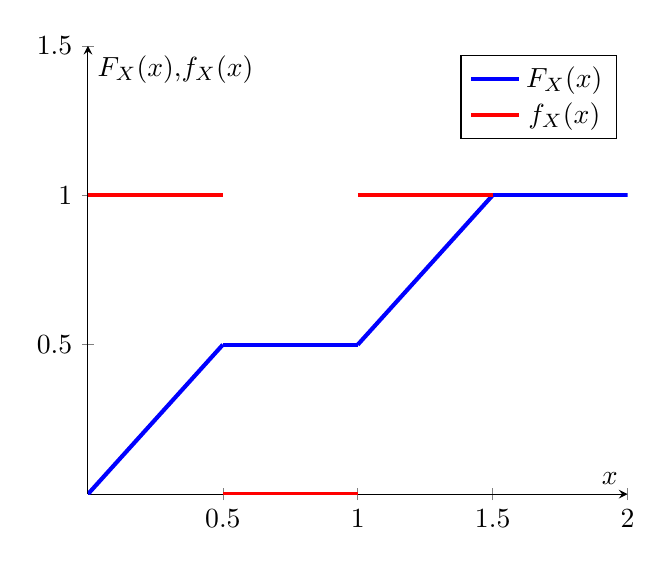
\begin{tikzpicture}
	\begin{axis}[
		axis lines = center,
		xlabel=$x$,
		ylabel={$F_X(x)$,$f_X(x)$},
		ymax=1.5,
		xtick={0,0.5,1,1.5,2}
	],
	\addplot[
		domain = 0:0.5,
		samples = 10,
		color = blue,
		line width = 1.5pt
	]{(x<0.5) * x};
	\addlegendentry{$F_X(x)$}
	\addplot[
		domain = 0:0.5,
		samples = 10,
		color = red,
		line width = 1.5pt
	]{(x<0.5) * 1};
	\addlegendentry{$f_X(x)$}
	\addplot[
		domain = 0.5:1,
		samples = 10,
		color = blue,
		line width = 1.5pt
	]{((x>=0.5) && (x<1)) * 0.5};
	\addplot[
		domain = 1:1.5,
		samples = 10,
		color = blue,
		line width = 1.5pt
	]{((x>=1) && (x<1.5)) * x - 0.5};
	\addplot[
		domain = 1.5:2,
		samples = 10,
		color = blue,
		line width = 1.5pt
	]{(x>=1.5) * 1};		
	\addplot[
		domain = 0.5:1,
		samples = 10,
		color = red,
		line width = 1.5pt
	]{((x>=0.5) && (x<1)) * 0};
	\addplot[
		domain = 1:1.5,
		samples = 10,
		color = red,
		line width = 1.5pt
	]{(x>=1) * 1};
	\end{axis}
\end{tikzpicture}
\end{center}
Ogni punto in $(\frac{1}{2},1)$ è \emph{mediana}, inoltre per ogni $X$
\emph{assolutamente continua} esiste una \emph{mediana}, ma non è detto che
sia unica. Lo è, solo se $F_X$ è invertibile in $m_X$.

\begin{observation}
	Se $X$ è una \emph{variabile aleatoria discreta}, la \emph{mediana} può non
	essere unica, ma non è detto che esista.
\end{observation}

\paragraph*{Esempio}
Sia \(X\sim bin(1,\frac{1}{2})\).
\begin{center}
\begin{tikzpicture}
	\begin{axis}[
		axis lines = center,
		xlabel=$x$,
		ylabel=$F_X(x)$,
		ymax=1.5,
		xmax=1.5
	]
	\addplot[
		domain = -0.5:0,
		samples = 10,
		color = blue,
		line width = 1.5pt
	]{(x<0) * 0};
	\addplot[
		domain = 0:1,
		samples = 10,
		color = blue,
		line width = 1.5pt
	]{((x>=0) && (x<1)) * 0.5};
	\addplot[
		domain = 1:1.5,
		samples = 10,
		color = blue,
		line width = 1.5pt
	]{(x>=1) * 1};
	\end{axis}
\end{tikzpicture}
\end{center}
Ogni punto in $(0,1)$ è \emph{mediana}.

\paragraph*{Esempio}
Sia $X$ una \emph{variabile aleatoria discreta} così definita:
\[X=\begin{cases}
	{0} & \text{con probabilità}\ {\frac{1}{6}}\\
	{2} & \text{con probabilità}\ {\frac{1}{1}}\\
	{2} & \text{con probabilità}\ {\frac{1}{3}}
\end{cases}\]
\begin{center}
\begin{tikzpicture}
	\begin{axis}[
		axis lines = center,
		xlabel=$x$,
		ylabel={$F_X(x)$, $\varphi_X(x)$},
		ymax=1.2,
		xmax=2.5,
		ymin=0,
		xmin=0,
		ytick={0,0.17,0.33,0.5,0.67,1},
		xtick={0,1,2},
		extra x ticks={0}
	]
	\addplot[
		domain = 0:1,
		samples = 100,
		color = blue,
		line width = 1.5pt
	]{(x<1) * 1/6};
	\addplot[
		domain = 1:2,
		samples = 10,
		color = blue,
		line width = 1.5pt
	]{((x>=1) && (x<2)) * (1/2+1/6)};
	\addplot[
		domain = 2:2.5,
		samples = 10,
		color = blue,
		line width = 1.5pt
	]{(x>=2) * 1};
	\node[circle,fill,inner sep=1.5pt] at (axis cs:0,0) {};
	\node[circle,fill,inner sep=1.5pt] at (axis cs:0,1/6) {};
	\node[circle,fill,inner sep=1.5pt] at (axis cs:1,0.5) {};
	\node[circle,fill,inner sep=1.5pt] at (axis cs:2, 1/3) {};
	\end{axis}
\end{tikzpicture}
\end{center}

In questo caso abbiamo:
\[x\in(-\infty, 1)\ P(X\leq x)\leq P(X=0)=\frac{1}{6} \Rightarrow P(X\geq x)\geq
P(X=1,X=2)=\frac{5}{6}\]
cioè tutti i valori per \(x\in(-\infty,1)\) sono sbilanciati verso sinistra e
quindi non posso essere una \emph{mediana}.
\[x\in(1,+\infty)\ P(X\leq x)\geq P(X\leq 1)=\frac{1}{2}+\frac{1}{6}=\frac{2}{3}
\Rightarrow P(X\geq x)\leq P(X=2)=\frac{1}{3}\]
Qui invece abbiamo il problema opposto in quanto i valori sono troppo sbilanciati
verso destra. L'ultima possibilità per avere una \emph{mediana} è che le condizioni
necessarie vengano soddisfatte per $x=1$.
\[x=1\ P(X\leq x)=\frac{2}{3}\neq\frac{5}{6}=P(X\geq 1)\]

Dunque, in questo caso, possiamo vedere come non esista alcun punto
\(m_X\in(-\infty,+\infty)\) tale che \(P(X\leq m_X)=P(X\geq m_X)\).

\begin{definition}
	Chiamiamo \emph{mediana impropria} un numero reale $\tilde{m}_X$ tale che:
	\[P(X\leq\tilde{m}_X)\geq\frac{1}{2}\wedge P(X\geq\tilde{m}_X\geq\frac{1}{2})\]
\end{definition}
\begin{observation}
	Nell'esempio sopra $x=1$ è una \emph{mediana impropria}.
\end{observation}

\subsection{Quantile}
\begin{definition}
	Data una \emph{variabile aleatoria} $X$ con legge $F_X$ e $p\in(0,1)$, chiamiamo
	\emph{p-quantile} (\emph{quantile p-esimo}, \emph{quantile p}) il numero reale:
	\[Q_X(p)=inf\{x\in\R:F_X(x)\geq p\}\]
\end{definition}

\begin{observation}
	La funzione \emph{quantile} \(Q_X:p\mapsto Q_X(p)\) con \(p\in(0,1)\) e \(Q_X(p)
	\in\R\), è qualcosa di simile all'inversa di $F_X$.
\end{observation}

\paragraph*{Esempio}
\texttt{qpois(p, lambda, lower.tail=TRUE)}
\begin{itemize}
	\item Se $p=\frac{k}{4}$ con \(k=1,2,3\) parliamo di \emph{quartili}
	\item Se $p=\frac{k}{10}$ con \(k=1,...,9\) parliamo di \emph{decili}
	\item Se $p=\frac{k}{100}$ con \(k=1,...,100\) parliamo di \emph{percentili}
\end{itemize}

\subsection{Moda}
\begin{definition}
	Chiamiamo \emph{moda} di una \emph{variabile aleatoria} $X$ il un numero
	$x\in\supp_X$ tale che:
	\begin{itemize}
		\item Se $X$ è \emph{discreta} $\varphi_X$ è massima in $x$, cioè \(x\in
		argmax_y\varphi_X(y)\)
		\item Se $X$ è \emph{assolutamente continua} $f_X$ è massima in $x$, cioè
		\(x\in argmax_y f_X(y)\)
	\end{itemize}
\end{definition}

\begin{observation}
	Intuitivamente possiamo pensare alla moda come ai valori più probabili.
	Proprio perché non è necessariamente unica distinguiamo tra \emph{variabili
	aleatorie unimodali} se hanno un'unica \emph{moda}, \emph{bimodali} se ne
	hanno 2 e \emph{multimodali} se ne hanno molte.
\end{observation}

\chapter{Modelli di variabili aleatorie assolutamente continue}

\section{Uniformi}
\begin{definition}
	Dati due numeri $a,b\in\R$ con $a<b$, chiamiamo una \emph{variabile aleatoria}
	$X$ \emph{uniforme} su $[a,b]$ se la sua \emph{densità} $f_X$ è costante in
	$[a,b]$ e nulla altrove. Scriveremo \(X\sim unif(a,b)\) oppure \(X\sim unif[a,b]\).
	\[1=\int_{-\infty}^{+\infty}f_Xdx=\int_a^bc\cdot dx=[c\cdot x]_a^b=c\cdot (b-a)\Rightarrow c=\frac{1}{b-a}\]
	\[f_X(x)=\begin{cases}
		{\frac{1}{b-a}} & \text{se}\ x\in(a,b)\\
		{0} & \text{altrimenti}
	\end{cases}\]
	\[F_X(x)=\begin{cases}
		{0} & \text{se}\ {x\leq a}\\
		{\int_{-\infty}^{+\infty}\frac{1}{b-a}dt=\int_a^x\frac{1}{b-a}dt} & 
			\text{se}\ {a<x\leq b}\\
		{1} & \text{se}\ {x>b}
	\end{cases}\Rightarrow\begin{cases}
		{0} & \text{se}\ {x\leq a}\\
		{\frac{x-a}{b-a}} & \text{se}\ {a<x\leq b}\\
		{1} & \text{se}\ {x>b}
	\end{cases}\]
\end{definition}

\begin{observation}
	Data $X\sim unif(a,b)$ gli indicatori visti finora assumono i seguenti valori:
	\begin{itemize}
		\item \(E[X]=\int_a^bx\cdot f_X(x)dx=\frac{1}{b-a}\cdot \int_a^bxdx=\frac{1}{b-a}\cdot \left[
			\frac{x^2}{2}\right]_a^b=\frac{1}{b-a}\cdot \frac{b^2-a^2}{2}=\frac{b+a}{2}\)
		\item \(Var[X]=\int_a^bx^2\cdot f_X(x)dx-\left(\frac{a+b}{2}\right)^2=\frac{1}{b-a}\cdot 
		\left[\frac{x^3}{3}\right]_a^b-\frac{(a+b)^2}{4}\left[\frac{x^2}{2}\right]_a^b
		=\frac{b^3-a^3}{3\cdot (b-a)}- \frac{(a+b)^2}{2}=\frac{(b-a)^2}{12}\)
		\item \(m_X=E[X]\) cioè la \emph{mediana} coincide con la \emph{media}
		\item \emph{Moda} qualunque valore in $(a,b)$
	\end{itemize}
\end{observation}
\subsection{Uniformi in R}
La famiglia di funzioni si chiama \texttt{unif}:
\begin{itemize}
	\item \texttt{dunif(x, min = 0, max = 1)}
	\item \texttt{punif(q, min = 0, max = 1, lower.tail = TRUE)}
	\item \texttt{runif(n, min = 0, max = 1)}
	\item \texttt{qunif(p, min = 0, max = 1, lower.tail = TRUE)}
\end{itemize}

\paragraph*{Esempio}
Un autobus passa ogni 15 minuti. Possiamo descrivere il tempo di attesa come
$X\sim unif(0,15)$. \(P(X<15)\)? \(P(X>10|X>5)\)?
\[P(X>5)=1-F_X(5)=1-\frac{5-0}{15-0}=1-\frac{5}{15}=1-\frac{1}{3}=\frac{2}{3}\]
\[P(X>10|X>5)=\frac{P(X>10, X>5)}{P(X>5)}=\frac{P(X>10)}{\frac{2}{3}}=\frac{1-
F_X(10)}{\frac{2}{3}}=\frac{1-\frac{10}{15}}{\frac{2}{3}}=\frac{\frac{1}{3}}
{\frac{2}{3}}=\frac{1}{2}\]

\section{Esponenziali}
\begin{definition}
	Una \emph{variabile aleatoria} $X$ è detta \emph{esponenziale}, di parametro
	\(\lambda\in\R\) con \(\lambda>0\), se:
	\[f_X(x)=\begin{cases}
		{0} & \text{se}\ {x<0}\\
		{c\cdot e^{-\lambda x}} & \text{se}\ {x\geq 0}
	\end{cases}\]
	In questo caso indicheremo in simboli \(X\sim exp(\lambda)\) o
	\(X\sim expo(\lambda)\). $\lambda$ viene detto anche \emph{rate} o \emph{intensità}.
\end{definition}

Non è difficile dimostrare che \(c=\lambda\). La \emph{funzione di ripartizione}
di una \emph{variabile aleatoria esponenziale} è:
\[F_X(x)=\begin{cases}
	{0} & \text{se}\ {x<0}\\
	{\int_0^x\lambda\cdot e^{-\lambda t}dt=\left[-e^{-\lambda t}\right]_0^x=1-e^{-\lambda x}} &
	\text{se}\ {x\geq 0}
\end{cases}\]

\begin{center}
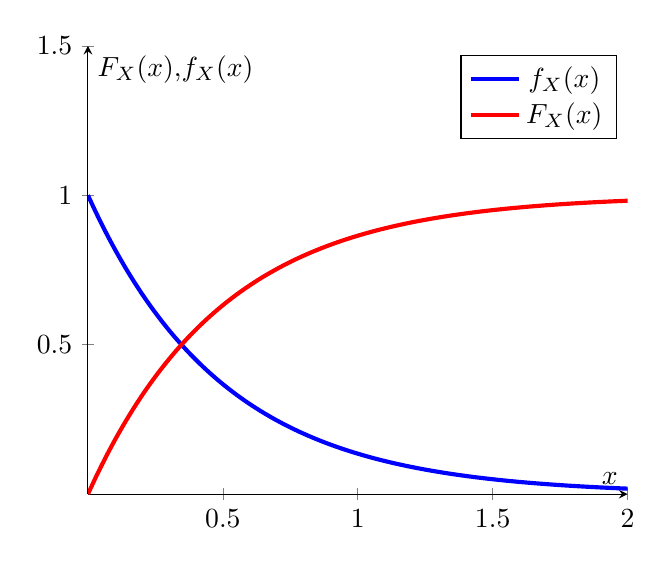
\begin{tikzpicture}
	\begin{axis}[
		axis lines = center,
		xlabel=$x$,
		ylabel={$F_X(x)$,$f_X(x)$},
		ymax=1.5
	],
	\addplot[
		domain = 0:2,
		samples = 200,
		color = blue,
		line width = 1.5pt
	]{e^(-2 * x)};
	\addlegendentry{$f_X(x)$}
	\addplot[
		domain = 0:2,
		samples = 200,
		color = red,
		line width = 1.5pt
	]{1-e^(-2 * x)};
	\addlegendentry{$F_X(x)$}
	\end{axis}
\end{tikzpicture}
\end{center}

\begin{observation}
	Data \(X\sim exp(\lambda)\) gli indicatori visti finora assumono i seguenti
	valori:
	\begin{itemize}
		\item \(E[X]=\int_0^{+\infty}x\cdot \lambda\cdot e^{-\lambda x}dx=\lambda\cdot \left[
		e^{-\lambda x}\cdot \frac{1}{\lambda^2}\cdot (\lambda x-1)\right]_0^{+\infty}=
		\frac{1}{\lambda}\)
		\item \(Var[X]=\int_0^{+\infty}x^2\cdot \lambda\cdot e^{-\lambda x}dx-\frac{1}
		{\lambda^2}=\frac{1}{\lambda^2}\)
		\item Vogliamo \(F_X(m_X)=\frac{1}{2}\Rightarrow 1-e^{-\lambda x}=\frac{1}{2}
		\Rightarrow e^{-\lambda x}=\frac{1}{2}\Rightarrow -\lambda\cdot x=\ln\left(
		\frac{1}{2}\right)\Rightarrow x=-\frac{\ln\left(\frac{1}{2}\right)}{\lambda}
		=\frac{\ln(2)}{\lambda}\Rightarrow m_X=\frac{\ln(2)}{\lambda}\)
		\item \emph{Moda} è 0 perché è il punto di massimo di $f_X$
	\end{itemize}
\end{observation}

\subsection{Esponenziali in R}
La famiglia di funzioni si chiama \texttt{exp}:
\begin{itemize}
	\item \texttt{dexp(x, rate = 1)}
	\item \texttt{pexp(q, rate = 1, lower.tail = TRUE)}
	\item \texttt{rexp(n, rate = 1)}
	\item \texttt{qexp(p, rate = 1, lower.tail = TRUE)}
\end{itemize}

\paragraph*{Esempio}
A una fermata dell'autobus il tempo medio di attesa è $\frac{15}{2}$. Supponiamo
di poter descrivere il tempo d'attesa come \(X\sim exp(\lambda)\). \(P(X<5)\)?
\(P(X>10|X>5)\)?

Sapendo la \emph{media}, possiamo ricavare facilmente il valore del parametro
$\lambda$, come \(\lambda=\frac{1}{E[X]}=\frac{2}{15}\).
\[P(X>5)=1-F_X(5)=1-(1-e^{-\lambda x})=e^{-\lambda x}=e^{-\frac{15}{2}\cdot 5}=e^{-
\frac{2}{3}}\approx 0.51\]
\[P(X>10|X>5)=\frac{P(X>10,X>5)}{P(X>5)}=\frac{1-F_X(10)}{1-F_X(5)}=e^{-\frac{20}{15}}
\cdot e^{\frac{2}{3}}=e^{-\frac{2}{3}}\approx 0.51\]

\begin{observation}
	Sapere di avere già aspettato 5 minuti, non ci dice nulla riguardo al futuro.
	Ciò ci suggerisce che probabilmente le \emph{variabili aleatorie esponenziali}
	non hanno memoria.
\end{observation}
\begin{proposition}
	Sia \(X\sim exp(\lambda)\). $X$ ha assenza di memoria, cioè presi \(t,s>0\),
	vale:
	\[P(X>s+t|X>s)=P(X>t)\]
\end{proposition}
\begin{demonstration}
	\[P(X>s+t|X>s)=\frac{P(X>s+t,X>s)}{P(X>s)}=\frac{1-F_X(s+t)}{1-F_X(s)}\]
	\[=\frac{e^{-\lambda(s+t)}}{e^{-\lambda(s)}}=e^{-\lambda t}=1-F_X(t)=P(X>t)\]	
\end{demonstration}

\begin{note}
	Le \emph{esponenziali} sono l'equivalente \emph{continuo} delle \emph{geometriche}.
\end{note}

\section{Gaussiane o normali}
\begin{definition}
	Una \emph{variabile aleatoria} $X$ è una \emph{normale standard} o se ha
	\emph{densità}:
	\[f_X(x)=\frac{1}{\sqrt{2\pi}}\cdot e^{-\frac{x^2}{2}}\]
	Scriveremo in simboli: \(X\sim\norm(0,1)\).
\end{definition}
\begin{observation}
	Possiamo notare le seguenti:
	\begin{itemize}
		\item \(e^{-\frac{x^2}{2}}\) da una forma a campana
		\item Il fattore $\frac{1}{2}$ a esponente è presente solo per comodità
		\item $\frac{1}{\sqrt{2\pi}}$ è la \emph{costante di rinormalizzazione}
	\end{itemize}
\end{observation}

\begin{property}
	La \emph{funzione di densità} di una \emph{normale standard} gode delle seguenti:
	\begin{enumerate}[label=(\roman*)]
		\item \emph{Simmetria assiale}: è simmetrica rispetto all'asse $x=0$
		\(\Rightarrow f_X(-x)=f_X(x)\)
		\item Ha il punto di massimo in $x=0$ e vale \(f_X(0)=\frac{1}{\sqrt{2\pi}}
		\approx0.4\)
		\item Ha dei punti di flesso in $x=\pm 1$ e in quei punti vale \(f_X(1)=
		f_X(-1)\approx0.24\)
		\item \(f_x(2)=f_X(-2)\approx0.05\)
		\item \(f_x(3)=f_X(-3)\approx0.004\)
	\end{enumerate}
\end{property}

\begin{observation}
	La \emph{funzione di ripartizione} di una \emph{normale standard} è la seguente:
	\[F_X(x)=\int_{-\infty}^x \frac{1}{\sqrt{2\pi}}\cdot e^{-\frac{-t^2}{2}}dt=\Phi(x)\]
\end{observation}

\begin{property}
	La \emph{funzione di ripartizione} gode delle seguenti:
	\begin{enumerate}[label=(\roman*)]
		\item \(F_X(0)=\Phi(0)=\frac{1}{2}\)
		\item \emph{Simmetria centrale}: è simmetrica rispetto a \((0,\frac{1}{2})\),
		quindi \(\Phi(-x)=1-\Phi(x)\)
		\item \(\Phi(-3)\approx0.0013\), \(\Phi(3)=1-\Phi(-3)\approx0.9987\)
		\item \(\Phi(-3)\approx0.0228\), \(\Phi(3)=1-\Phi(-3)\approx0.9772\)
		\item \emph{Monotonia}: è \emph{monotona strettamente crescente}, quindi
		è \emph{invertibile}
	\end{enumerate}
\end{property}

\begin{observation}
	Essendo $\Phi$ \emph{invertibile}, possiamo definire $\Phi^{-1}$ come la
	\emph{funzione quantile}:
	\[\Phi^{-1}(p)=x\Leftrightarrow F_X(x)=p\Leftrightarrow P(X\leq x)=p\]
	\(\Phi^{-1}:[0,1]\to\R\) è simmetrica rispetto al punto $(0,\frac{1}{2})$, cioè
	\(\Phi^{-1}(p)=-\Phi^{-1}(1-p)\).
\end{observation}

\begin{observation}
	Data $X\sim\norm(0,1)$ \emph{media} e \emph{varianza} assumono i seguenti valori:
	\begin{itemize}
		\item \(E[X]=\int_{-\infty}^{+\infty}x\cdot f_X(x)dx=\int_{-\infty}^{+\infty}
		x\cdot \frac{1}{\sqrt{2\pi}}\cdot e^{-\frac{x^2}{2}}dx=\int_{-\infty}^0x\cdot \frac{1}
		{\sqrt{2\pi}}\cdot e^{-\frac{x^2}{2}}dx+\int_0^{+\infty}x\cdot \frac{1}{\sqrt{2\pi}}
		\cdot e^{-\frac{x^2}{2}}dx\underrel{\xi=-x}{=}\int_{-\infty}^0 -\xi\cdot \frac{1}
		{\sqrt{2\pi}}\cdot e^{-\frac{x^2}{2}}dx+\int_0^{+\infty}x\cdot \frac{1}{\sqrt{2\pi}}
		\cdot e^{-\frac{x^2}{2}}=0\)
		\begin{note}
			Saremmo potuti giungere allo stesso risultato sfruttando il fatto che
			$x\cdot f_X(x)$ è una funzione \emph{dispari} e quindi simmetrica rispetto
			all'origine degli assi.
		\end{note}
		\item \(Var[X]=\int_{-\infty}^{+\infty}x^2\cdot \frac{1}{\sqrt{2\pi}}\cdot e^{-
		\frac{x^2}{2}}dx=\left[-x\cdot \frac{1}{\sqrt{2\pi}}\cdot e^{-\frac{x^2}{2}}\right]
		_{-\infty}^{+\infty}+\int_{-\infty}^{+\infty}\frac{1}{\sqrt{2\pi}}\cdot 
		e^{-\frac{x^2}{2}}=1\)
	\end{itemize}
\end{observation}

\begin{definition}
	Sia $Z\sim\norm(0,1)$. $X$ è una \emph{normale} o \emph{Gaussiana} di
	parametri $\mu,\sigma\in\R$ con $\sigma>0$ se:
	\[X=\sigma\cdot Z+\mu\]
	Scriveremo in simboli \(X\sim\norm(\mu, \sigma)\).
\end{definition}

\begin{observation}
	Dalle osservazioni fatte nel caso delle \emph{normali standard}, possiamo
	affermare che:
	\[F_X(x)=P(X\leq x)=P(\sigma\cdot Z+\mu\leq x)=P\left(Z\leq\frac{x-\mu}{\sigma}
	\right)=\Phi\left(\frac{x-\mu}{\sigma}\right)\]
	\[f_X(x)=\frac{1}{\sigma}\cdot \frac{1}{\sqrt{2\pi}}\cdot e^{-\frac{(x-\mu)^2}{2\sigma^2}}
	=\frac{1}{\sqrt{2\pi\sigma^2}}\cdot e^{-\frac{(x-\mu)^2}{2\sigma^2}}\]
\end{observation}

\begin{observation}
	Partendo dalle informazioni sulle \emph{normali standard} possiamo ricavare
	i valori della \emph{media} e della \emph{varianza} nel caso delle \emph{Gaussiane}.
	
	Siano $Z\sim\norm(0,1)$ e $X=\sigma\cdot Z+\mu$, con $\mu\in\R,\sigma>0$:
	\[E[X]=E[\sigma\cdot Z+\mu]=\sigma\cdot E[Z]+\mu=\mu\]
	\[Var[X]=Var[\sigma^2\cdot Z+\mu]=\sigma^2\cdot Var[Z]=\sigma^2\]
\end{observation}

\begin{proposition}
	Siano $X\sim\norm(\mu,\sigma)$ e $Z\sim\norm(0,1)$. $X$ eredita tutte le
	proprietà di $Z$ tenendo conto di dilatazione e traslazione.
\end{proposition}
\begin{proposition}
	La famiglia delle \emph{Gaussiane} è \emph{riproducibile}, cioè prese
	$X_1\sim\norm(\mu_1,\sigma_1)$ e $X_2\sim\norm(\mu_2,\sigma_2)$, vale:
	\[X_1+X_2\sim\norm(\mu_1+\mu_2, \sqrt{\sigma_1^2+\sigma_2^2})\]
\end{proposition}

\subsection{Normali in R}
La famiglia di funzioni si chiama \texttt{norm}:
\begin{itemize}
	\item \texttt{dnorm(x, mean = 0, sd = 1)}
	\item \texttt{pnorm(q, mean = 0, sd = 1, lower.tail = TRUE)}
	\item \texttt{qnorm(p, mean = 0, sd = 1, lower.tail = TRUE)}
	\item \texttt{rnorm(n, mean = 0, sd = 1)}
\end{itemize}

\section{Chi quadro}

\begin{definition}
	Se $X$ è la \emph{variabile aleatoria} definita come somma di quadrati di $n$
	\emph{normali standard} indipendenti, diciamo che $X$ è una \emph{Chi quadro}
	con $n$ \emph{gradi di libertà} (\emph{df}) e scriviamo \(X\sim\chi_n^2 \)
	oppure \(X\sim\chi^2(n)\).
	\[\{Y_i\}_{i=1}^n\ Y_i\sim\norm(0,1)\ X=\sum_{i=1}^nY^2_i\]
\end{definition}
\begin{observation}
	Se sommiamo due quadrati otteniamo un'\emph{esponenziale} di parametro
	\(\lambda=\frac{1}{2}\). La \emph{funzione di densità} è quindi definita in
	questo modo:
	\[f_X(x)=c_n\cdot x^{\frac{x}{2}}\cdot e^{-\frac{x}{2}}\ \text{con $c_n$ opportuna
	\emph{costante di rinormalizzazione}}\]
\end{observation}

Una volta definita la \emph{funzione di densità} può essere utile esaminare come
ne cambi la curva al variare dei \emph{gradi di libertà}.
\begin{center}
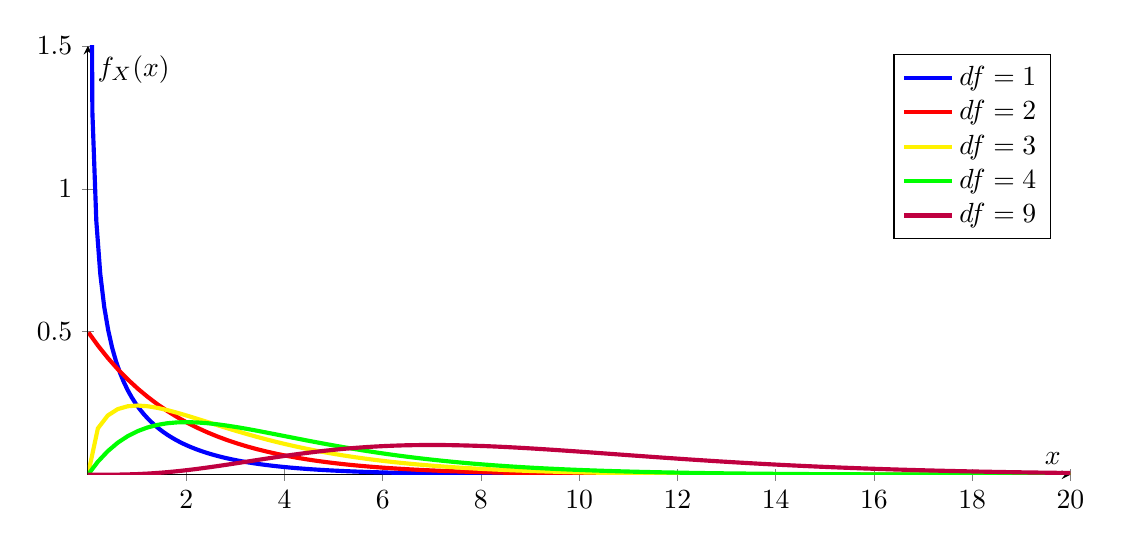
\begin{tikzpicture}
	\begin{axis}[
		axis lines = center,
		xlabel=$x$,
		ylabel={$f_X(x)$},
		ymax=1.5,
		xmax=20,
		width=400,
		height=200
	],
	\addplot[
		domain = 0.01:20,
		samples = 250,
		color = blue,
		line width = 1.5pt
	]{((x > 0) && (x <= 20)) * (0.398942 * x^(1/2 - 1) * e^(-x/2))};
	\addlegendentry{$df=1$}
	\addplot[
		domain = 0.01:20,
		samples = 100,
		color = red,
		line width = 1.5pt
	]{((x > 0) && (x <= 20)) * (0.5 * x^(2/2 - 1) * e^(-x/2))};
	\addlegendentry{$df=2$}
	\addplot[
		domain = 0:20,
		samples = 100,
		color = yellow,
		line width = 1.5pt
	]{((x > 0) && (x <= 20)) * (0.398942 * x^(3/2 - 1) * e^(-x/2))};
	\addlegendentry{$df=3$}
	\addplot[
		domain = 0:20,
		samples = 100,
		color = green,
		line width = 1.5pt
	]{((x > 0) && (x <= 20)) * (0.25 * x^(4/2 - 1) * e^(-x/2))};
	\addlegendentry{$df=4$}
	\addplot[
		domain = 0:20,
		samples = 100,
		color = purple,
		line width = 1.5pt
	]{((x > 0) && (x <= 20)) * (0.00379945 * x^(9/2 - 1) * e^(-x/2))};
	\addlegendentry{$df=9$}

	\end{axis}
\end{tikzpicture}
\end{center}

\begin{observation}
	Le \emph{Chi quadro} sono riproducibili per definizione. Quindi, se \(X\sim
	\chi_2(n)\) e \(Y\sim\chi_2(m)\), vale:
	\[X+Y\sim\chi_2(n+m)\]
\end{observation}

\begin{observation}
	Se \(X\sim\chi^2(n)\) \(X=\sum_{i=1}^nY^2_i\) con \(Y_i\sim\norm(0,1)\), vale:
	\[E[X]=E\left[\sum_{i=1}^nY_i\right]\underrel{\text{indipendenza}}{=}
	\sum_{i=1}^nE\left[Y^2_i\right]=n\]
	\[Var[X]=\sum_{i=1}^nVar[Y_i]=\sum_{i=1}^nE\left[Y^4_i\right]-\left(E\left[
	Y_i^2\right]\right)^2=\sum_{i=1}^n2=2n\]
\end{observation}

\subsection{Chi quadro in R}
La famiglia di funzioni si chiama \texttt{chisq}:
\begin{itemize}
	\item \texttt{dchisq(x, df)}
	\item \texttt{pchisq(q, df, lower.tail = TRUE)}
	\item \texttt{qchisq(p, df, lower.tail = TRUE)}
	\item \texttt{rchisq(n, df)}
\end{itemize}

\section{Distribuzione t di Student}

\begin{definition}
	Siano $Z\sim\norm(0,1)$ e $W\sim\chi^2(n)$ con $Z$ e $W$ indipendenti. $X$ è
	una \emph{t} di \emph{Student} a $n$ \emph{gradi di libertà} se:
	\[X=\frac{Z}{\sqrt{\frac{W}{n}}}\]
	Scriveremo in simboli \(X\sim t(n)\) oppure \(X\sim t_n\).
\end{definition}

\begin{note}
	Il grafico di una \emph{t} di \emph{Student} è simile al grafico di una
	\emph{normale}, con la differenza che la curva tende a stringersi e alzarsi
	all'origine all'aumentare dei \emph{gradi di libertà}.
\end{note}

\begin{property}
	Data $X\sim t(n)$, $X$ gode delle seguenti proprietà:
	\begin{enumerate}[label=(\roman*)]
		\item \emph{Densità}: \(f_X(-x)=f_X(x)\)
		\item \emph{Ripartizione}: \(F_X(-x)=1-F_X(x)\) con simmetria in $(0,\frac{1}{2})$
		\item \emph{Quantile}: \(F_X^{-1}(p)=-F_X^{-1}(1-p)\) con simmetria in
		$(\frac{1}{2},0)$
	\end{enumerate}
\end{property}

\begin{observation}
	Se $X\sim t(n)$, vale:
	\[E[X]=0\ \forall n\]
	\[Var[X]=\begin{cases}
		{\text{indefinita}} & \text{se}\ {n=1}\\
		{+\infty} & \text{se}\ {n=2}\\
		{\frac{n}{n-2}} & \text{se}\ {n>2}
	\end{cases}\]
\end{observation}

\begin{note}
	La \emph{speranza} di una \emph{t} di \emph{Student} è $0$ perché la
	\emph{speranza} di una \emph{normale standard} è costantemente $0$.
\end{note}

\begin{observation}
	Si noti che se $X\sim t(n)$ \(\lim_{n\to +\infty}Var[X]=1\).
\end{observation}

\begin{observation}
	Se \(X\sim t(n)\), dalla definizione sappiamo che \(X=\frac{Z}{\sqrt{\frac{W}{n}}}\)
	con $Z\sim\norm(0,1)$ e $W\sim\chi^2(n)$. Proviamo a studiare il denominatore
	\(\frac{W}{n}\):
	\[E\left[\frac{W}{n}\right]=\frac{E[W]}{n}=\frac{n}{n}=1\]
	\[Var\left[\frac{W}{n}\right]=\frac{Var[W]}{n^2}=\frac{2n}{n^2}=\frac{2}{n}\]
	
	Si noti che \(\lim_{n\to +\infty}Var[\frac{W}{n}]=0\), quindi, in un certo
	senso, al crescere di $n$ le \emph{t} di \emph{Student} si distribuiscono
	come una \emph{normale standard}.
\end{observation}

\subsection{t di Student in R}
La famiglia di funzioni si chiama \texttt{t}:
\begin{itemize}
	\item \texttt{dt(x, df)}
	\item \texttt{pt(q, df, lower.tail = TRUE)}
	\item \texttt{qt(p, df, lower.tail = TRUE)}
	\item \texttt{rt(n, df)}
\end{itemize}

\chapter{Convergenza di variabili aleatorie}

\section{Tipi di convergenza}
\begin{definition}[Convergenza quasi certa]
	Sia $\probspace$ uno \emph{spazio di probabilità} e siano $X$ una
	\emph{variabile aleatoria} su di esso e \(\{X_n\}_{n\in\N}\) una successione
	di \emph{variabili aleatorie} sullo stesso spazio. Diciamo che \(\{X_n\}_{n\in\N}\)
	\emph{converge quasi certamente} o \emph{puntualmente} a $X$ se:
	\[\exists E\in\F\ \text{con}\ P(E)=1\ t.c.\ \forall\omega\in E\ \lim_{n\to
	+\infty}X_n(\omega)=X(\omega)\]
	Scriveremo in simboli:
	\[X_n\conv{q.c}{n}X\]
\end{definition}
\begin{definition}[Convergenza in probabilità]
	Siano \(\{X_n\}_{n\in\N}\) una successione di \emph{variabili aleatorie} e
	$X$ una \emph{variabile aleatoria} su $\probspace$. Diciamo che \(\{X_n\}_
	{n\in\N}\) \emph{converge in probabilità} se:
	\[\forall\epsilon>0\ \lim_{n\to +\infty}P(|X_n-X|>\epsilon)=0\]
	Scriveremo in simboli:
	\[X_n\conv{P}{n}X\]
\end{definition}
\begin{definition}[Convergenza in media quadratica]
	Siano \(\{X_n\}_{n\in\N}\) una successione di \emph{variabili aleatorie} e
	$X$ una \emph{variabile aleatoria} su $\probspace$. Diciamo che \(\{X_n\}_
	{n\in\N}\) \emph{converge in media quadratica} se:
	\[\lim_{n\to +\infty}E\left[|X_n-X|^2\right]=0\]
	Scriveremo in simboli:
	\[X_n\conv{L^2}{n}X\]
\end{definition}

\begin{proposition}
	La \emph{convergenza in media quadratica} implica la \emph{convergenza in
	probabilità}, cioè:
	\[X_n\conv{L^2}{n}X\Rightarrow X_n\conv{P}{n}X\]
\end{proposition}
\begin{demonstration}
	Fissiamo $\epsilon>0$:
	\[P(|X_n-X|>\epsilon)=P(|X_n-X|^2>\epsilon^2)\underrel{Markov}{\leq}
	\frac{E\left[|X_n-X|^2\right]}{\epsilon^2}\]
	A questo punto se prendiamo il limite per \(n\to +\infty\) otteniamo:
	\[\lim_{n\to +\infty}P(|X_n-X|>\epsilon)\leq\frac{\lim_{n\to +\infty}E\left[
	|X_n-X|^2\right]}{\epsilon^2}=0\]
	L'ultima uguaglianza è garantita dalla definizione di \emph{convergenza in
	media quadratica}.
\end{demonstration}

\begin{proposition}
	La \emph{convergenza quasi certa} implica la \emph{convergenza in probabilità},
	cioè:
	\[X_n\conv{q.c.}{n}X\Rightarrow X_n\conv{P}{n}X\]
\end{proposition}

\begin{observation}
	Dalle precedenti proposizioni otteniamo che:
	\[X_n\conv{L^2}{n}X\Rightarrow X_n\conv{P}{n}X\]
	\[X_n\conv{q.c.}{n}X\Rightarrow X_n\conv{P}{n}X\]
	Quindi, la \emph{convergenza in media quadratica} e la \emph{convergenza
	quasi certa} non sono confrontabili.
\end{observation}

\begin{definition}
	Siano \(\{X_n\}_{n\in\N}\) una successione di \emph{variabili aleatorie} su
	$\probspace$ e $X$ una \emph{variabile aleatoria} su \((\tilde{\Omega},\tilde{\F},
	\tilde{P})\). Diciamo che \(\{X_n\}_{n\in\N}\) \emph{converge in distribuzione},
	in \emph{legge} o \emph{debolmente} a $X$ se:
	\[\forall x\in\R\ \lim_{n\to +\infty}P(X_n\leq x)=P(X\leq x)\text{, ossia}\ 
	\lim_{n\to +\infty}P(X_n\leq x)=F_X(x)\]
	Scriveremo in simboli:
	\[X_n\conv{\mathcal{L}}{n}X, X_n\conv{d}{n}X\ \text{o}\ X_n\conv{\omega}
	{n}X\]
\end{definition}

\begin{proposition}
	La \emph{convergenza in probabilità} implica la \emph{convergenza debole},
	cioè:
	\[X_n\conv{P}{n}X\Rightarrow X_n\conv{d}{n}X\]
\end{proposition}
\begin{note}
	Per \emph{transitività} gli altri due tipi di convergenza implicano
	\emph{convergenza debole}, cioè:
	\[X_n\conv{L^2}{n}X\Rightarrow X_n\conv{P}{n}X\Rightarrow X_n\conv{d}{n}X\]
	\[X_n\conv{q.c.}{n}X\Rightarrow X_n\conv{P}{n}X\Rightarrow X_n\conv{d}{n}X\]
\end{note}

\section{Teoremi limite}
\begin{proposition}
	Sia \((X_1,X_2,\dots,X_n)\) un \emph{vettore aleatorio} con componenti
	indipendenti tra loro, di \emph{media} e \emph{varianza} comuni $\mu$ e $\sigma^2$.
	Sia \(S_n=\sum_{i=1}^nX_i\) la \emph{variabile aleatoria} somma. Allora, vale:
	\[E\left[\frac{S_n}{n}\right]=\mu\]
	\[Var\left[\frac{S_n}{n}\right]=\frac{\sigma^2}{n}\]
\end{proposition}
\begin{demonstration}
	Per \emph{linearità} della \emph{speranza} otteniamo:
	\[Var\left[\frac{S_n}{n}\right]=\frac{1}{n^2}\cdot \sum_{i=1}^nVar[X_i]=\frac{1}
	{n^2}\cdot n\cdot \sigma^2=\frac{\sigma^2}{n}\]
\end{demonstration}

\begin{theorem}[Legge debole dei grandi numeri]
	Sia \(\{X_n\}_{n\in\N}\) una successione di \emph{variabili aleatorie} indipendenti,
	ciascuna di \emph{media} $\mu$	e \emph{variazione finita} $\sigma^2$. Sia
	inoltre \(S_n=\sum_{i=1}^nX_i\) la \emph{variabile aleatoria} somma. La
	\emph{variabile aleatoria} \(\frac{S_n}{n}\conv{P}{n}\mu\), cioè:
	\[\forall\epsilon>0\ \lim_{n\to +\infty}P(|S_n-\mu|>\epsilon)=0\]
\end{theorem}
\begin{demonstration}
	\[P\left(|\frac{S_n}{n}-\mu|>\epsilon\right)=P\left(|\frac{S_n}{n}-E\left[
	\frac{S_n}{n}\right]|>\epsilon\right)\underrel{Chebychev}{\leq}\frac{Var\left[
	\frac{S_n}{n}\right]}{\epsilon^2}=\frac{\sigma^2}{\epsilon^2}\cdot \frac{1}{n}\]
	A questo punto facendo il limite per \(n\to +\infty\) si ottiene:
	\[\lim_{n\to +\infty}\frac{\sigma^2}{\epsilon^2}\cdot \frac{1}{n}=0\]
\end{demonstration}

\paragraph*{Esempio}
Sia $p=\frac{1}{2}$. Consideriamo il \emph{processo di Bernoulli} di parametro
$p$: \(\{X_n\}_{n\in\N}\) con \(X_i\sim bin(1,\frac{1}{2})\) iid e quindi
\(S_n\sim bin(n, \frac{1}{2})\). La \emph{legge debole dei grandi numeri} ci dice
che \(\frac{S_n}{n}\conv{P}{n}\frac{1}{2}\).

Vogliamo confrontare $S_n$ con $\frac{1}{2}$
\[\frac{S_n}{n}\conv{P}{n}\frac{1}{2}\Rightarrow\frac{S_n}{n}-\frac{1}{2}\conv{P}
{n}0\Rightarrow\frac{S_n-\frac{n}{2}}{n}\conv{P}{n}0\]

\begin{theorem}[Teorema centrale del limite]
	Sia \(\{X_n\}_{n\in\N}\) una successione di \emph{variabili aleatorie}
	indipendenti di \emph{media} $\mu$ e \emph{varianza finita} $\sigma^2$. Se
	\(S_n=\sum_{i=1}^nX_i\) allora, vale:
	\[\frac{S_n-n\cdot \mu}{\sigma\cdot \sqrt{n}}\conv{d}{n}\norm(0,1)\text{, cioè}\ \lim_
	{n\to +\infty}P\left(\frac{S_n-n\cdot \mu}{\sigma\cdot \sqrt{n}}\leq x\right)=\Phi(x)\]
\end{theorem}

\begin{observation}
	Nella pratica, non si usa mai il \emph{teorema centrale dei grandi numeri} in
	quanto, non si lavora mai su infinite \emph{variabili aleatorie} $X_i$, ma
	su un numero finito. Quindi, useremo il teorema per avere delle approssimazioni
	nel caso $n$ sia sufficientemente grande. In qual caso otteniamo:
	\[\frac{S_n-n\cdot \mu}{\sigma\cdot \sqrt{n}}\dot{\sim}\norm(0,1)\Rightarrow \frac{S_n}
	{n}\dot{\sim}\norm(\mu, \frac{\sigma}{\sqrt{n}})\Rightarrow S_n\dot{\sim}\norm
	(n\cdot \mu, \sqrt{n}\cdot \sigma)\]
\end{observation}

\paragraph*{Esempio}
Un calcolatore somma $10^6$ numeri con un errore di arrotondamento in ogni operazione.
Gli errori sono distribuiti in modo uniforme sull'intervallo \([-0.5\cdot 10^{-10},
0.5\cdot 10^{-10}]\). Qual è la probabilità che l'errore totale sia minore di $0.5\cdot 10^{-7}$?

Sia $X_i\sim unif(-0.5\cdot 10^{-10}, 0.5\cdot 10^{-10})$ la \emph{variabile aleatoria} che
descrive l'errore di una singola somma. L'errore totale sarà \(S_n=\sum_{i=1}^n
X_i\) con $n=10^6$.

Cerchiamo \(P(|S_n|\leq0.5\cdot 10^{-7})=P(|S_n|<0.5\cdot 10^{-7})\).
In questo caso non ci interessa distinguere tra $<$ e $\leq$ in quanto stiamo
lavorando con \emph{variabili aleatorie assolutamente continue}.
\[P(|S_n|<0.5\cdot 10^{-7})=P(S_n<0.5\cdot 10^{-7})-P(S_n<-0.5\cdot 10^{-7})\]
Dal \emph{teorema centrale del limite} sappiamo che
\[\frac{S_n-n\cdot E[X_i]}{\sqrt{n}\cdot \sqrt{Var[X_i]}}\dot{\sim}\norm(0,1)\Leftrightarrow
P\left(\frac{S_n-n\cdot E[X_i]}{\sqrt{n}\cdot \sqrt{Var[X_i]}}\leq x\right)\simeq\Phi(x)\]
Ora, sarebbe comodo riscrivere il risultato ottenuto sopra in modo da arrivare a
una forma del tipo \(P(S_n\leq y)\):
\[P\left(S_n\leq \sqrt{n\cdot Var[X_i]}\cdot x+n\cdot E[X_i]\right)\simeq\Phi(x)\]
A questo punto ricaviamo $x$:
\[n\cdot Var[X_i]\cdot x+n\cdot E[X_i]=y\Leftrightarrow x=\frac{y-n\cdot E[X_i]}{\sqrt{n}\cdot 
\sqrt{Var[X_i]}}\]

Notiamo che saremmo potuti arrivare allo stesso risultato ricordando che \(S_n
\dot{\sim}\norm(y-n\cdot E[X_i], \sqrt{n}\cdot \sqrt{Var[X_i]})\), e di conseguenza,
sfruttando le proprietà delle \emph{Gaussiane}, arrivare ad avere:
\[P(S_n\leq x)=F_{S_n}(y)=\Phi\left(\frac{y-n\cdot E[X_i]}{\sqrt{n}\cdot \sqrt{Var[X_i]}}\right)\]
Ora non ci resta che svolgere i calcoli veri e proprio, inserendo nell'espressione,
i seguenti valori:
\begin{itemize}
	\item $n=10^6$
	\item $E[X_i]=0$
	\item $Var[X_i]=\frac{10^{-20}}{12}$
	\item $y=\pm 0.5\cdot 10^{-7}$
\end{itemize}
Quindi
\[P(S_n<0.5\cdot 10^{-7})=P(S_n<0.5\cdot 10^{-7})-P(S_n<-0.5\cdot 10^{-7})=\]
\[F_{S_n}(0.5\cdot 10^{-7})-F_{S_n}(-0.5\cdot 10^{-7})=F_{S_n}(0.5\cdot 10^{-7})-(1-F_{S_n}(0.5\cdot 10^{-7}))\]
\[2\cdot F_{S_n}(0.5\cdot 10^{-7})-1\simeq2\cdot \Phi\left(\frac{0.5\cdot 10^{-7}}{10^3\cdot \frac{10^{-10}}
{\sqrt{12}}}\right)-1\simeq2\cdot \Phi(1.75)-1=1.9108-1\approx91\%\]
La probabilità che l'errore totale sia minore di $0.5\cdot 10^{-7}$ è circa $91\%$.

\begin{observation}
	Nell'esempio appena visto abbiamo trattato la relazione $<$ come quella $\leq$
	e viceversa. Lo abbiamo potuto fare perché stavamo lavorando con \emph{variabili
	aleatorie assolutamente continue}, ma, nel caso di \emph{variabili aleatorie
	discrete}, questo tipo di semplificazioni avrebbe potuto provocare errori.

	Per risolvere questo inconveniente si può fare affidamento sulla
	\emph{correzione di continuità}.
\end{observation}

\begin{observation}
	In precedenza ci siamo posti il problema di poter lavorare solo con un
	numero finito di \emph{variabili aleatorie} e di dover quindi ricorrere ad
	approssimazioni e che per ottenere un risultato vicino al valore reale c'è
	bisogno di una parametro $n$ che si sufficientemente grande. Ma quanto grande
	deve essere?

	La risposta dipende dal modello delle \emph{variabili aleatorie} che si stanno
	considerando:
	\begin{itemize}
		\item \emph{Normali} [$X_i\sim\norm$]: grazie alla \emph{riproducibilità}
		è sufficiente $n\geq 1$
		\item \emph{Uniformi} [$X_i\sim unif$]: $n\geq 5$
		\item \emph{Esponenziali} [$X_i\sim exp$]: $n\geq 15$
		\item \emph{Geometriche} [$X_i\sim geom$]: $n\geq 15$
		\item \emph{Chi quadro} [$X_i\sim\chi^2$]: $n\geq 25$.\\
		Possiamo però sfruttare la \emph{riproducibilità} \(X_i\sim\chi^2_n\dot
		{\sim}\norm(n,\sqrt{2n})\), quindi se sommiamo \(\chi^2(1)\) ne occorrono
		almeno $25$, ma se sommiamo \(\chi^2(9)\) ne bastano circa $3$
		\item \emph{Binomiali} [$X_i\sim bin$]: in questo caso è necessario che
		$p$ non sia troppo "sbilanciata", cioè che non sia troppo vicina ai
		valori limite $0$ e $1$. In tal caso possiamo sfruttare il \emph{teorema
		centrale del limite} per approssimare la distribuzione stessa:
		\[bin(n,p)\dot{\sim}\norm(n\cdot p, \sqrt{n\cdot p\cdot (1-p)})\]
		La condizione su $p$ dipende da $n$ e in generale si richiede che \(n\cdot p\cdot 
		(1-p)\apprge3\)
		\item \emph{Poissoniane} [$X_i\sim pois$]: sfruttiamo la \emph{riproducibilità}
		\[pois(\lambda)\dot{\sim}\norm(\lambda, \sqrt{\lambda})\]
		Ricordiamo infatti, che una \emph{Poissoniana} di parametro $\lambda$ può
		essere vista come la somma di $n$ \emph{Poissoniane} di parametro
		$\tilde{\lambda}=\frac{\lambda}{n}$. Per $\lambda\apprge30$ otteniamo
		una buona approssimazione.
	\end{itemize}
\end{observation}

\chapter{Statistica}

\section{Generalità sulla statistica}
\begin{definition}
	Si definisce \emph{popolazione di riferimento} l'insieme di elementi, distinti
	tra loro, sui quali viene condotta un'indagine. I singoli elementi vengono
	detti \emph{individui}, \emph{esemplari} o \emph{unità statistiche}.
\end{definition}

Riprendendo le definizioni di \emph{statistica descrittiva} e \emph{inferenziale},
possiamo esaminarne in modo più preciso le differenze. In entrambe vogliamo
studiare alcune caratteristiche di una popolazione, ma, mentre nella \emph{statistica
descrittiva} abbiamo dati sulla totalità della popolazione, la \emph{statistica
inferenziale}, ne considera invece solo un \emph{campione} e utilizza poi
metodi probabilistici per ricavare (o inferire) informazioni generalizzate.

\begin{definition}
	Un \emph{campione} è un sottoinsieme della popolazione.
\end{definition}

Il concetto di \emph{campione} è molto simile a quello di \emph{evento} in
probabilità.  Sia i \emph{campioni} che gli \emph{eventi} infatti, sono
rispettivamente, sottoinsiemi della \emph{popolazione} e dell'\emph{universo}.
È quindi logico pensare che ci siano delle regole da rispettare per scegliere
un \emph{campione} adatto, proprio come ce n'erano per la definizione di una
\emph{tribù}.

\begin{observation}
	Esistono diversi tipi di campionamento, tra cui:
	\begin{itemize}
		\item \emph{Campionamento casuale semplice}
		\item \emph{Campionamento stratificato}
		\item \emph{Campionamento a grappolo}
	\end{itemize}
\end{observation}

\begin{definition}
	Le caratteristiche che misuriamo prendono il nome di \emph{variabili} e i loro
	valori prendono il nome di \emph{modalità} o \emph{livelli}. Le \emph{variabili}
	possono essere di tipo:
	\begin{itemize}
		\item \emph{Qualitative o categoriche}: se sono grandezze non numeriche
		\begin{itemize}
			\item \emph{Nominali}: se non hanno un ordine naturale (e.g. colore dei capelli)
			\item \emph{Ordinali}: se hanno un ordine naturale (e.g. titolo di studio)
		\end{itemize}
		\item \emph{Quantitative o numeriche}: se sono grandezze numeriche
		\begin{itemize}
			\item \emph{Discrete}: se sono descritte da numeri interi (e.g. numero di persone)
			\item \emph{Continue}: se sono descritte da numeri reali (e.g. una misura di tempo o distanza)
		\end{itemize}
	\end{itemize}

	Nel caso di \emph{variabili numeriche}, la scala di misurazione può essere
	di due tipi:
	\begin{itemize}
		\item \emph{Intervallo}: se lo $0$ è scelto in modo arbitrario
		\item \emph{Rapporto}: se lo $0$ è fissato in modo naturale
	\end{itemize}
\end{definition}

\begin{definition}
	Una \emph{statistica} è una funzione calcolabile a partire dalla misurazione
	di un \emph{campione}.
\end{definition}

\paragraph{Esempio}
I seguenti sono esempi di \emph{statistiche} calcolabili su un campione
\((x_1,\dots,x_n)\):
\begin{itemize}
	\item \emph{Media campionaria}: \(\bar{x}\coloneqq\frac{1}{n}\cdot \sum_{i=1}^nx_i\)
	\item \emph{Varianza campionaria a media (o speranza) $\mu$ nota}: \(s_\cdot ^2
	\coloneqq\frac{1}{n}\cdot \sum_{i=1}^n(x_i-\mu)^2\)
	\item \emph{Varianza campionaria a media (o speranza) $\mu$ ignota}: \(s^2
	\coloneqq\frac{1}{n-1}\cdot \sum_{i=1}^n(x_i-\bar{x})^2\)
	\item Il numero di misurazione eccedenti una certa soglia \(c\coloneqq \#\{
	i\in\{1,\dots,n\}:x_i>c\}\)
	\item Il primo esemplare del campione la cui misurazione è inferiore a una
	certa soglia: \(c\coloneqq\inf\{i\in\{1,\dots,n\}:x_i<c\}\)
\end{itemize}

\begin{observation}
	Se gli $x_i$ sono indicati con la minuscola, stiamo parlando di quantità,
	valori numerici, se invece scriviamo $X_i$, indichiamo le \emph{variabili
	aleatorie} rappresentanti i singoli \emph{esemplari}. La stessa notazione è
	estesa alle \emph{funzioni statistiche}, ad esempio $s^2$ sarà un numero,
	mentre $S^2$ una \emph{variabile aleatoria} o il risultato di un
	\emph{esperimento aleatorio}.
\end{observation}

\paragraph{Esempio}
Una ditta produce bulloni con un diametro di $7mm$. Un bullone è accettabile se
ha un diametro compreso tra $6.5mm$ e $7.5mm$.  Preso un bullone ne misuriamo il
diametro effettivo. Il nostro obiettivo è usare queste misurazioni per risalire
a una funzione $f_X$ che possa essere usata per descrivere il diametro di tutti
i bulloni prodotti.

\paragraph{}
Ci sono molti modi in cui la funzione $f_X$ può essere ignota. Noi ci limiteremo
a considerare il caso in cui sia noto il tipo di distribuzione della \emph{variabile
aleatoria}, ma non ne conosciamo i parametri. Ad esempio, potremmo sapere che $X$
è una \emph{Poissoniana}, ma non conosciamo $\lambda$. Il nostro scopo è quindi
usare i dati a nostra disposizione per ricavare $\lambda$, o equivalentemente,
il \emph{valore atteso}.

\section{Stimatori e stime}
Si dice \emph{stimatore} di un parametro una \emph{variabile aleatoria} che sia
una \emph{statistica} e il cui valore sia "spesso vicino" al parametro che ci
interessa.

Il valore deterministico assunto dallo \emph{stimatore} usando i dati ricavati
prende il nome di \emph{stima}.

\begin{note}
	Si noti che lo \emph{stimatore} è una funzione definita sul campione che ha
	come parametri i dati delle osservazioni, mentre la \emph{stima} è un numero.
\end{note}

\paragraph{Esempio}
Sia \((X_1,\dots,X_n)\) un \emph{vettore di variabili aleatorie} indipendenti e
identicamente distribuite. Come parametro di interesse abbiamo \(E[X_i]=\mu\).

Uno \emph{stimatore} della \emph{media} può essere la \emph{media campionaria}
\(\hat{\mu}=\bar{X}=\frac{1}{n}\cdot \sum_{i=1}^nX_i\). $\bar{X}$ è uno \emph{stimatore}
per $\mu$, cioè $\bar{X}\approx\mu$, in quanto, per la \emph{legge dei grandi
numeri}, vale:
\[\frac{\sum_{i=1}^nX_i}{n}=\frac{1}{n}\cdot \sum_{i=1}^nX_i=\{\bar{X}\}_n\conv{P}{n}\mu\]
\newpage
\begin{note}
	Se $\Theta$ è uno \emph{stimatore} di $\vartheta$, possiamo scrivere $\Theta_n$
	per evidenziare la numerosità del campione. In particolare, vale che \(\Theta_n
	=\hat{\vartheta}(\{X_i\}_{i=1}^n)\).
\end{note}

\begin{observation}
	Essendo $\Theta$ una \emph{stima}, è ragionevole aspettarsi un qualche scostamento
	dal valore effettivo. Questo errore, detto \emph{errore di stima}, è anch'esso
	una \emph{variabile aleatoria}. Siccome nella definizione di \emph{stimatore}
	abbiamo chiesto che il valore stimato fosse vicino al parametro interessato,
	ci aspettiamo che l'errore sia piccolo.
\end{observation}

\begin{definition}
	Uno \emph{stimatore} $\Theta$ di $\vartheta$ è:
	\begin{itemize}
		\item \emph{Corretto, non distorto o unbiased} se $E[\Theta]=\vartheta$
		\item \emph{Scorretto o biased} se $E[\Theta]\neq\vartheta$ e chiamiamo
		\emph{bias} il valore $E[\Theta]-\vartheta$
	\end{itemize}
	In particolare, se \(\lim_{n\to +\infty}E[\Theta_n]=\vartheta\), allora $\Theta$
	è detto \emph{asintoticamente non distorto}.
\end{definition}

\begin{definition}
	Si dice \emph{errore quadratico medio} di $\Theta$, il valore:
	\[MSE[\Theta]=E\left[(\Theta-\vartheta)^2\right]\]  
\end{definition}

\begin{observation}
	L'\emph{errore quadratico medio} può essere riscritto in una maniera un po'
	diversa:
	\[MSE[\Theta]=E\left[(\Theta-\vartheta)^2\right]=E\left[(\Theta-E[\Theta]+
	E[\Theta]-\vartheta)^2\right]\]
	\[=E\left[(\Theta-E[\Theta])^2\right]+2E\left[(\Theta-E[\Theta])\cdot (E[\Theta]-
	\vartheta)\right]+E[(E[\Theta]-\vartheta)^2]\]
	\[=Var[\Theta]+2E\left[(E[\Theta]-E[\Theta])\cdot (\Theta-\vartheta)\right]+(bias)
	^2=Var[\Theta]+(bias)^2\]
	In particolare se $\Theta$ è \emph{corretto}, il \emph{bias} è nullo e quindi
	\(MSE[\Theta]=Var[\Theta]\).
\end{observation}

\begin{definition}
	Diciamo che uno \emph{stimatore} $\Theta$ è \emph{consistente}, se $\Theta_n$
	\emph{converge in probabilità} a $\vartheta$, cioè se vale:
	\[\Theta_n\conv{P}{n}\vartheta\]
	Se, inoltre, $\Theta_n$ \emph{converge in media quadratica} a $\vartheta$,
	ovvero se vale:
	\[\Theta_n\conv{L^2}{n}\vartheta\]
	diciamo che $\Theta$ è \emph{consistente in media quadratica}.
\end{definition}

\begin{proposition}
	Se $\Theta$ è \emph{asintoticamente non distorto} e \(\lim_{n\to+\infty}Var
	[\Theta]=0\), allora $\Theta$ è uno \emph{stimatore consistente in media
	quadratica} e quindi è anche \emph{consistente}.
\end{proposition}

\begin{demonstration}
	Chiedere che $\Theta$ sia \emph{consistente in media quadratica} significa
	chiedere che:
	\[\lim_{n\to+\infty}E\left[(\Theta_n-\vartheta)^2\right]=0\]
	ossia che \(\lim_{n\to+\infty}MSE[\Theta_n]=0\), ma per quanto visto nell'ultima
	osservazione
	\[MSE[\Theta_n]=Var[\Theta_n]+(E[\Theta_n]-\vartheta)^2\]
	e la convergenza a $0$ è assicurata dalle ipotesi applicate ai due addendi
	del secondo membro. La \emph{consistenza} segue dal fatto che siccome la
	\emph{convergenza in media quadratica} implica \emph{convergenza in probabilità},
	la \emph{consistenza in media quadratica} non può che implicare \emph{consistenza}.
\end{demonstration}

\begin{observation}
	Uno \emph{stimatore} può essere \emph{corretto}, ma non \emph{consistente}.
	Ad esempio, se \((X_1,\dots,X_n)\) è un \emph{vettore di variabili aleatorie}
	indipendenti e identicamente distribuite, ogni $X_i$ è uno \emph{stimatore}
	della \emph{media} $\mu$, poiché \(E[X_i]=\mu\ \forall i\in\{1,\dots,n\}\).
	Se prendiamo \(\sigma^2=Var[X_i]\neq 0\), allora \(P(|X_i-\mu|>\epsilon)\neq0\)
	e rimane tale per \(n\to+\infty\), quindi non vi è \emph{convergenza in
	probabilità}.
\end{observation}

\subsection{Alcuni stimatori}
Supponiamo di avere come \emph{campione} \((X_1,\dots,X_n)\), cioè un vettore di
\emph{variabili aleatorie iid} di \emph{media} \(E[X_i]=\mu\) e \emph{varianza}
\(Var[X_i]=\sigma^2\):
\begin{itemize}
	\item La \emph{media campionaria} \(\hat{\mu}=\hat{\mu_n}=\bar{X}=\bar{X_n}
	=\frac{1}{n}\cdot \sum_{i=1}^nX_i\) è uno \emph{stimatore corretto e consistente}
	della \emph{speranza}, ovvero \(E[X_i]=\mu\). Valgono infatti le seguenti:
	\[E[\hat{\mu}]=E\left[\frac{1}{n}\cdot \sum_{i=1}^nX_i\right]=\frac{1}{n}
	\cdot \sum_{i=1}^nE[X_i]=\frac{1}{n}\cdot \sum_{i=1^n}\mu=\frac{1}{n}\cdot n\cdot \mu=\mu\]
	\[Var[\hat{\mu}]=Var\left[\frac{1}{n^2}\cdot \sum_{i=1}^nX_i\right]=\frac{1}{n}\cdot 
	\sum_{i=1}^nVar[X_i]=\frac{1}{n^2}\cdot n\cdot \sigma^2\xrightarrow[n\to+\infty]{}0\]

	\item La \emph{varianza campionaria a media nota} \(S^2_\cdot =S^2_{\cdot n}=\frac{1}{n}
	\cdot \sum_{i=1}^n(X_i-\mu)^2\) è uno \emph{stimatore corretto e consistente}:
	\[E[S^2_\cdot ]=\frac{1}{n}\cdot \sum_{i=1}^nE[(X_i-\mu)^2]=\frac{1}{n}\cdot \sum_{i=1}^n
	Var[X_i]=\frac{1}{n}\cdot n\cdot \sigma^2=\sigma^2=Var[X_i]\]
	\[S^2_\cdot =\frac{1}{n}\cdot \sum_{i=1}^n(X_i-\mu)^2\conv{P}{n}E[(X_i-\mu)^2]=Var[X_i]
	=\sigma^2\]
	Ovviamente, se non conoscessimo la \emph{media} $\mu$ non potremmo usare questo
	\emph{stimatore}.
	\item La \emph{varianza campionaria a media ignota} è uno \emph{stimatore
	corretto e consistente}, ma a patto di usare qualche accorgimento. Se ci
	si trovasse a dover stimare la \emph{varianza}, ma non si conoscesse $\mu$,
	la prima tentazione sarebbe quella di usare $\hat{\mu}$, ovvero:
	\[\frac{1}{n}\cdot \sum_{i=1}^n(X_i-\hat{\mu})^2=\frac{1}{n}\cdot \sum_{i=1}(X_i^2-
	2\hat{\mu}X_i+\hat{\mu}^2)=\frac{1}{n}\cdot \sum_{i=1}^nX_i^2-2\frac{1}{n}\hat{\mu}^2
	\cdot \sum_{i=1}^nX_i+\frac{1}{n}\cdot \sum_{i=1}^n\hat{\mu}^2\]
	\[=\frac{1}{n}\cdot \sum_{i=1}^nX_i^2-2\hat{\mu}^2+\frac{1}{n}n\hat{\mu}^2=
	\frac{1}{n}\cdot \sum_{i=1}^nX_i^2-2\hat{\mu}^2+\hat{\mu}^2=\frac{1}{n}\cdot \sum_{i=1}
	^nX_i^2-\hat{\mu}^2\]
	Se però ora ne calcoliamo il \emph{valore attesto} per verificarne la
	\emph{consistenza}, otteniamo:
	\[E\left[\frac{1}{n}\cdot \sum_{i=1}^nX_i^2-\hat{\mu}^2\right]=E\left[\frac{1}{n}\cdot \sum_{i=1}^n(
	X_i^2-\mu^2)-(\hat{\mu}^2-\mu^2)\right]\]
	\[=\frac{1}{n}\cdot \sum_{i=1}^nE[X_i^2-\mu^2]-E[\hat{\mu}^2-\mu^2]
	=\frac{1}{n}\cdot Var[X_i]-Var[\hat{\mu}]=\frac{1}{n}\cdot n\cdot Var[X_i]-\frac{1}{n}
	\cdot \sigma^2\]
	\[=\sigma^2-\frac{1}{n}\cdot \sigma^2=\frac{n-1}{n}\cdot \sigma^2\]
	Il risultato ottenuto ci dimostra che lo \emph{stimatore} è \emph{corretto}
	per la \emph{legge dei grandi numeri}, ma non è \emph{consistente}, in quanto,
	se lo fosse stato, avremmo ottenuto come risultato $0$. Tuttavia, è facile
	correggere questo \emph{stimatore} e definirne uno \emph{consistente}:
	\[S^2=S^2_n=\frac{1}{n-1}\cdot \sum_{i=1}^n(X_i-\hat{\mu})^2\]
	Lo \emph{stimatore} $S^2$ così definito è \emph{corretto e consistente}:
	\[E[S^2]=\frac{1}{n-1}\cdot \sum_{i=1}^n(X_i-\hat{\mu}^2)=\frac{n}{n-1}\cdot E\left[
	n\cdot \sum_{i=1}^n(X_i-\hat{\mu})^2\right]=\frac{n}{n-1}\cdot \frac{n-1}{n}\cdot \sigma^2=\sigma^2\]
	Utilizzando la \emph{legge dei grandi numeri}, non è difficile dimostrarne la
	\emph{consistenza}.
\end{itemize}

\begin{observation}
	Lo \emph{stimatore} $S^2$ può essere espresso anche come:
	\[S^2=\frac{1}{n-1}\cdot \left(\sum_{i=1}^nX_i^2-n\cdot \hat{\mu}^2\right)\]
	Tuttavia, questa forma è computazionalmente più onerosa e instabile.
\end{observation}

\subsection{Distribuzione degli stimatori}
Supponiamo di avere una \emph{popolazione} distribuita come una \emph{Gaussiana}
di parametri ignori $\mu$ e $\sigma$, cioè ogni esemplare $X_i$ del \emph{campione}
ha legge $\norm(\mu, \sigma)$. Come possiamo stimarne i parametri?

Abbiamo già dimostrato che $\bar{X}$ e $S^2$ sono \emph{stimatori corretti e
consistenti} della \emph{speranza} e della \emph{varianza a media ignota}.

\end{document}